\chapter{Directional detection}\label{chapter:directional}
\lhead{\emph{Directional detection}}

\section{Introduction}\label{sec:directional_intro}
It was first recognised by Spergel~\cite{Spergel:1987kx} that direct dark matter searches would be subject to a unique directional signature. The relative motion of the Solar System with respect to the largely non-rotating DM halo of the Milky Way should give rise to an anisotropic flux of WIMPs with a peak incoming direction pointing back to the constellation of Cygnus. This peak direction is typically regarded as a `smoking gun' signal for a particle of Galactic origin, as it cannot be mimicked by any known cosmic or terrestrial background. If a direct detection experiment were somehow able to measure an angular distribution of nuclear recoils consistent with the direction of Galactic rotation this would enable the conclusive discovery of dark matter~\cite{Copi:1999pw,Morgan:2004ys,Billard:2009mf,Green:2010zm,Mayet:2016zxu}. Crucially, the directional signature is also not shared by neutrinos, allowing the otherwise irreducible neutrino background to be distinguished from a WIMP signal~\cite{Grothaus:2014hja,O'Hare:2015mda}. The angular recoil spectrum also encodes much more information about the full three-dimensional velocity distribution than the recoil energy spectrum alone meaning a directionally sensitive experiment would be much better suited for probing the structure of the local DM halo~\cite{Billard:2010jh,Billard:2012qu,Lee:2012pf,O'Hare:2014oxa}. This in turn may give insights into the process of galaxy formation and the merger history of our own Milky Way. In this Chapter we focus on the latter of these three key motivations for the development of directional detection experiments. In the following Chapter, after we have introduced in detail the neutrino background we will explore how directional detectors can be used to circumvent the neutrino floor. 

We begin by introducing the necessary modifications one must make to the framework introduced in Chapter~\ref{chapter:direct} to account for the direction dependence of the WIMP-nucleus elastic scattering rate. We also summarise progress in the experimental implementation of directional detection, outlining some of the specific challenges present when measuring recoil directions that we must consider to evaluate realistic future prospects. We then detail two studies exploring how directional detectors can be used to probe the local dark matter velocity distribution and its substructure. First in Sec.~\ref{sec:directional_streams} we look at the particular case of tidal streams. We compare several statistical techniques for parametrically and non-parametrically detecting streams, beginning with a model for the Sagittarius stream and then moving to general streams. We then discuss model independent approaches for parameterising the full velocity distribution in Sec.~\ref{sec:directional_reconstruction}, comparing an empirical method with model dependent fits by testing them on the benchmark halo models introduced in Chapter~\ref{chapter:direct}. We conclude this chapter in Sec.~\ref{sec:directional_finalremarks} with some final remarks.

\section{Directional detection formalism}
\subsection{Rate calculation}\label{sec:directional_rates}
We can insert a dependence on recoil direction $\hat{\textbf{q}}$ into the formula we have already introduced for the event rate $\textrm{d}R/\textrm{d}E_r$ by enforcing the kinematical relationship between the recoil energy and direction,
\begin{equation}
 \cos{\theta} = \sqrt{\frac{m_N E_r}{2 v^2 \mu^2_{\chi N}}} = \frac{\vmin}{v} \, .
\end{equation}
We can insert this angular dependence into the cross section by introducing a solid angle element around the recoil direction $\textrm{d}\Omega_r = 2\pi \textrm{d} \cos{\theta}$ where we have exploited the azimuthal symmetry around the recoil direction to give the factor of $2\pi$. We enforce the above constraint on the recoil angle $\theta$ with a $\delta$-function,
\begin{equation}
 \frac{\textrm{d}^2\sigma}{\textrm{d}E_r\textrm{d}\Omega_r} = \frac{\textrm{d}\sigma}{\textrm{d}E_r} \frac{1}{2\pi}\ \delta \left( \cos{\theta} - \frac{\vmin}{v}\right) \, .
\end{equation}
We can introduce the recoil direction vector $\hat{\textbf{q}}$ by rewriting the angle $\theta$ as, $\cos{\theta}~=~\textbf{v}~\cdot~\hat{\textbf{q}}/v$ so we have for the double differential cross section,
\begin{equation}
 \frac{\textrm{d}^2\sigma}{\textrm{d}E_r\textrm{d}\Omega_r} = \frac{\textrm{d}\sigma}{\textrm{d}E_r} \frac{1}{2\pi} v \, \delta \left(\textbf{v} \cdot \hat{\textbf{q}} - \vmin\right) \, .
\end{equation}
This now modifies the formula for the event rate. In the non-directional case $\textrm{d}R/\textrm{d}E_r$ depends upon the velocity distribution in terms of the mean inverse speed $g(\vmin,t)$. In the directional case the analogous $\textrm{d}^2 R/\textrm{d}E_r\textrm{d}\Omega_r$ includes a $\delta$-function enforcing the kinematics. This requires the `Radon transform' of the velocity distribution~\cite{Radon,Gondolo:2002np}, which is an integral transform most commonly used in medical CT scans. It is defined,
\begin{equation}
 \hat{f}(\vmin,\hat{\textbf{q}},t) = \int \delta\left(\textbf{v} \cdot \hat{\textbf{q}} - \vmin\right) f(\textbf{v}+\textbf{v}_\textrm{lab}(t))\, \textrm{d}^3 \textbf{v}\, .
\end{equation}
We show the geometric interpretation of the Radon transform in Fig.~\ref{fig:radontransform}. The Radon transform integrates over velocities that lie along a plane perpendicular to the recoil direction that is a distance $\vmin$ away from the origin.
\begin{figure}
	\centering
	%trim option's parameter order: left bottom right top
	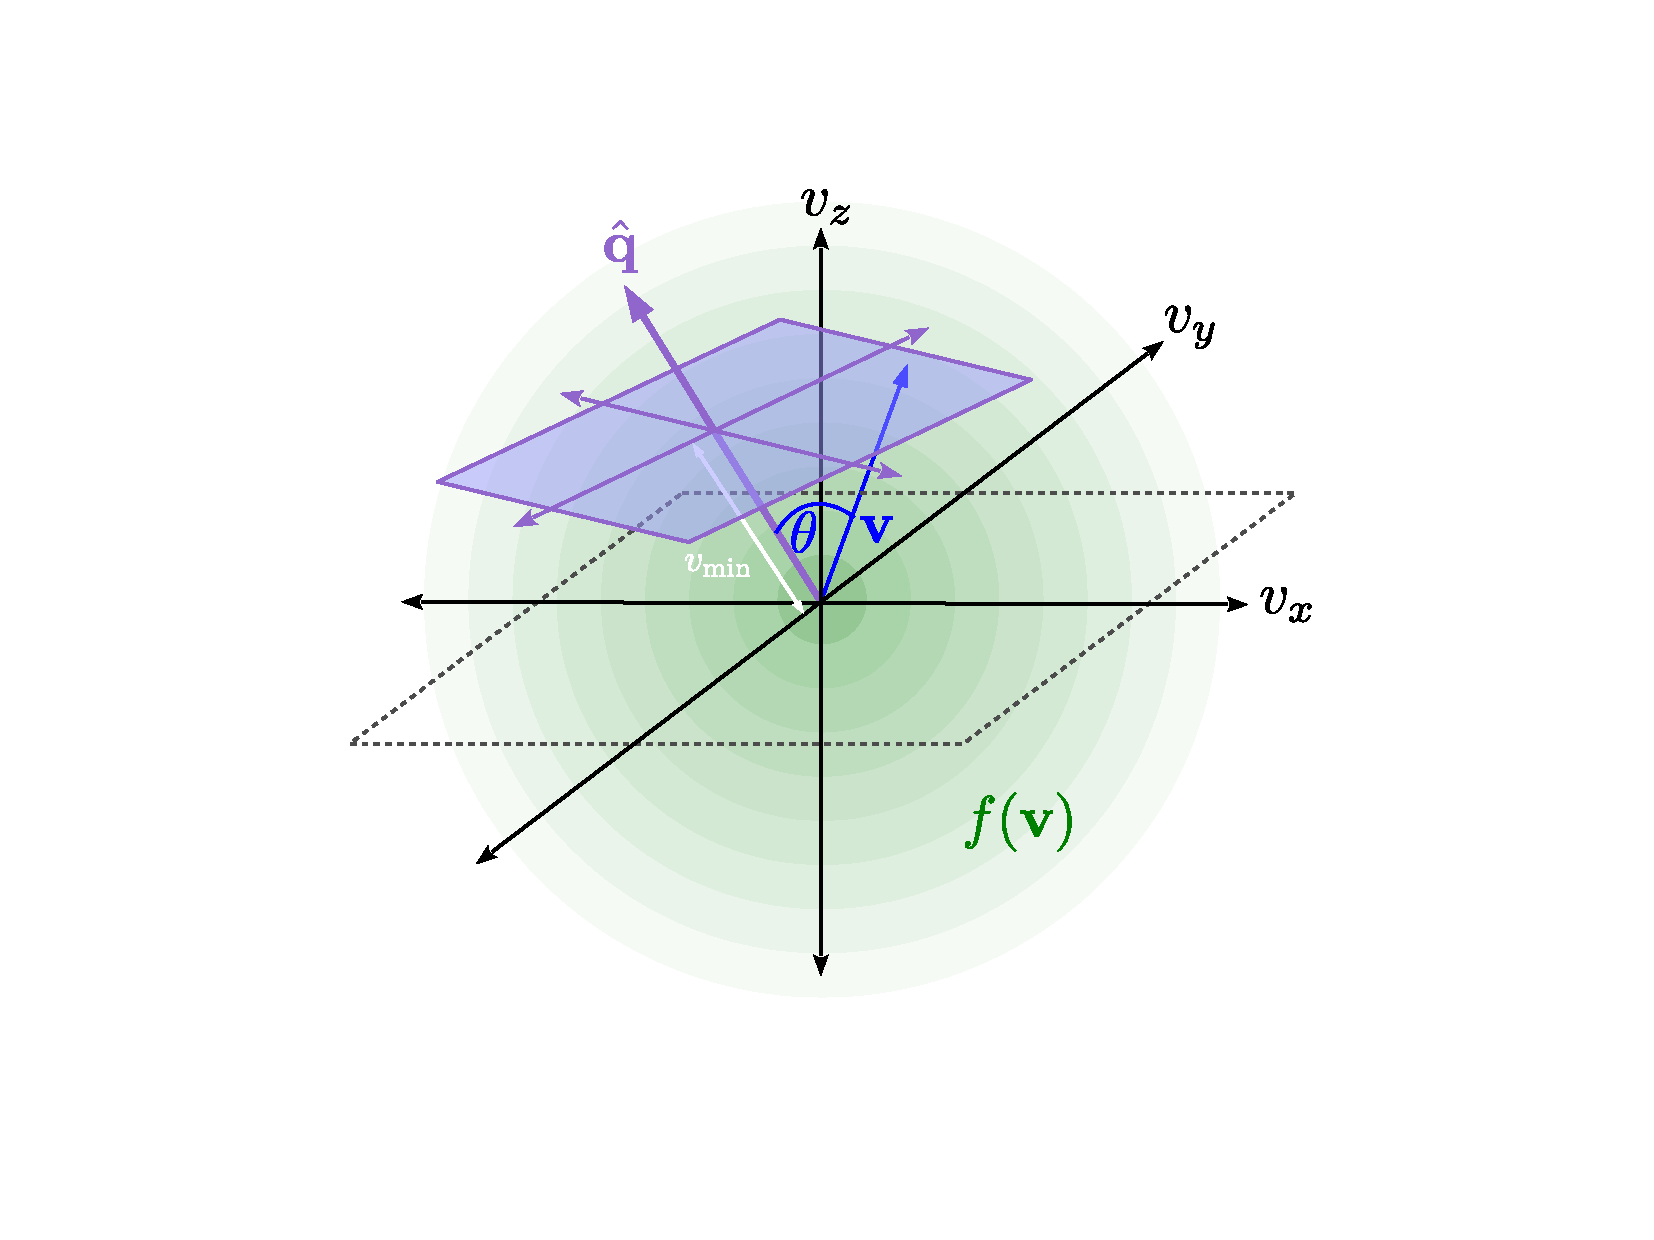
\includegraphics[trim = 20mm 30mm 20mm 20mm, clip, width=\textwidth]{Figures/radontransform.pdf}
	\caption[Diagram showing the geometry of the Radon transform]{Diagram showing the geometric interpretation of the Radon transform. The velocities $\color{blue}{\textbf{v}}$ of the distribution $\color[rgb]{0,0.5,0}{f(\textbf{v})}$ that contribute to the event rate for a particular $v_\textrm{min}$ and recoil direction $\color[rgb]{0.5686    0.4000    0.8000}{\hat{\textbf{q}}}$ are those which lie along the plane shown in purple. The plane is perpendicular to $\color[rgb]{0.5686    0.4000    0.8000}{\hat{\textbf{q}}}$ and is a distance $\vmin$ away from the origin. Thus the radon transform $\hat{f}(\vmin,\hat{\textbf{q}})$ is the integral of $\color{blue}{\textbf{v}}$ over the plane.}
	\label{fig:radontransform}
\end{figure}

In analogy with Eq.~(\ref{eq:finaleventrate}) we can write the general formula for the directional event rate,
\begin{equation}\label{eq:finaleventrate-directional}
 \frac{\textrm{d}^2R(t)}{\textrm{d}E_r\textrm{d}\Omega_r} = \sum_{i=1}^n \zeta^i \frac{\rho_0}{4\pi\mu_{\chi p}^2 m_\chi} (\sigma^{\rm SI}_p \mathcal{C}^i_{\textrm{SI}} F^2_{\rm SI}(E_r) + \sigma^{\rm SD}_p \mathcal{C}^i_{\textrm{SD}} F^2_{\rm SD}(E_r))  \, \hat{f}(\vmin,\hat{\textbf{q}},t) \, .
\end{equation}
This formula is very similar to the non-directional rate except we have picked up a factor of $1/2\pi$ and require $\hat{f}(\vmin,\hat{\textbf{q}},t)$ instead of $g(\vmin,t)$.

For the Maxwell-Boltzmann distribution of the SHM the Radon transform is,
\begin{equation}
\hat{f}_{\rm SHM}(v_{\text{min}},\hat{\bf{q}}, t) =
\begin{cases}
\frac{\exp{\left(-\frac{\left|v_{\text{min}} + \hat{\bf{q}}\cdot{\bf v}_{\rm lab}(t)\right|^2}{2\sigma^2_v}\right)} - \exp{\left(-\frac{v_{\rm esc}^2}{2\sigma^2_v}\right)}}{N_{\rm esc}(2\pi\sigma_v^{2})^{1/2}} & (\vmin + \hat{\textbf{q}} \cdot  \textbf{v}_\textrm{lab}(t))< \vesc \\
0 & (\vmin + \hat{\textbf{q}} \cdot  \textbf{v}_\textrm{lab}(t))> \vesc \, .
\end{cases}
\end{equation} 
While for the stream we have the same functional form but we replace $\sigma_v$ with $\sigma_{\rm str}$ and $\textbf{v}_\textrm{lab}$ with $\textbf{v}_\textrm{lab}+\textbf{v}_\textrm{str}$. 

For the debris flow we have the following form for the Radon transform,
\begin{equation}
\hat{f}_{\rm DF}(v_{\text{min}},\hat{\bf{q}}, t)  = 
\begin{cases}
0 & (\vmin + \hat{\textbf{q}} \cdot  \textbf{v}_\textrm{lab}(t))> v_f \\
\frac{1}{2v_f} & (\vmin + \hat{\textbf{q}} \cdot  \textbf{v}_\textrm{lab}(t))< v_f 
\end{cases}
\end{equation}
Because the distribution of a debris flow is a shell of radius $v_f$ centered on $\textbf{v}_\textrm{lab}$, its Radon transform is the integral along the circle that is the intersection of this shell and the plane shown in Fig.~\ref{fig:radontransform}.


\subsection{Resulting signals}\label{sec:directional_signals}
\begin{figure}
	\centering
	%trim option's parameter order: left bottom right top
	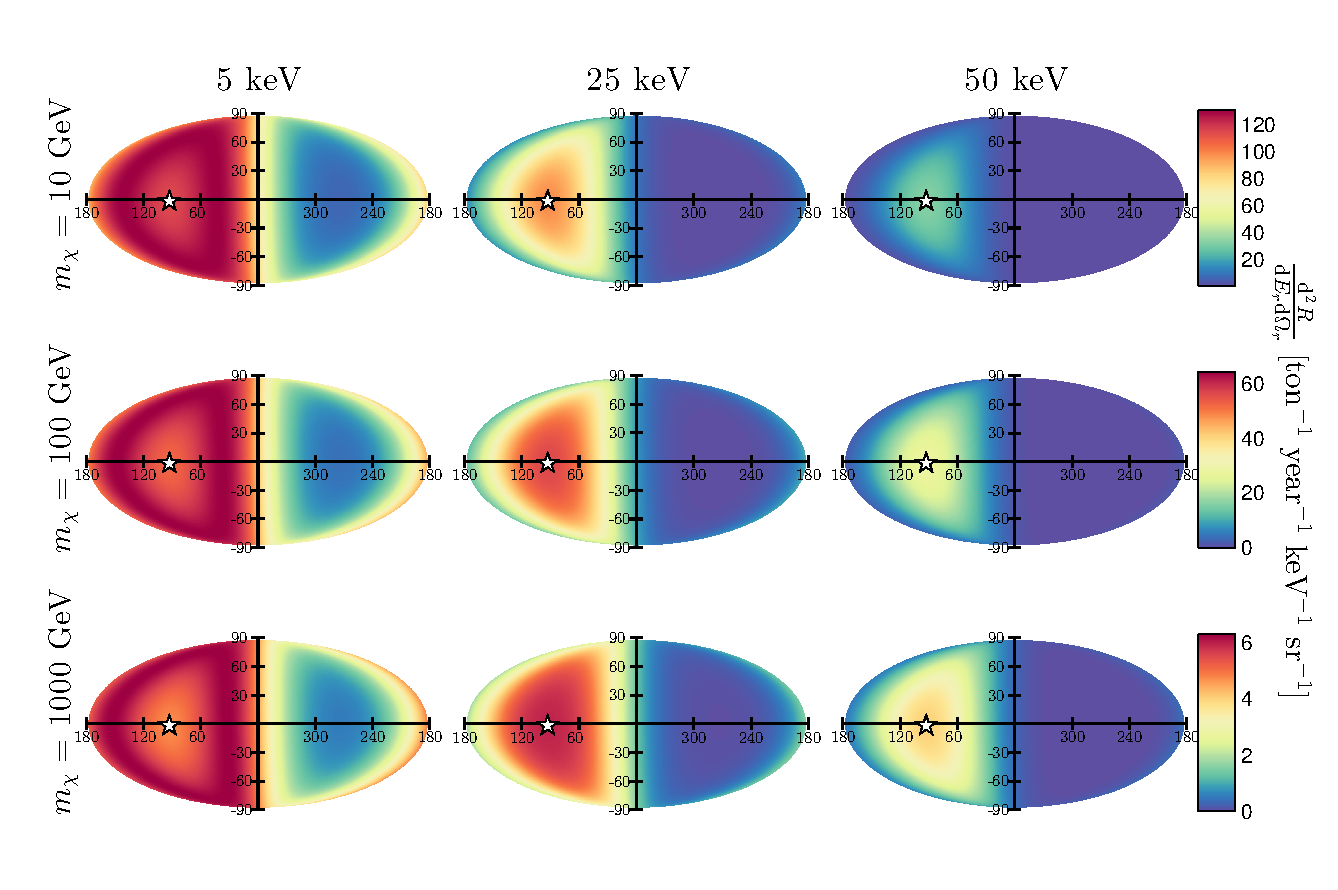
\includegraphics[trim = 0mm 0mm 0mm 0mm, clip, width=\textwidth]{Figures/skymaps_mchi.eps}
	\caption[Directional recoil skymaps for three WIMP masses]{Mollweide projections of the full sky recoil maps for three recoil energies: 5 keV, 25 keV and 50 keV corresponding to the three columns. The rows indicate recoil spectra for three WIMP masses $m_\chi = $ 10, 100 and 1000~GeV scattering with a $^{19}$F target. The axes represent Galactic coordinates $(l,b)$ where the direction of $\textbf{v}_\textrm{lab}$ is marked with a star.}
	\label{fig:skymaps_mchi}
\end{figure}

The event rate of Eq.~(\ref{eq:finaleventrate-directional}) gives rise to a range of unique directional signatures. The primary signal is a dipole anisotropy towards the direction $\hat{\bf{q}} = -{\bf v}_{\rm lab}$ as can be seen in Fig.~\ref{fig:skymaps_mchi} where we show the event rate as a function of energy and direction which clearly peaks along the plane of the Galaxy. As first calculated in Ref.~\cite{Spergel:1987kx} this would result in an $\mathcal{O}(10)$ forward-backward asymmetry in the number of recoils. In Fig.~\ref{fig:skymaps_mchi} and subsequent skymaps we use a Mollweide projection to map the 3-dimensional recoil spectrum onto the 2-d plane. We follow the convention used in directional detection literature to display recoil maps as the directions from which the recoils originate (as one would in astronomy) rather than the direction the recoils vectors point. In other words, the axes of the projection correspond to $-\hat{\textbf{q}}$ rather than $\hat{\textbf{q}}$. This is why the skymaps peak around the point marked by $\textbf{v}_\textrm{lab}$. This direction lies along the Galactic plane ($b_{\rm lab}~\approx~0$) and towards the direction of Galactic rotation ($l_{\rm lab}~\approx~90^\circ$), but is slightly offset by the Solar peculiar velocity $\textbf{v}_\odot$.

Because we assume an isotropic assumption for the Galactic frame velocity distribution the recoil maps are symmetric about the direction $\textbf{v}_\textrm{lab}$. The recoil directions also become less angularly dispersed towards higher recoil energies which preserve more of the original incoming WIMP direction. The prominence of the dipole feature means that in ideal circumstances (i.e. perfect recoil direction reconstruction) an isotropic assumption for the recoil direction distribution can be rejected at 90\% confidence with only $\mathcal{O}(10)$ events, with no recoil energy information needed~\cite{Green:2010zm}. With $\mathcal{O}(30)$ recoil directions it becomes possible to point back towards Cygnus and confirm the Galactic origin of the signal~\cite{Billard:2009mf}.

It was noted in Ref.~\cite{Bozorgnia:2011vc} that for recoil energies where $v_{\rm min}<v_{\rm lab}$ the directional rate is maximised for directions that satisfy $\hat{\bf{q}}\cdot{\bf v}_{\rm lab} = -v_{\rm min}$. At these energies the recoil pattern forms a ring around $\textbf{v}_{\rm lab}$, rather than a dipole. This occurs only for low energies and large WIMP masses but can be used as a secondary signal in directional detection as its radius would provide a measure of $m_\chi$. The ring feature has an angular radius of $\cos^{-1}(\vmin/v_\textrm{lab})$ and can be seen in Fig.~\ref{fig:skymaps_mchi} in the maps at $E_r = 5$~keV, most prominently in the $m_\chi=1000$~GeV case. Additionally, once the correlation with the time dependence is included then an aberration of the recoil pattern is observed (in analogy with the aberration of the position of stars in the sky due to the Earth's orbit~\cite{Bozorgnia:2012eg}). In our analyses we do not consider the ring or aberration features separately, as in Refs.~\cite{Bozorgnia:2011vc, Bozorgnia:2012eg} for example, but because they are embedded in the analytic description of the event rate they are included in likelihood fits automatically.

\subsection{Experiments}\label{sec:directional_expts}
The strength of directional detection as a tool for dark matter discovery relies on the fact that no known backgrounds are believed to mimic (or even have any relation to) the directionality of the dark matter signal. In fact most backgrounds should be close to isotropic. Certainly in the case of radiogenic neutrons an essentially isotropic background is expected. Cosmic muon induced neutrons would not necessarily be expected to be perfectly isotropic, however past studies~\cite{Mei:2005gm} have found only a very small downward-going excess due to the directionality of spallation reactions. The elastic scattering process also washes out much of the directional preference in the flux of incoming particles so any backgrounds would need to be very strongly anisotropic to affect the discovery reach of a directional experiment.

\begin{figure}
	%trim option's parameter order: left bottom right top
	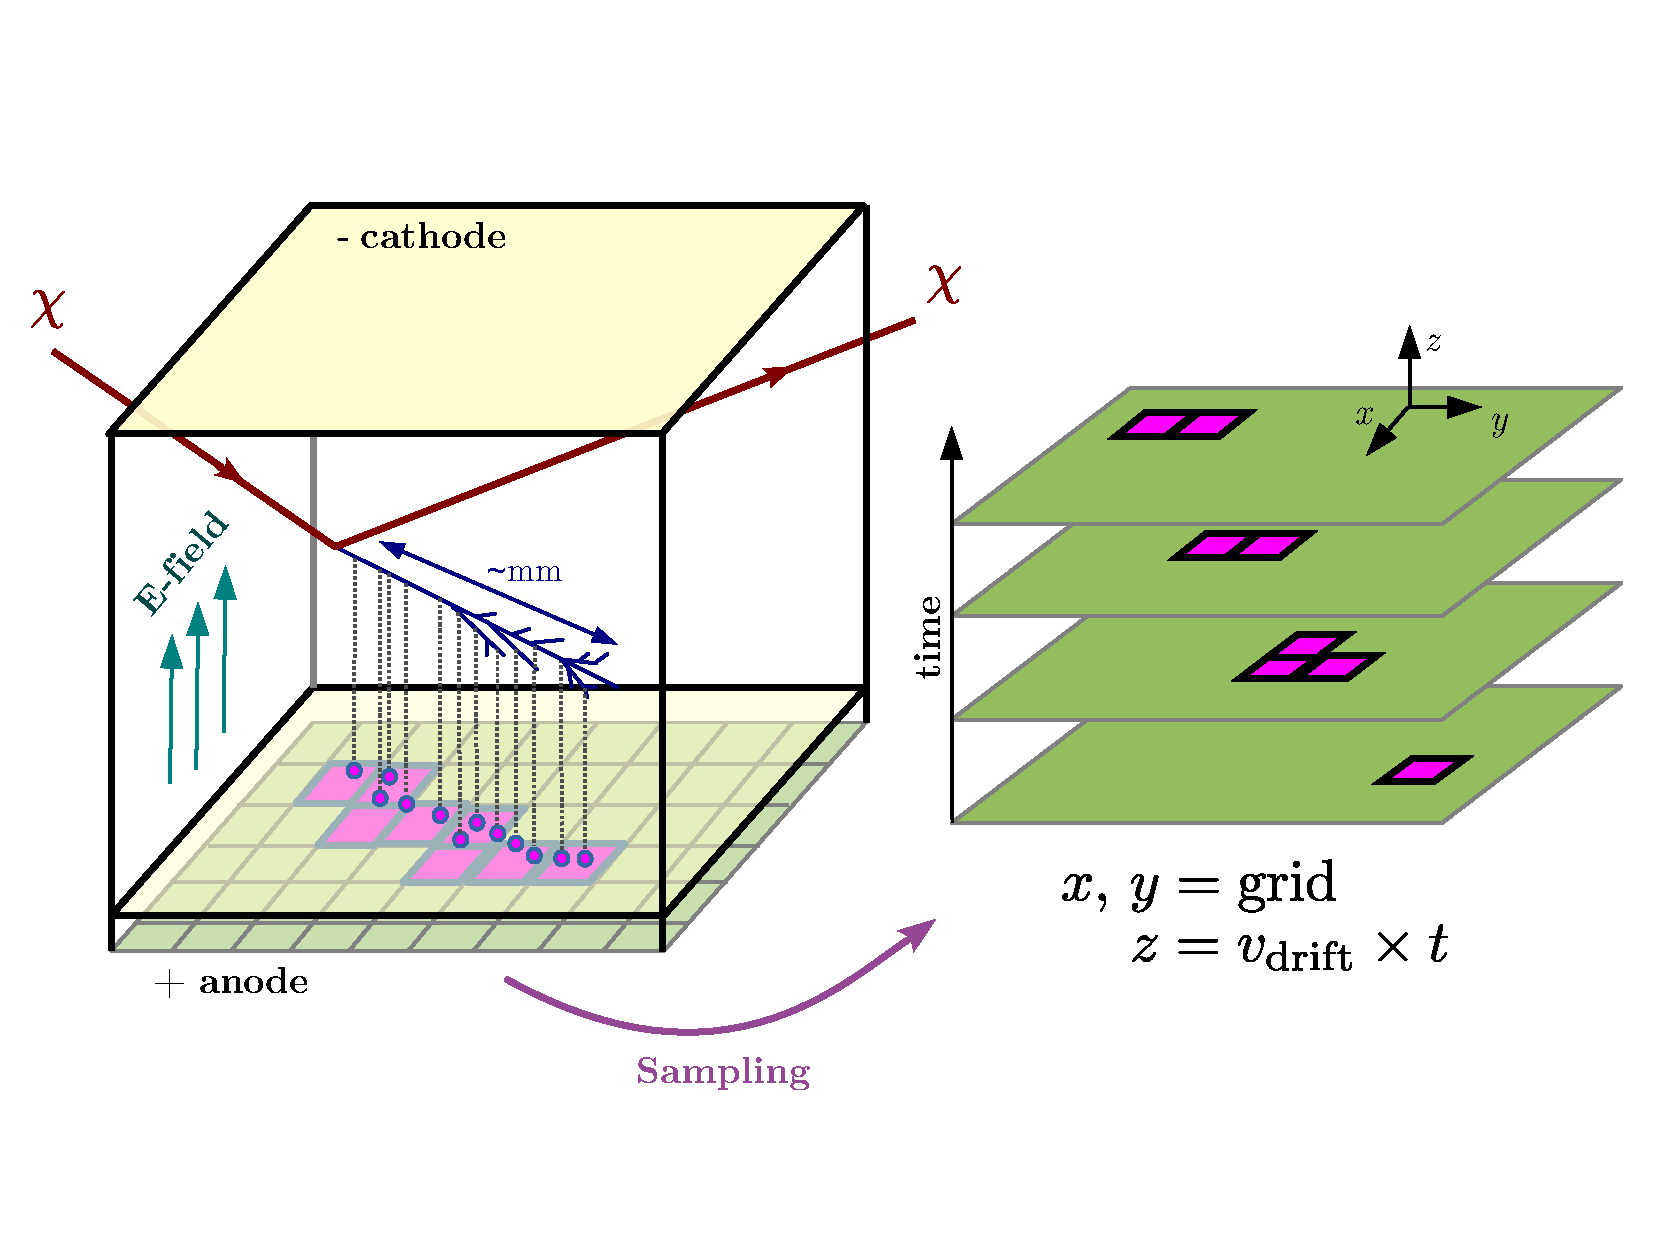
\includegraphics[trim = 0mm 20mm 0mm 20mm, clip, width=\textwidth]{Figures/TPC.pdf}
	\caption[Diagram of a low pressure gas TPC]{Diagram of a low pressure gas TPC with a pixel chip readout.}
	\label{fig:TPC}
\end{figure}

Measuring the direction of nuclear recoils at the keV scale is experimentally challenging. A variety of prototype experiments are currently in operation utilising a range of novel techniques to extract directional information from a nuclear recoil signal (see e.g.~Refs.~\cite{Cappella:2013,Capparelli:2014lua,Aleksandrov:2016fyr}, as well as Ref.~\cite{Ahlen:2009ev} for a review). One promising approach is to use a gaseous TPC at low pressure ($\sim$ 0.1 atm) in order for the track of electrons ionised by a nuclear recoil to be large enough to detect at around $\mathcal{O}(1\,{\rm mm})$ in size. In Fig.~\ref{fig:TPC} we show a diagram of how a low pressure TPC measures the components of a recoil track in three dimensions. The direction of this recoil can be inferred by drifting the ionisation-induced electron cloud to a time sampled pixelised anode usually based on CCD technology. The location on the grid of the measured charge provides a two dimensional projection of the track whereas the time sampling of the anode can be converted into the projection onto the drift direction assuming knowledge of the drift speed of the electrons through the gas, $v_{\rm drift}$. In principle these two effects can be combined to reconstruct the 3-dimensional orientation of the track. Experiments such as MIMAC~\cite{Riffard:2013psa,Riffard:2016mgw}, DRIFT~\cite{Daw:2011wq,Battat:2014van}, NEWAGE~\cite{Nakamura:2015iza,Miuchi:2010hn}, DMTPC~\cite{Monroe:2011er,Leyton:2016nit} and D3~\cite{Jaegle:2011rn} currently make use of this technology in some variant. 

Attempts to measure recoil directionality encounter a range of experimental difficulties on top of the usual challenges of direct detection. The most obvious limitation of low pressure TPCs operating in the gas phase is their ability to be scaled to competitive detector masses which would require prohibitively large volumes. The largest of these prototype experiments currently has only a 0.1 kg active volume~\cite{Santos:2011kf}, though a much larger WIMP `observatory' is a possibility~\cite{Simpson:2017aaa}. In terms of the operation of a directional TPC however, the greatest challenges are those that arise in attempting to accurately reconstruct the recoil track. Primarily this is because the detected track is not a perfect representation of the initial recoil direction $\hat{\textbf{q}}$. In practice experiments suffer from an effect known as `straggling' as the recoiling nucleus collides with other gas nuclei. When combined with the diffusion of the electron cloud while drifting toward the anode, this effect leads to a sizable angular resolution, limiting the accuracy with which a track direction can be reconstructed~\cite{Billard:2011kv}. In current gas TPC prototypes the best achievable angular resolution is around the tens of degrees level~\cite{Billard:2012bk}. In addition to obtaining good angular resolution, a head-tail effect - the measurement of the sense of the nuclear recoil ($+\qhat$ or $-\qhat$) - has proven to be difficult to achieve~\cite{Billard:2012bk,Majewski:2009an, Dujmic:2008zz}. Sense recognition is possible if there is some observable asymmetry along the track either in its geometry or the charge deposition that implies a beginning and end~\cite{Billard:2011kv}. When the angular recoil rates in the forward and background directions are summed, the anisotropy of the WIMP recoils is effectively decreased. Hence the lack of sense recognition has been shown to have a significant impact on the discovery potential of directional experiments~\cite{Green:2007at,Billard:2014ewa,Morgan:2004ys,Billard:2011zj,Copi:2005ya}. For this reason it is arguably the most important technical limiting factor for gas TPCs so we study the consequences of removing sense recognition in detail in Sec.~\ref{sec:folded} of this Chapter and Sec.~\ref{sec:nufloor_sense} of Chapter~\ref{chapter:nufloor}.

In some configurations the three dimensional readout of the track is not possible. Experiments like the pioneering detector of Buckland~\etal~\cite{Buckland:1994gc, Lehner:1997fs} that image recoils lengths by detecting photons produced along the track only have access to the 2-dimensional $x-y$ projection of the recoil direction. Moreover, though no experiment currently exists, one can also imagine a 1-dimensional version of a directional detector that would somehow involve just the projection onto the drift direction via timing resolution. Lower dimensional readout is another experimental restriction that would reduce the discovery reach of a directional experiment~\cite{Billard:2014ewa}. For a comprehensive review of experimental readout technologies see Ref.~\cite{Battat:2016pap}. We explore lower dimensional readout strategies in more detail when we discuss the neutrino floor in Chapter~\ref{chapter:nufloor}.

While low pressure gas TPCs are the most mature technologically, it may be possible to directionally detect dark matter with other techniques. Detectors using graphene~\cite{Hochberg:2016ntt,Wang:2015kya}, carbon nanotubes~\cite{Capparelli:2014lua}, or DNA~\cite{Drukier:2012hj} have been suggested as potential targets, though the feasibility of such methods is yet to be established. The NEWS collaboration is in R\&D towards an experiment using silver-halide emulsion plates~\cite{Aleksandrov:2016fyr} in which the sub-micrometer length recoil tracks are left as clusters of silver grains. The tracks would be detected and resolved by automated optical microscopes that scan the plates after the running of the experiment. Because the events are not time tagged it has been suggested that NEWS will be placed on an equatorial mount and pointed towards Cygnus, in order to remove the smearing of the angular recoil spectrum due to the rotation of the Earth.

Given the long standing efforts in scaling direct detection experiments to large masses, it may be more effective to try and extract some directional signals in existing experiments. A phenomenon known as `columnar recombination' may be such a signal and could be exploitable in existing dual phase liquid xenon or argon TPCs~\cite{Nygren:2013nda,Mohlabeng:2015efa,Li:2015zga,Cadeddu:2017ebu}. In principle the recombination between electrons and ions along recoils in liquid noble gases should be dependent on the angle between the track and the drift direction, so the subsequent ionisation signal may have some directional dependence. Columnar recombination would be an example of a 1-dimensional readout. This would also exhibit a characteristic modulation associated with the Earth's rotation which could change the ratio of horizontal to vertical events by a factor four over the course of a day~\cite{Cadeddu:2016mac}. Experimentally however this efficacy of columnar recombination has yet to be confirmed and ongoing measurements by the SCENE collaboration have only found mild evidence for it in keV-scale nuclear recoils~\cite{Cao:2014gns}. Lastly, we note that it may also be possible to exploit directionality in solid state detectors~\cite{Bernabei:2003ct}. Crystal scintillators made from ZnWO$_4$ have been shown to have highly anisotropic properties in their light output and pulse shape, compared to the standard NaI~\cite{Cappella:2013rua}. Such crystals have been suggested as a way to extend the technology of scintillators to a directional search.

\section{Detecting streams}\label{sec:directional_streams}
Given that direct detection experiments are the only way to probe the velocity distribution down to sub-milliparsec scales, a central goal of the post-discovery era will be to determine the quantity of substructure in the local DM halo. Because substructures can give rise to phenomenologically varied signatures in recoil spectra it will be useful to attempt to discriminate between different classes in a model-independent way. Our first study is of the particular case of substructure in the form of tidal streams. If present in the local velocity distribution as suggested by a number of observations and simulations~\cite{Newberg:2003cu,Yanny:2003zu,Majewski:2003ux,Purcell:2012sh,Luque:2016nsz}, streams would in many cases be difficult to notice in the non-directional recoil energy spectrum (unless they comprised a much larger fraction of the local density than expected). However, since tidal streams are highly kinematically localised structures they show up prominently in the directional spectrum. The possibility of detecting streams is therefore a very good motivation and physics case for directional detectors in general. The study we describe now attempts to explore how these detection prospects depend on the properties of the stream itself and involves a comparison of several statistical procedures for extracting the stream from simulated directional data.

The strategy we will follow involves two parts. We first establish the detectability of a stream by attempting to reject the hypothesis of a smooth isotropic halo model in favour of one in which some level of anisotropy is present suggesting the existence of a stream. After this step has been performed one may attempt to fit the anisotropy to a model for the stream and measure its parameters. To begin we consider non-parametric statistical tests. These tests use the direction information only and have been implemented in some previous studies which sought to establish the discovery potential of a DM signal over isotropic backgrounds~\cite{Morgan:2004ys, Green:2010zm}. The advantage of a non-parametric analysis in assuming no model to describe the data is that the results will be independent of the description of the background halo, as long as the basic hypotheses that define the statistical tests are satisfied. However a notable disadvantage is that the detection significance will always be lower if a model is not chosen, hence we will subsequently perform a parametric likelihood analysis and fit the data to a model for the stream.

\subsection{Stream model}\label{sec:directional_streammodels}
As introduced in the previous Chapter a stream can be modelled with Maxwellian velocity distribution offset by the stream velocity $\textbf{v}_\textrm{str}$ and a reduced velocity dispersion $\sigma_{\rm str}\sim 10$~km~s$^{-1}$. The SHM+Str model consists of splitting the full velocity distribution into a smooth halo component described by the usual Maxwellian, and a stream which comprises a fraction $\xi_{\rm str} = \rho_{\rm str}/\rho_0$ of the local density. The Radon transform is linear in $f(\textbf{v})$ so the directional event rate for the SHM+Str model simply sums the contributions from the SHM and the stream with the appropriate weighting of $(1-\xi_{\rm str})$ and $\xi_{\rm str}$ respectively. Figure \ref{fig:streamskymap} shows the angular and energy dependence of the Radon transform (which reflects the angular dependence of the full event rate) for the SHM+Str distribution with parameters from Table~\ref{tab:astrobenchmarks}.
\begin{figure}
	\centering
	%trim option's parameter order: left bottom right top
	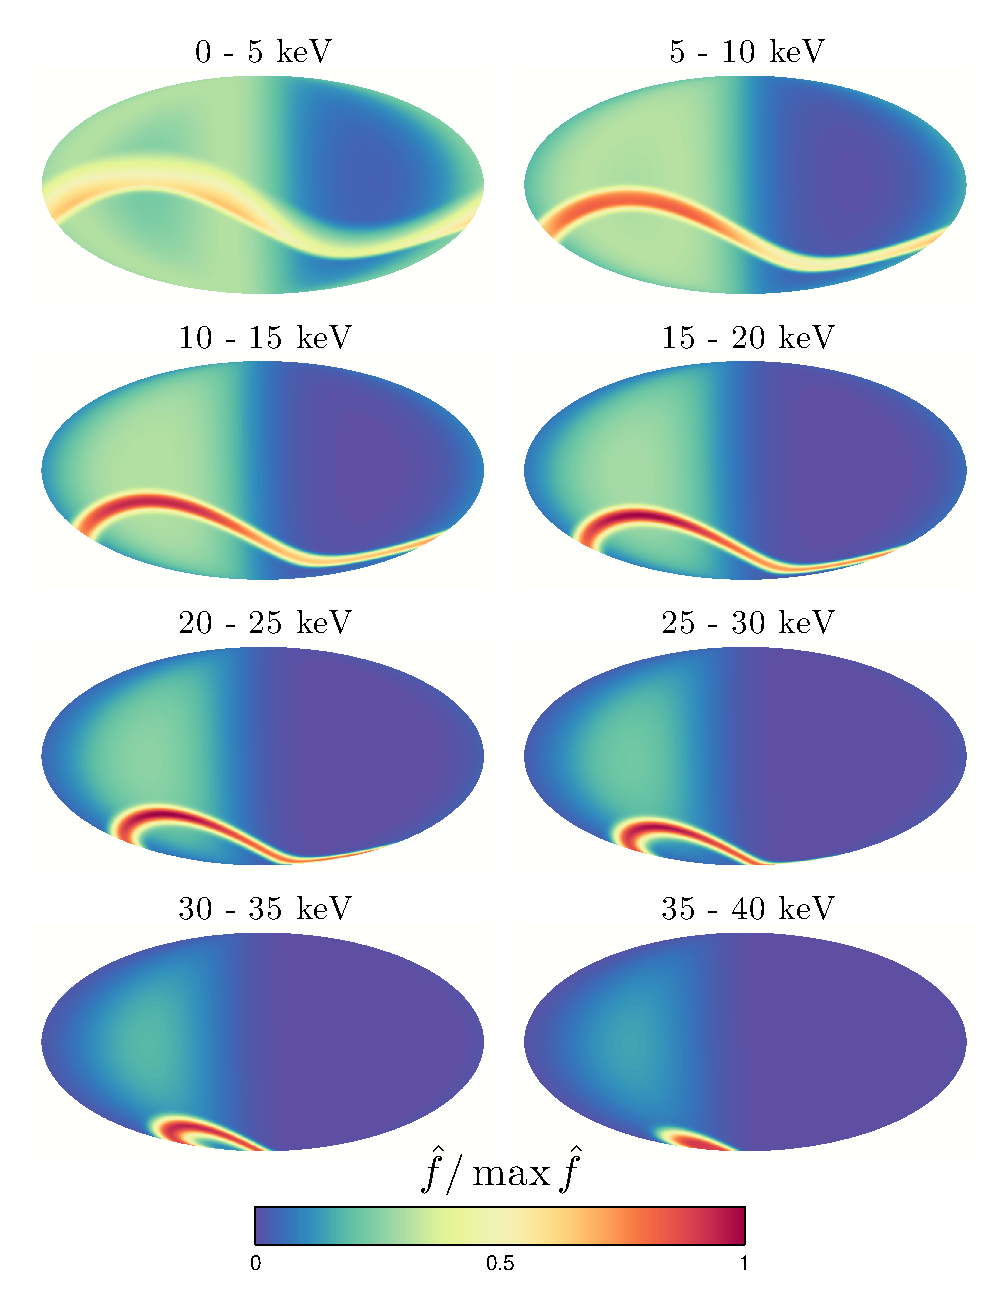
\includegraphics[trim = 0mm 0 0mm 0mm, clip, width=0.8\textwidth]{Figures/streamskymap.eps}
	\caption[Directional recoil skymaps for the SHM+Stream model]{Mollweide projection skymaps of the rescaled Radon transform integrated over 5 keV bins in energy. The recoil pattern corresponds to the SHM+Str velocity distribution where we use the example of the Sagittarius stream and a $m_\chi = 50$ GeV WIMP scattering off $^{19}$F.}
	\label{fig:streamskymap}
\end{figure}

The parameters used to describe the stream are $\xi_{\rm str}$, $\textbf{v}_\textrm{str}$ and $\sigma_\textrm{str}$. When describing the properties of the stream we will also often express its direction in terms of the angle between $\textbf{v}_\textrm{str}$ and $\textbf{v}_\textrm{lab}$,
\begin{equation}\label{eq:deltatheta}
      \Delta \theta = \cos^{-1}\left(\frac{\textbf{v}_\textrm{lab} \cdot \textbf{v}_\textrm{str}}{v_{\rm str} v_{\rm lab}}\right).
\end{equation}
Because of the azimuthal symmetry in the SHM+Str model about $\textbf{v}_{\rm lab}$, the number of events originating from the stream will only depend on the stream direction through this parameter. This angle we define using the Galactic frame descriptions of $\textbf{v}_\textrm{str}$ and $\textbf{v}_\textrm{lab}$.

Formally the question we wish to answer is; how many events are needed to reject at a given confidence level a smooth and isotropic halo in the case that the true distribution possesses an additional substructure component? In Fig.~\ref{fig:signal_comparison_skymap} the problem is displayed visually; how does one extract information about a stream from some set of spherical data collected over a short exposure? The left hand panels show the normalised directional signal observed in a perfect detector with infinite exposure, under the astrophysical parameters given in Table \ref{tab:partable}. The top two panels displaying the signal with no stream present, and the bottom after inclusion of the stream. The right hand panels show an example of the signal expected in a detector over an exposure of $\mathcal{E}=10$ kg yr, including the signal from isotropic experimental backgrounds. The data have been binned on a sphere using a HEALPix \cite{Gorski:2004by} equal angular area discretisation with 768 pixels. Statistical tests must be able to distinguish between these two types of signal. Whilst detecting the directionality of the signal thus confirming the Galactic origin of the scattering particle requires few events, confirming deviations from a smooth halo will require a larger number.

In most of the following results unless otherwise stated we fix to a single WIMP particle benchmark\footnote{At the time when this study was originally conducted this benchmark was not excluded by constraints from direct detection experiments but has since been excluded by PICO-60~\cite{Amole:2017dex}.}, namely a WIMP with a mass of $m_\chi = 50 \, \, \mathrm{GeV}$ and a solely SD WIMP-nucleon cross section of $\sigma^{\rm SD}_p = 10^{-39} \, \, \mathrm{cm}^2$. This is primarily for clarity in describing our results. We do of course expect our results to be dependent on this choice however we do not expect that varying it will be particularly insightful for understanding the working of our statistical tests. Our mock experiment is based on a $^{19}$F target, inspired by existing low pressure gas TPCs with CF$_4$ such as NEWAGE~\cite{Nakamura:2015iza,Miuchi:2010hn} and DMTPC~\cite{Leyton:2016nit}. For simplicity we neglect in all the results in this Chapter the time dependence of $\textbf{v}_{\rm lab}$ which is mostly unimportant for the event numbers we consider here. In the following Chapter we extend to a full direction+energy+time analysis.

\begin{figure}
    \centering
    %trim option's parameter order: left bottom right top
    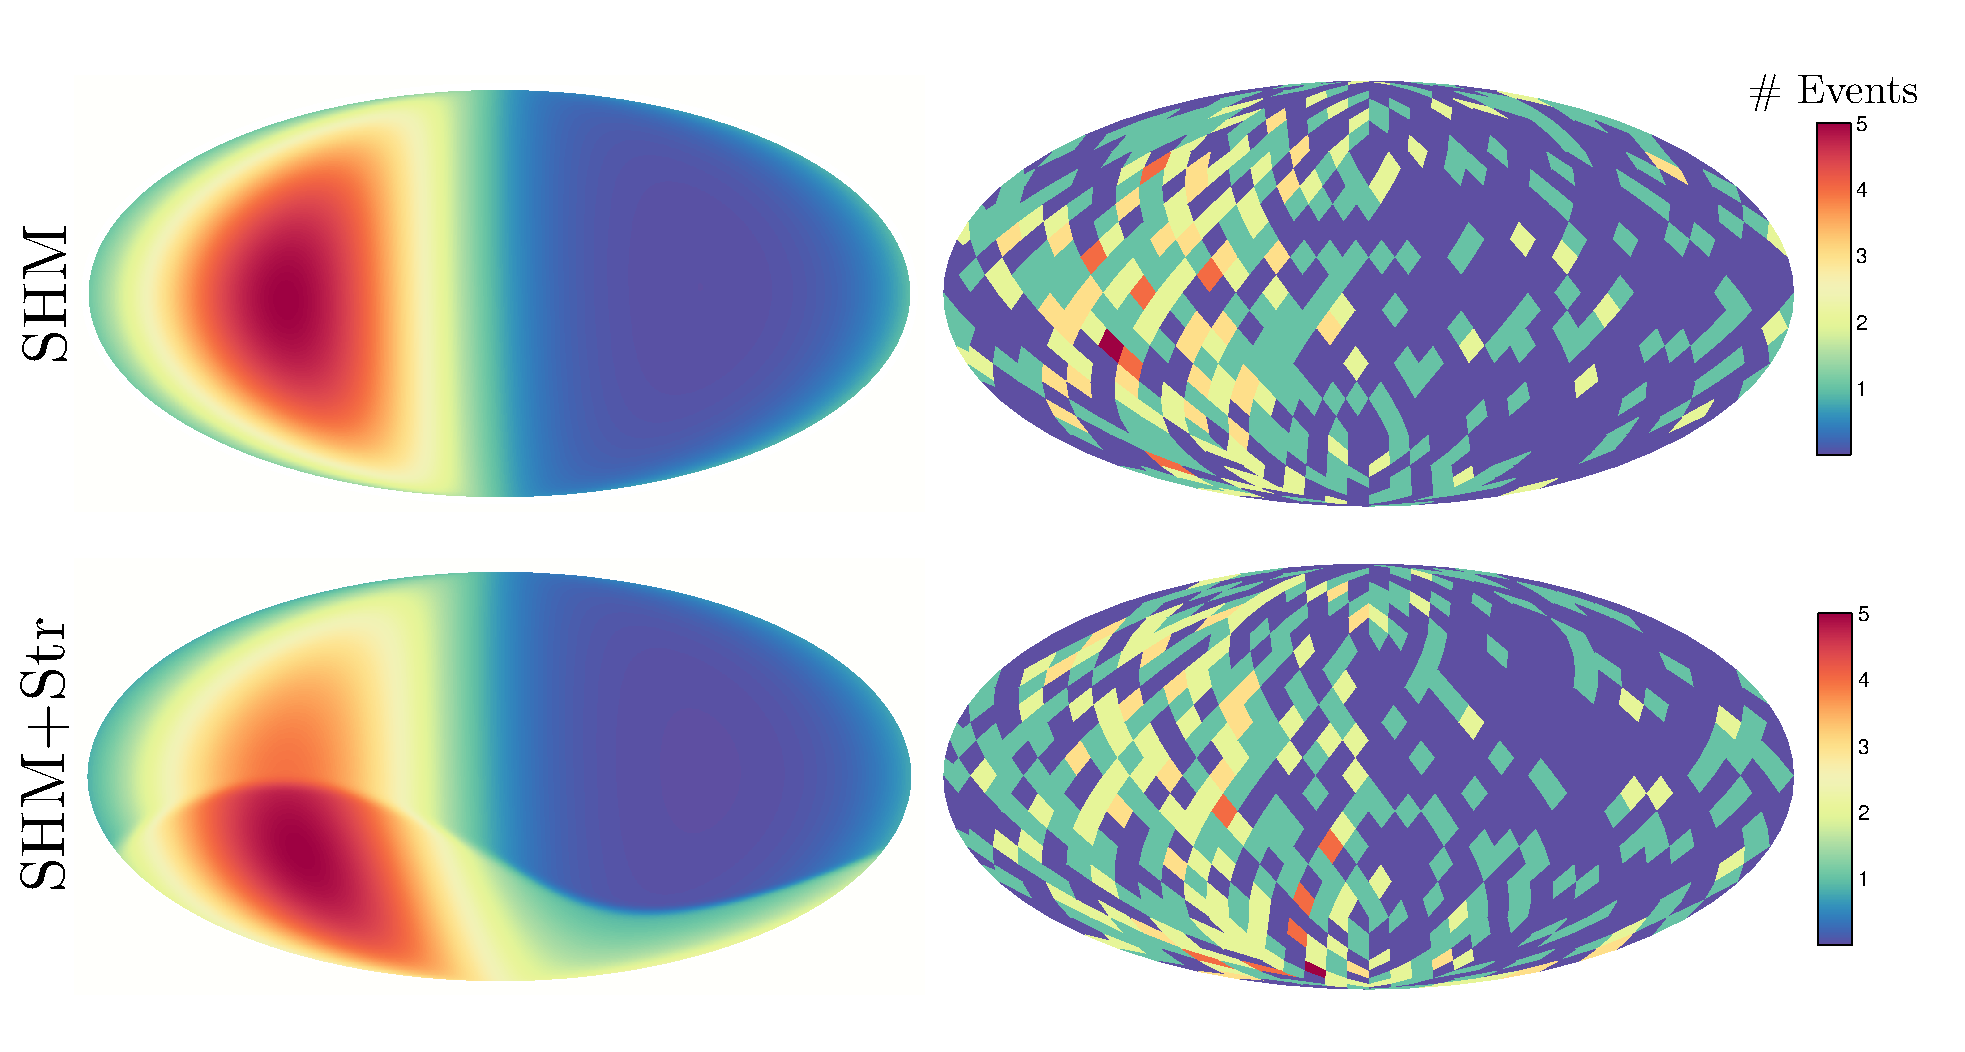
\includegraphics[trim = 0mm 0mm 0mm 0mm, clip, width=0.99\textwidth]{Figures/signal_comparison_skymap.eps}
    \caption[Simulated data for the SHM and SHM+Stream models]{SHM (top row) and SHM+Str (bottom row) direction-only signals for the underlying distribution (left column) and a set of data (right column) with an isotropic experimental background present. The signals are for a 50 GeV WIMP and astrophysical parameters from Table~\ref{tab:astrobenchmarks}. Our mock experiment uses a $^{19}$F target and in this case an energy sensitive window of $[5,100]$~keV. The datasets on the right are for a 10 kg yr exposure and a signal fraction of 0.5.}
    \label{fig:signal_comparison_skymap}
\end{figure}

\subsection{Non-parametric statistics}\label{sec:directional_nonparametric}
We can test for the presence of streams in the velocity distribution with statistics designed for spherical data. The general procedure involves first extracting some statistic $\mathcal{T}>0$ from the data that is distributed according to $p_0(\mathcal{T})$ under a null hypothesis (no stream present, $\xi_{\rm str}=0$) and $p_1(\mathcal{T})$ under an alternative hypothesis (stream present, $\xi_{\rm str}>0$). For some statistics these distributions may be known analytically but if not they can be built with a Monte Carlo simulation. For a particular result $\mathcal{T}_\textrm{obs}$ we define the `significance' to be the probability of measuring $\mathcal{T}<\mathcal{T}_\textrm{obs}$ if the null hypothesis is true,
\begin{equation}\label{eq:significance}
	S = \int_{0}^{\mathcal{T}_\textrm{obs}} p_0(\mathcal{T}) \textrm{d}\mathcal{T}.
\end{equation}   
We also define the statistical power as the probability of rejecting the null hypothesis if the alternative hypothesis is true. In other words it is the probability of measuring $\mathcal{T}>\mathcal{T}_\textrm{obs}$ in the alternative case,
\begin{equation}
	P = \int_{\mathcal{T}_\textrm{obs}}^{\infty} p_1(\mathcal{T})\textrm{d}\mathcal{T} \, .
\end{equation}
We build these two distributions from the repeated application of the statistical test on Monte Carlo generated Poisson datasets\footnote{For the details of the scattering simulation used to generate directional detection data see Appendix~\ref{app:scattering}.} for a particular set of input parameters. We then find the value of $\mathcal{T}$ for which $P=0.95$, i.e. the value achievable in 95\% of hypothetical experiments. Our results can then be expressed in units of $S_{95}$ calculated from $p_0$ at the same value of $\mathcal{T}$; $S_{95}$ is therefore the minimum detection significance achievable in 95\% of experiments.

There are two appropriate statistical procedures we can use to test for the existence of streams. The first test is a median direction test where the statistic follows a $\chi^2$ distribution for a set of data that has a median direction along some predicted direction. The second test is based on the modified Kuiper statistic, $V^\star$, and measures the degree to which a set of data has rotational symmetry about some predicted direction. In both cases we set the predicted direction satisfied by the null hypothesis to $\hat{\textbf{x}}_\textrm{lab}~=~-\textbf{v}_\textrm{lab}/v_{\rm lab}$. Details about the calculation of these test statistics can be found in Appendix~\ref{app:dirstats}.

\begin{figure}
      \centering
      %trim option's parameter order: left bottom right top
      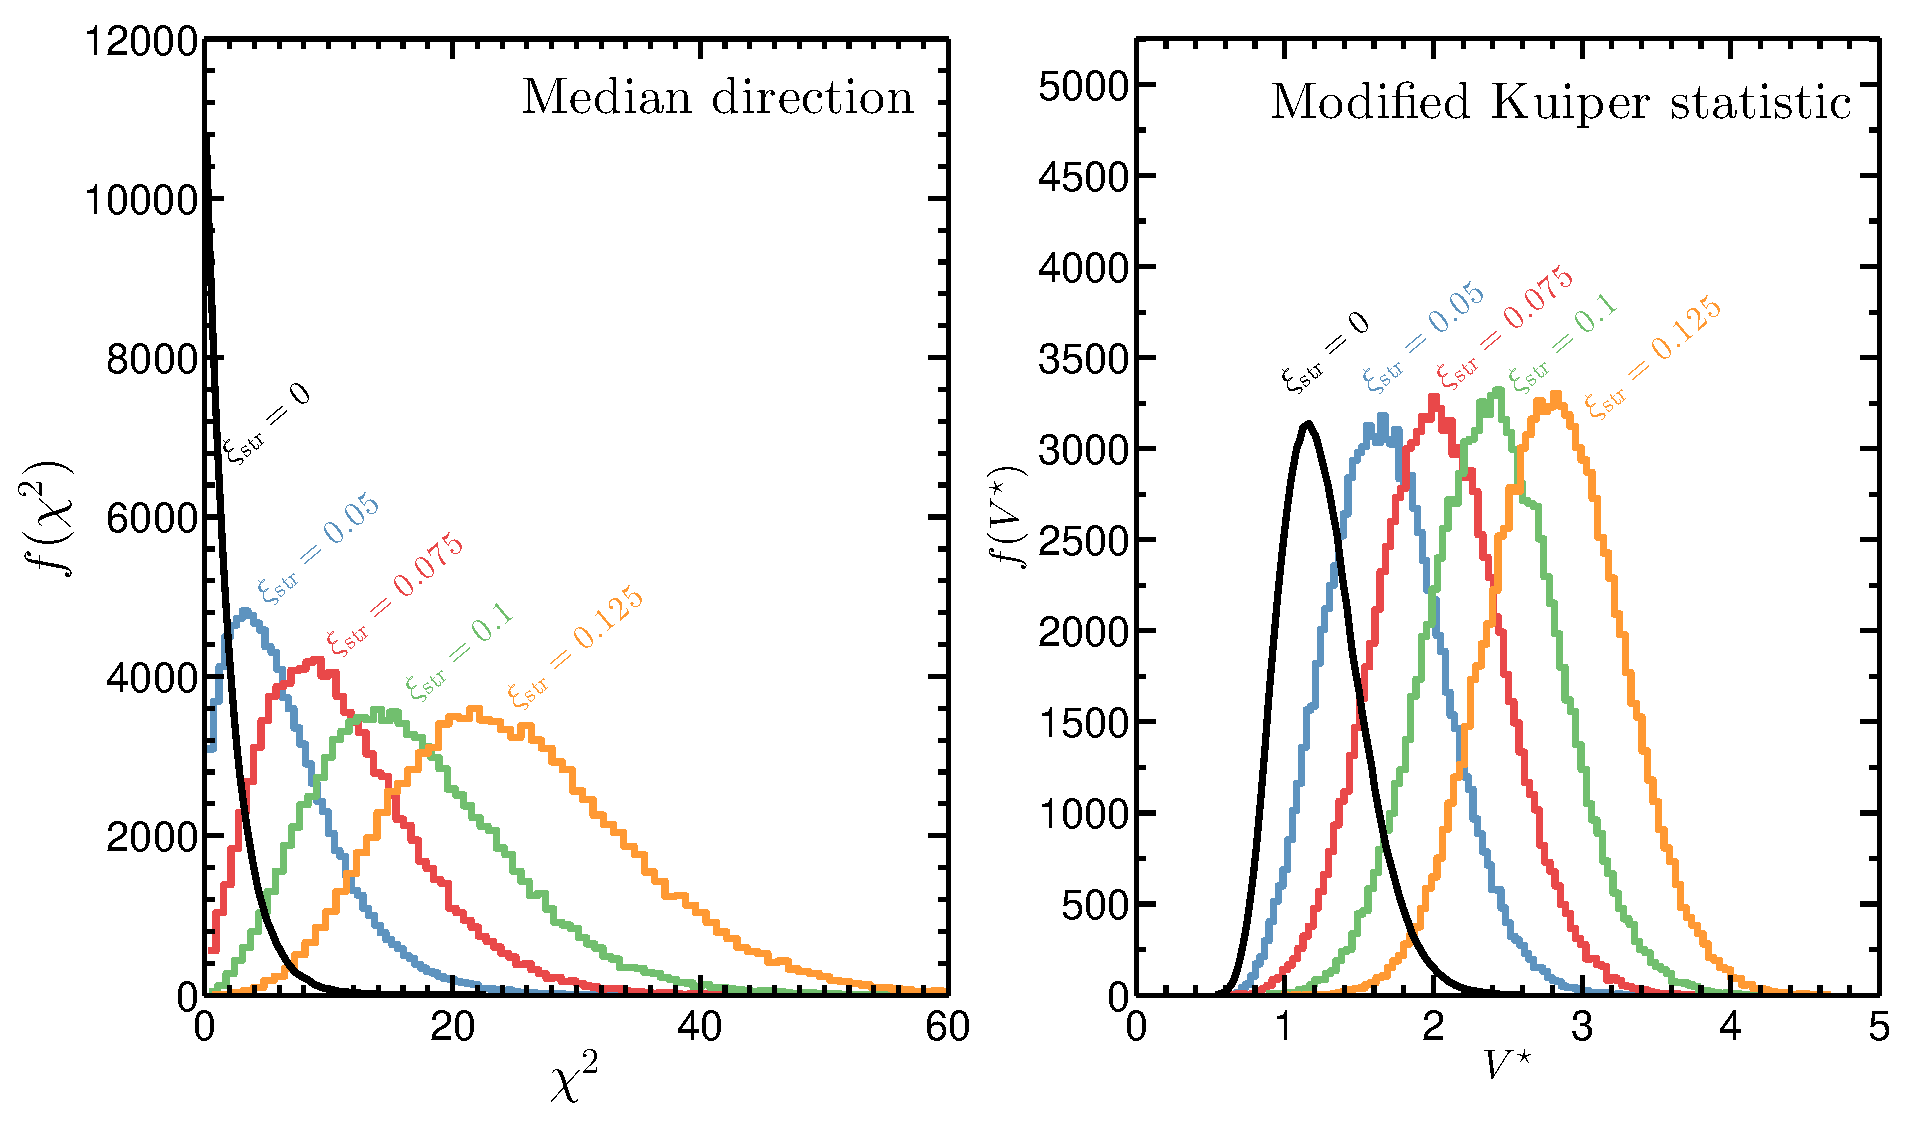
\includegraphics[trim = 0mm 0mm 0mm 0mm, clip, width=0.99\textwidth]{Figures/dirstatsdists.eps}
      \caption[Distributions of statistics for varying stream densities]{Distributions of the median direction $\chi^2$ statistic, and Kuiper statistic, $V^\star$,  built from $10^5$ Monte Carlo mock experiments. The distributions compare the case when there is no stream  present ($\xi_{\rm str} = 0$, black curve) and for streams of varying fractions ($\xi_{\rm str} > 0$, coloured histograms increasing left to right) cases.}
      \label{fig:dirstatsdists}
\end{figure}
Examples of the distributions of the statistics with a stream present as well as the distributions in the null case are shown in Fig.~\ref{fig:dirstatsdists}. The distributions in each case were generated from $10^5$ mock experiments with an exposure of $\mathcal{E} = 10$~kg~yr. As $\xi_{\rm str}$ is increased the signal becomes more influenced by the stream and hence the degree of rotational asymmetry is increased and the median direction becomes more displaced from $\hat{\textbf{x}}_\textrm{lab}$. We see this in the distributions of the statistics, for cases which disagree more with the null hypothesis, their distributions are further from the null distribution.

\begin{figure}
    \centering
    %trim option's parameter order: left bottom right top
    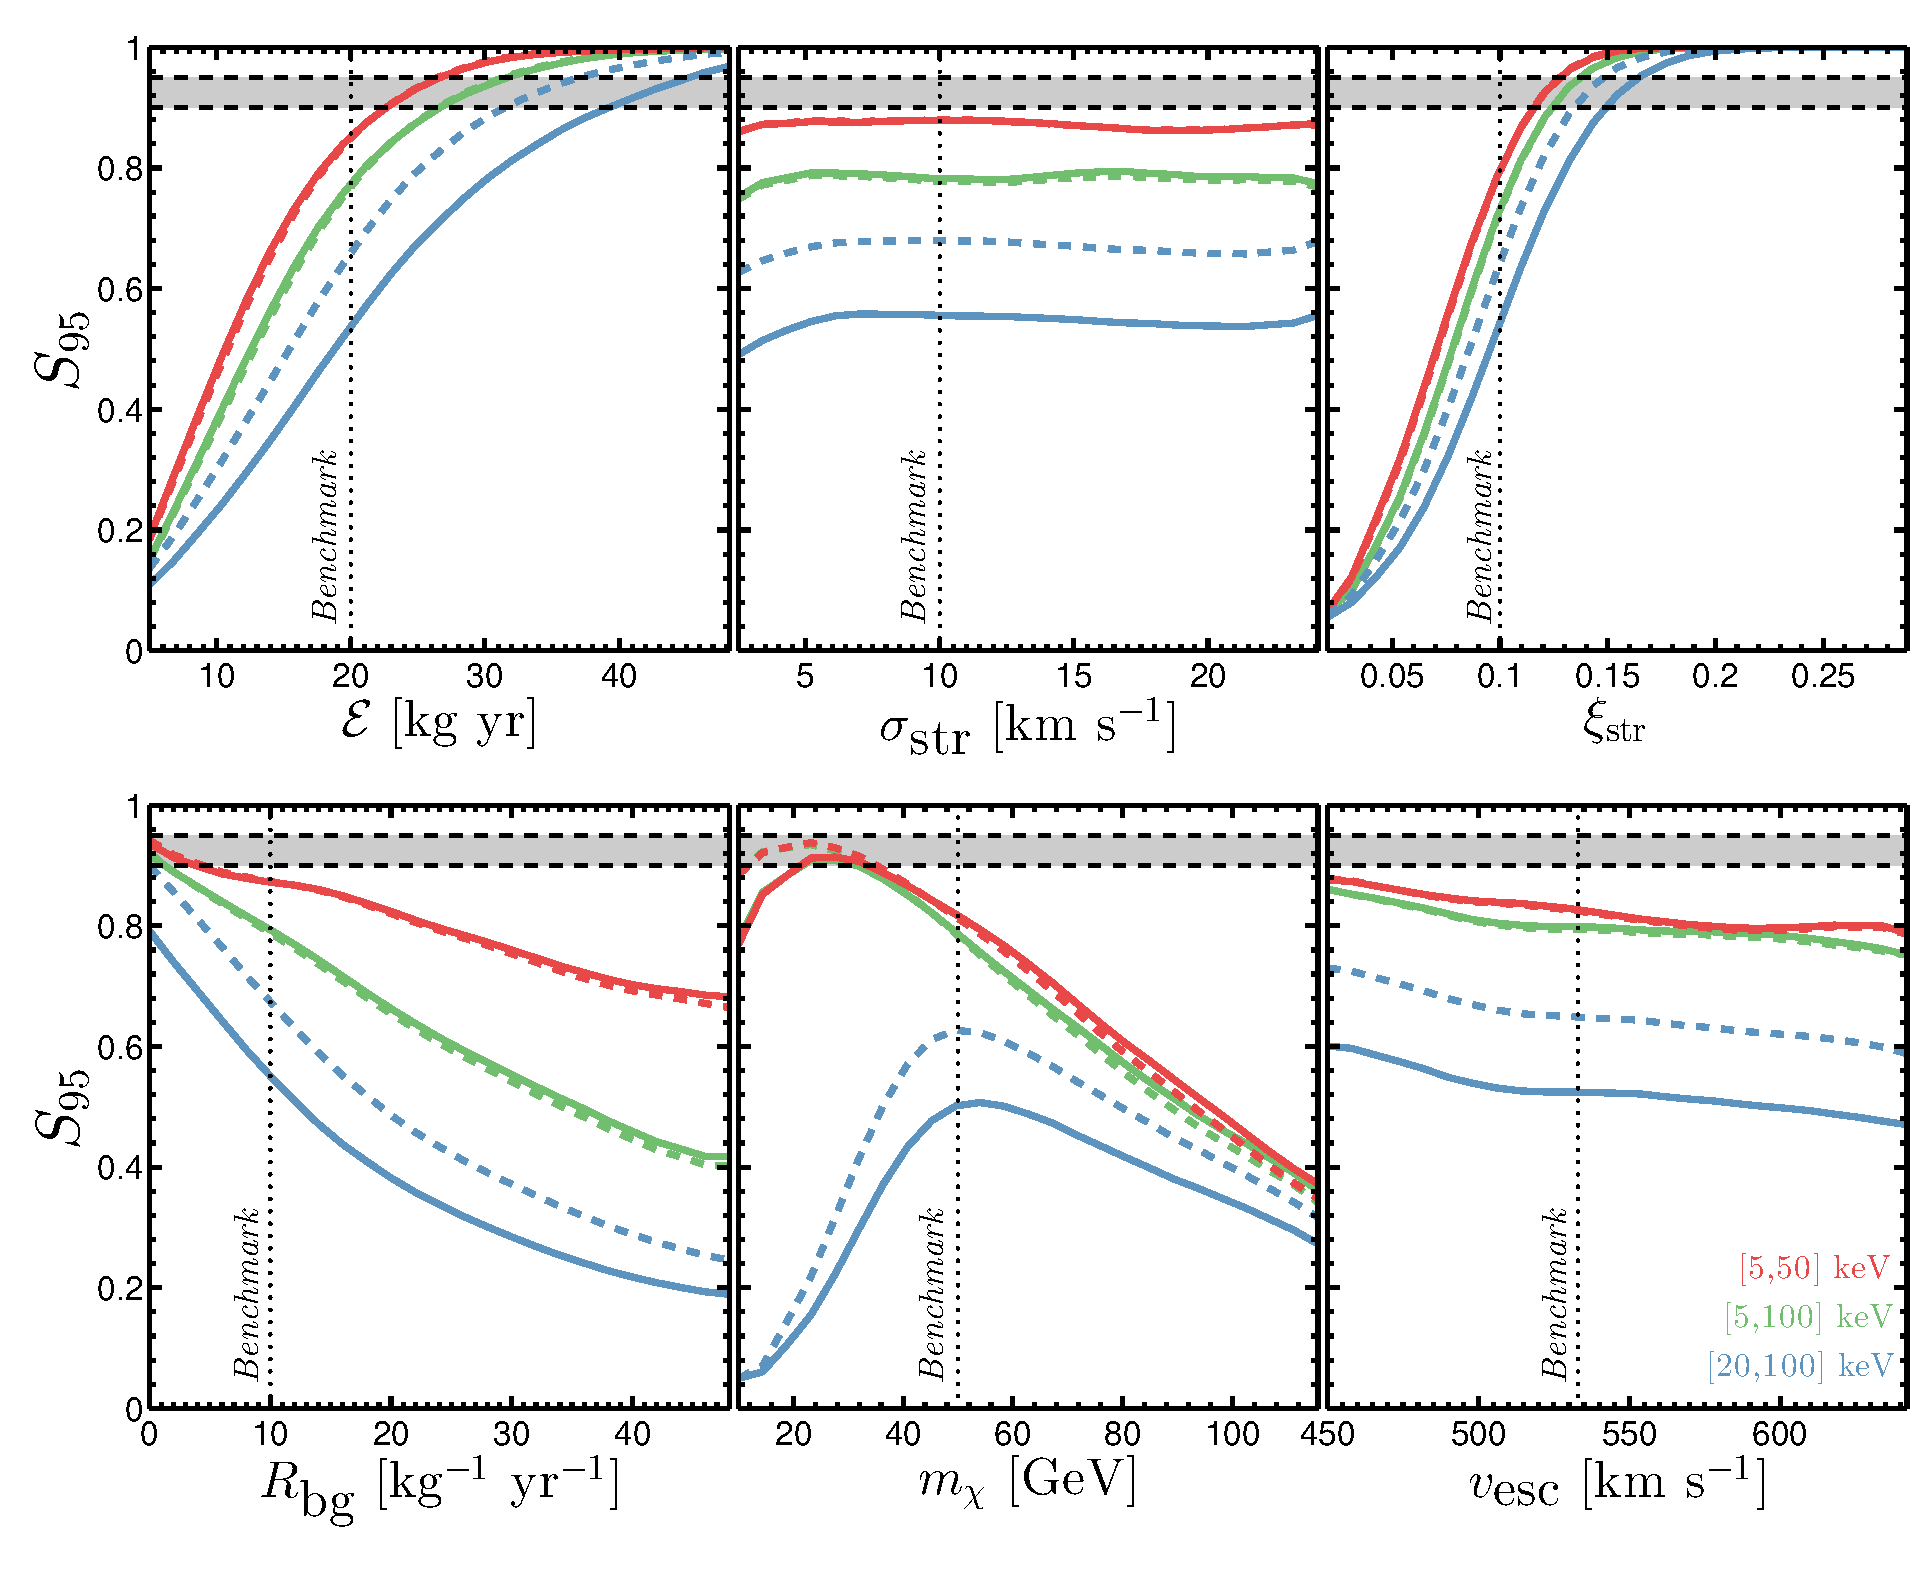
\includegraphics[trim = 0mm 0mm 0mm 0mm, clip, width=0.98\textwidth]{Figures/testcompare_sagit.eps}
    \caption[Results of non-parametric tests as a function of input parameters]{Significance obtainable by 95\% of experiments as a function of exposure, stream dispersion, stream density fraction, background rate, WIMP mass and escape speed for the Median direction (solid lines) and Kuiper (dashed lines) tests under the Sagittarius stream. The results are shown for energy windows of $[5,100]$ keV (green), $[5,50]$ keV (red) and $[20,100]$ keV (blue). The dashed lines indicate the desired $0.9-0.95$ level and the dotted lines in each plot indicate the input parameter used in the neighbouring plots.}
    \label{fig:testcompare_sagit}
\end{figure}
We first establish the role of the parameters other than the stream speed and direction on the performance of the tests; for now we focus on the benchmark case of the Sagittarius stream. In Fig.~\ref{fig:testcompare_sagit} we plot $S_{95}$ using the Kuiper and median direction $\chi^2$ tests. We show how this quantity varies with exposure time, stream dispersion, stream density, escape speed, WIMP mass and experimental background rate. As will become clear a choice that is particularly influential on our results here is the energy sensitive window of the detector, i.e. the threshold and maximum analysis energies. We display results for three examples, $[5,100]$ keV, $[5,50]$ keV and $[20,100]$ keV.

These first results are reasonably intuitive, with longer exposure times or for streams that takes up a larger fraction of the local DM density the signal is stronger and hence the tests perform better. The number of WIMP recoils from the stream scales linearly with exposure time and stream density fraction hence the significance of the result scales as roughly the square root of those quantities. Experiments with larger background rates perform predictably poorly compared to those with fewer backgrounds to contaminate the WIMP signal. Note that the quoted value of $R_\textrm{bg}$ is the rate observed in the case $[5,100]$ keV, the value taken for the other ranges has been scaled to account for the smaller sensitive window. The dispersion of the stream has no effect on the performance of the test, this is because of how the WIMPs scatter into the same angular area independent of how dispersed the distribution of their velocities is. To detect the Sagittarius stream at 90 - 95\% confidence in 95\% of experiments, one would need exposures between 10 - 20 kg yr for stream densities of around $\xi_{\rm str} \sim 0.1$, however this is lower for larger values of $\xi_{\rm str}$. The performance of the tests also depends on $m_\chi$, due mainly to the variation in the total number of events. Finally, the significance achieved decreases weakly as the escape speed is increased. This is because increasing $\vesc$ doesn't affect the recoils from stream, but slightly increases the number of recoils from the smooth halo scattering above the threshold.


\begin{figure}
	\centering
	%trim option's parameter order: left bottom right top
	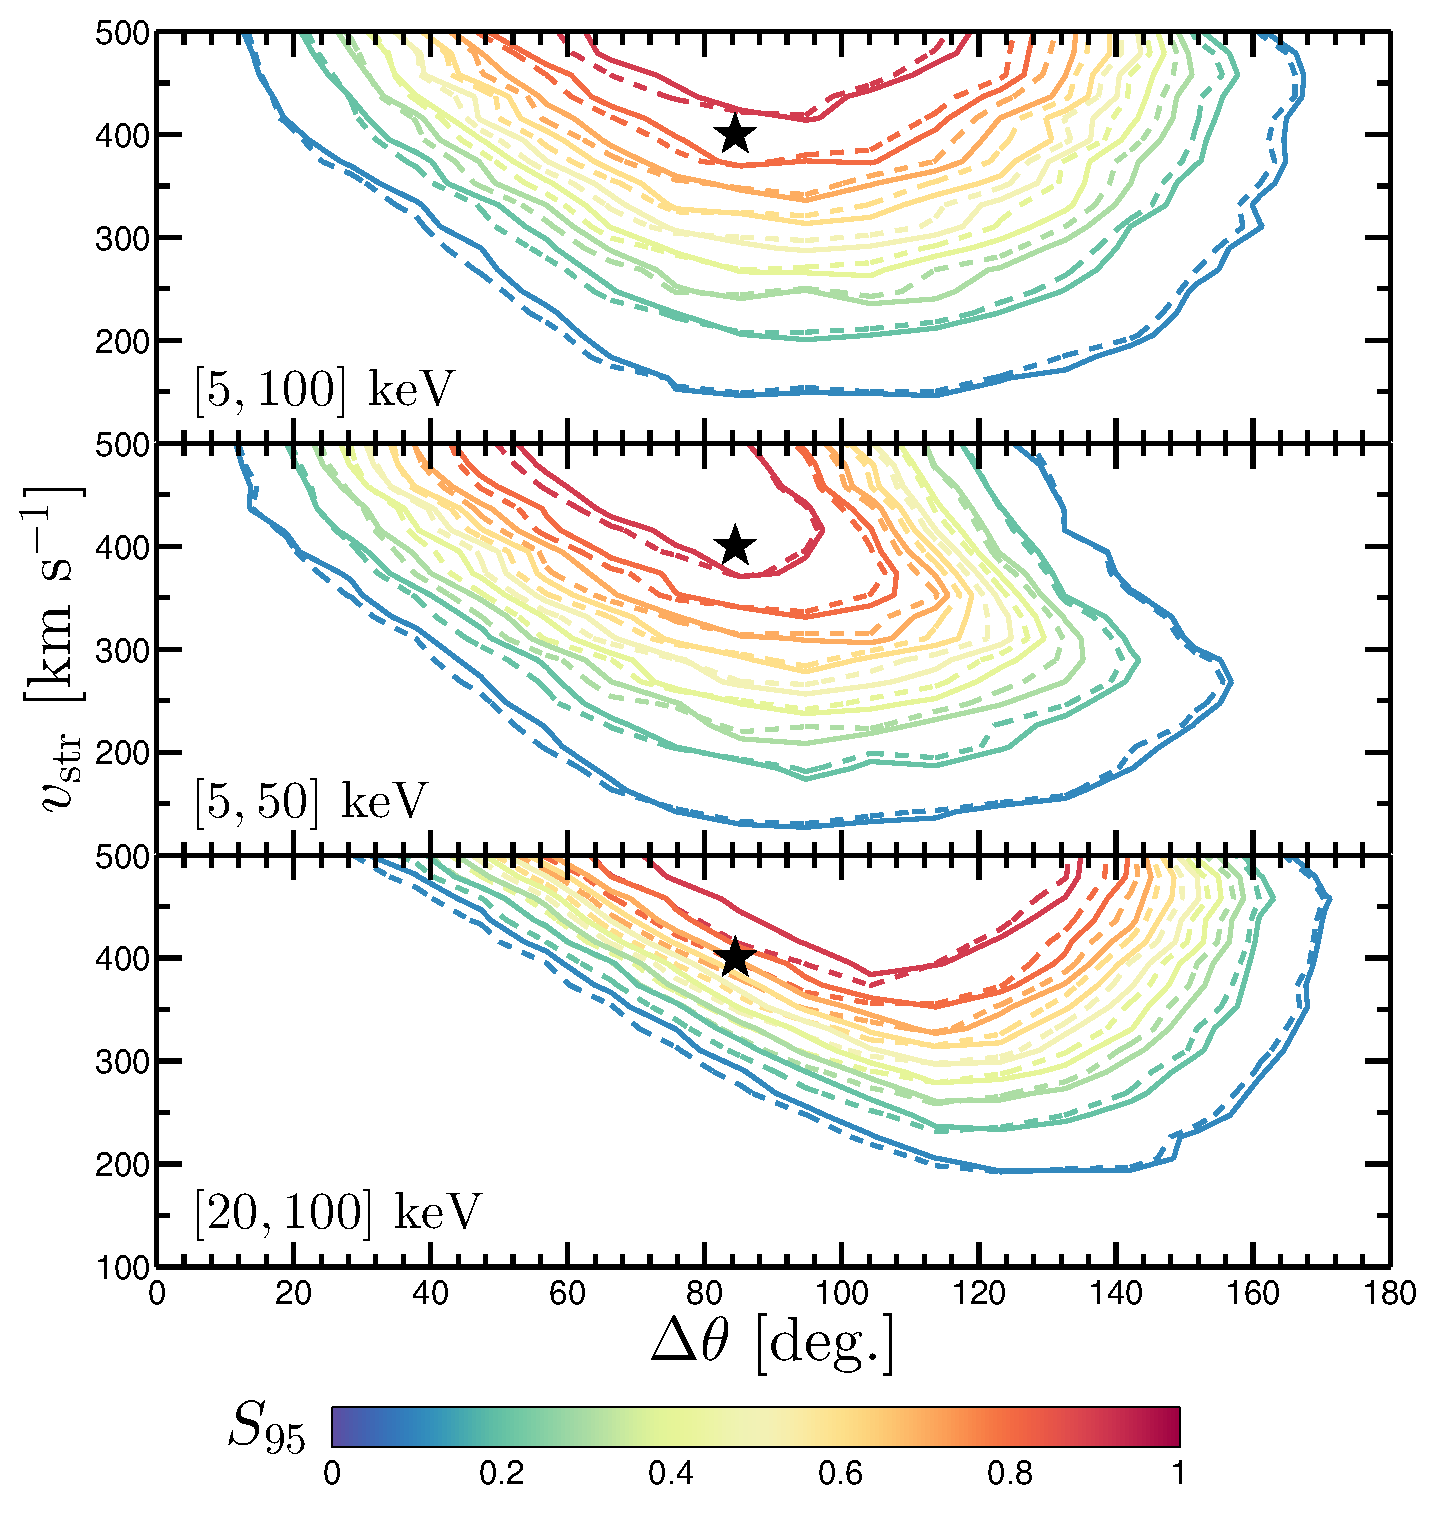
\includegraphics[trim = 0mm 0mm 0mm 0mm, clip, width=0.9\textwidth]{Figures/testcomparison_DeltaTheta_cont.eps}
	\caption[Non-parametric tests as a function of stream velocity]{Significance obtainable by 95\% of experiments over a 10 kg yr exposure as a function of stream speed and Galactic frame angle between stream direction and the lab velocity. The result for the Kuiper test is shown by the dashed lines and the median direction $\chi^2$ test by the solid lines. The three panels show the results for the three energy windows considered.}
	\label{fig:testcomparison_DeltaTheta}
\end{figure}
Having established the effect of the aforementioned parameter choices we will explore the detectability of general stream speeds and directions. For our results to be comprehensive the stream velocity need only be described by two parameters, the speed of the stream $v_\textrm{str}$ and the Galactic frame angle between the lab and stream velocities, $\Delta \theta$, defined in Eq.~(\ref{eq:deltatheta}). From symmetry arguments, changing the stream azimuthal angle with respect to $\textbf{v}_\textrm{lab}$ will not affect any of our results as it yields the same angular spectrum up to a rotation. Figure \ref{fig:testcomparison_DeltaTheta} shows how the significance varies with stream direction and speed, as well as the dependence on the energy window of the detector. The tests do not perform equally well over the range of stream directions. In particular the tests return a low significance when the stream is anti-aligned with the lab velocity as in this case the hypotheses of rotational symmetry and median direction are correct and the distribution of the statistics reverts to that of the null case. The other important contribution to the significance of the test result is from the number of observed stream recoils which for small $\Delta\theta$ is very low and for slower streams or high threshold energies as low as 0. The symmetry in the plots is due to this dependence on both the sample size and the positioning of the stream recoils with respect to the background halo recoils. One can also see that for the fastest streams, increasing the threshold energy results in a higher value of significance, this can be attributed to what is essentially a background rejection effect, whereby removing some of the low energy halo recoils the stream appears stronger in the signal, even with fewer overall events. The drop-off at large $\Delta\theta$ in the case of the 50 keV maximum energy is due to the stream recoils falling above the energy window, which is the reverse effect as at low values of $\Delta\theta$ in the case when the threshold has been increased to 20 keV.

A weakness of the Kuiper and median direction tests are that they exploit the direction information of the recoils only; the use of the recoil energy as well as the directional information is desirable. It may be possible to include the energy dependence of the signal by performing the test successively on energy ordered recoils or by binning the recoils in energy. In the case where there is no stream present the hypotheses of rotational symmetry and median direction are satisfied for all energies. However with a stream in the signal there will be a range of energies where the hypothesis is not satisfied. The degree to which the test is failed will increase for larger energies and then above a certain value of energy set by the stream speed, the test returns a value closer to the null case. Accounting for this effect in the test statistic would decrease the overlap between the null and alternative distributions and hence increase the significance of a particular result. However it is likely to be a small effect, as we showed in Fig~\ref{fig:polar}, the enhancement in the recoil energy spectrum induced by a stream is very slight. Furthermore dividing the recoils up in energy would result in a loss in information for each individual evaluation of the test statistic, so we expect the tests to perform on par or worse than without the energy information for low numbers of recoils. A more powerful method of including the energy dependence of the signal is with a likelihood fit.





\subsection{Likelihood analysis}\label{sec:directional_likelihood}
We turn our attention now towards a statistical test capable of placing constraints on the properties of the stream as well as testing for its existence. First we require a likelihood function. There are 11 free parameters in our model, $\boldsymbol{\theta} = \lbrace m_\chi, \sigma^{\rm SD}_p, \rho_0, \sigma_v,v_\textrm{esc},\sigma_\textrm{str},\textbf{v}_{\rm str},\xi_{\rm str},R_\textrm{bg}\rbrace$, where we split the velocity of the stream into its three Galactic coordinate components. We define the likelihood function as the product of the probabilities for obtaining recoils located at $(E_r^i,\hat{\textbf{q}}^i)$ ($i = 1, ..., N_{\rm obs}$) multiplied by a Poisson factor accounting for the probability of obtaining $N_{\rm obs}$ observed events given an expected number $N_{\rm exp}(\boldsymbol{\theta})$,

\begin{equation}
	\mathscr{L}(\boldsymbol{\theta})= \frac{N_{\rm exp}^{N_{\rm obs}}}{N_{\rm obs} !} e^{-N_{\rm exp}} \times\prod_{i=1}^{N_{\rm obs}} \bigg[\lambda P_\textrm{wimp}(E_r^i,\hat{\textbf{q}}^i) + (1-\lambda)P_\textrm{bg}(E_r^i)\bigg] \nonumber. 
\end{equation}
The expected number of events is a function of the parameters $\boldsymbol{\theta}$ and defined as, 
\begin{eqnarray}
	N_{\rm exp} &=& N_{\rm exp}^{\textrm{wimp}} + N_{\rm exp}^{\textrm{bg}} \\ &=& \mathcal{E} \left[ \int_{E_\textrm{th}}^{E_\textrm{max}} \int_{\Omega_r} \frac{\textrm{d}^2R}{\textrm{d}E_r \textrm{d}\Omega_r}\, \textrm{d}\Omega_r \, \textrm{d}E_r+ R_\textrm{bg}\right].
\end{eqnarray}
The probabilities $P_\textrm{wimp}$ and $P_\textrm{bg}$ are the probabilities for an event to occur at $(E_i,\hat{\textbf{q}}_i)$ in the signal and background (no WIMP) cases respectively, i.e.
\begin{eqnarray}
	P_\textrm{wimp}(E^i_r,\hat{\textbf{q}}^i; \boldsymbol{\theta}) &=& \frac{1}{R} \frac{\textrm{d}^2 R}{\textrm{d}E_r\textrm{d}\Omega_r}\bigg|_{E_r^i,\hat{\textbf{q}}^i; \boldsymbol{\theta}} \\
	P_\textrm{bg}(E_r^i) &=& \frac{1}{4\pi R_{\rm bg}} \frac{\textrm{d}R_{\rm bg}}{\textrm{d}E_r}.
\end{eqnarray}
The background probability  distribution we assume is isotropic with an exponentially falling recoil spectrum $\textrm{d}R_{\rm bg}/\textrm{d}E_r \propto \exp\left(-E_r/17.5\,{\rm keV}\right)$ where 17.5~keV is chosen to mimic the slope of the recoil energy spectrum of a 50 GeV WIMP in a fluorine experiment. We sum the signal and background distributions weighted by the signal fraction $\lambda$ defined as,
\begin{equation}
  \lambda = \frac{N_{\rm exp}^\textrm{wimp}}{N_{\rm exp}} \, .
\end{equation}
The parameter that will always be poorly recovered in this analysis is $v_\textrm{esc}$, as its effect on the recoil energy spectrum is very small and usually only becomes important at energies beyond the maximum set for directional detectors. We can overcome this issue by treating $v_\textrm{esc}$ as a nuisance parameter and account for its uncertainty by hand by including an additional term to the likelihood in the form of a Gaussian with mean and standard deviation of $v_\textrm{esc} = 533\, \pm \, 54$ km s$^{-1}$ \cite{Piffl:2013mla}. We then multiply the original likelihood by this Gaussian function.

The WIMP density, $\rho_0$, and cross section, $\sigma^{\rm SD}_p$, will also be problematic as they only control the amplitude of the recoil spectrum and hence only the number of events seen for a given exposure. Even for the rather large stream densities that we are considering here the difference between the number of events seen in the stream case compared with the null case is small. Moreover, the two parameters are degenerate with one another meaning there is no single set of values for $\rho_0$ and $\sigma^{\rm SD}_p$ that maximise the likelihood function in its current form. So we also adopt a Gaussian parameterisation for $\rho_0$ at the correct value. We choose a mean and standard deviation that reflect the current observational constraints on the local density, $\rho_0 = 0.3 \, \pm \, 0.1$ GeV cm$^{-3}$ \cite{Read:2014qva}.

\begin{figure}
	\centering
	%trim option's parameter order: left bottom right top
	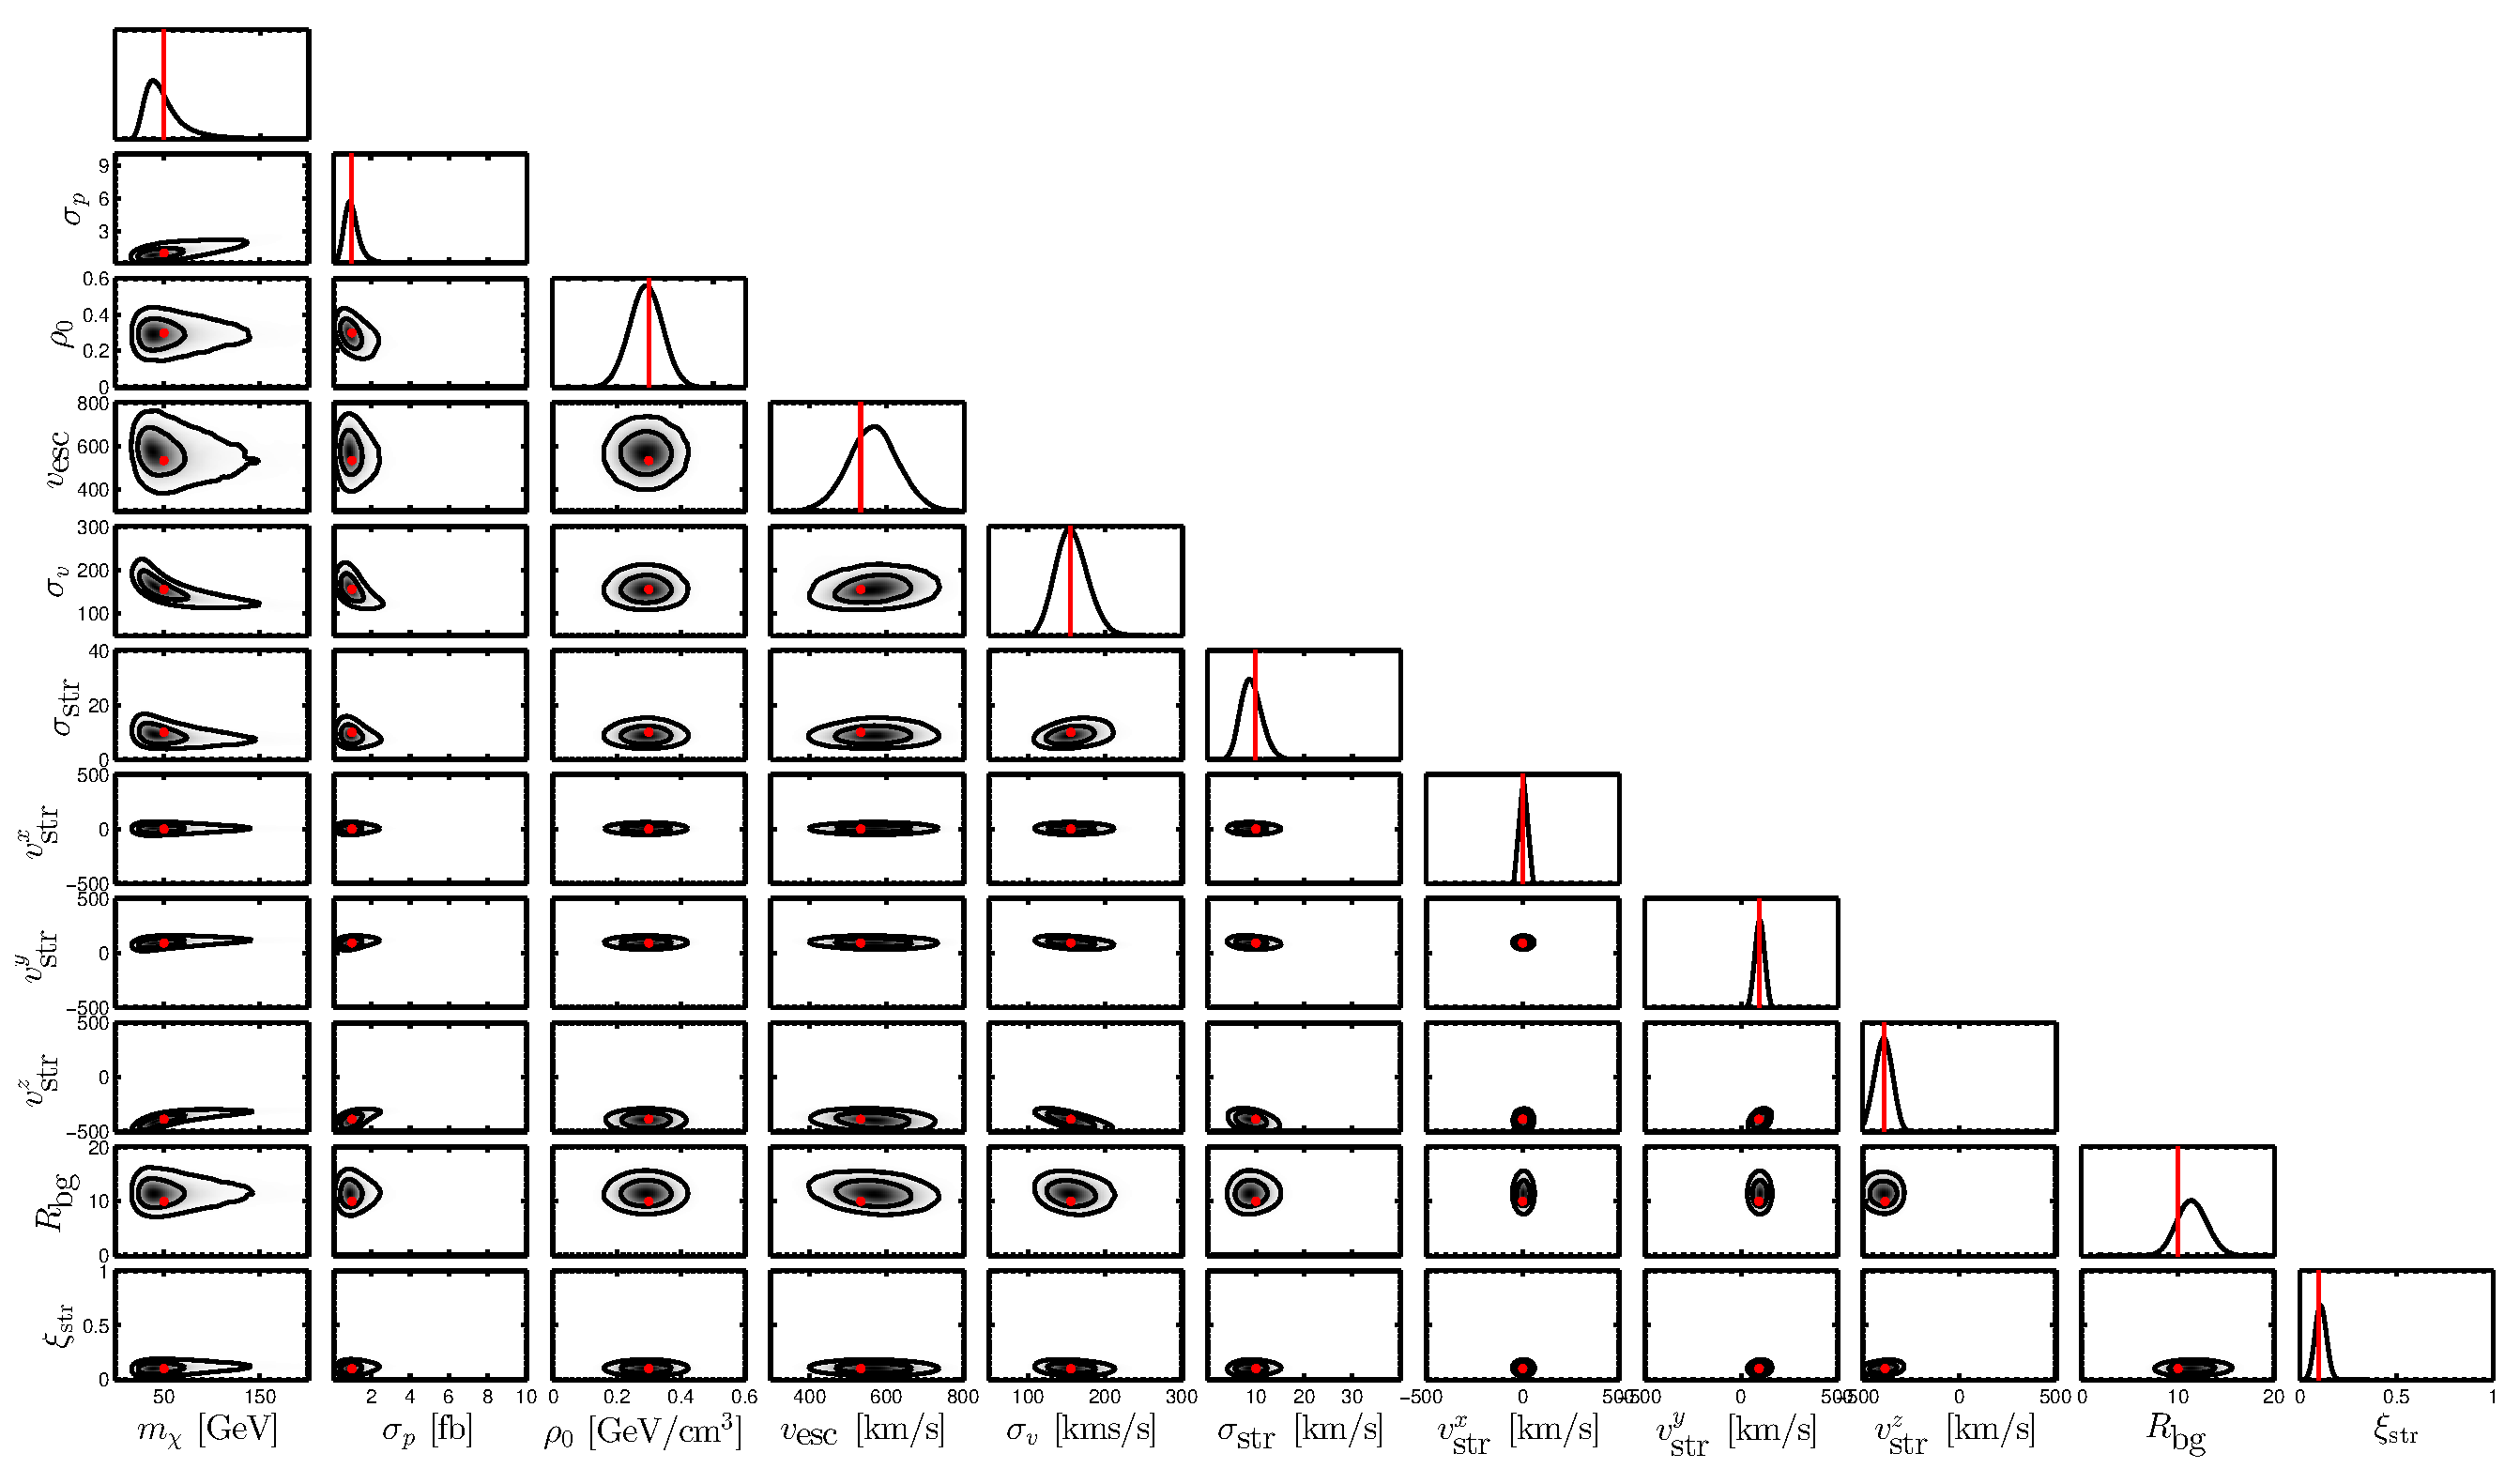
\includegraphics[trim = 0mm 0mm 0mm 0mm, clip, width=1.5\textwidth,angle=90]{Figures/posts_11params.eps}
	\caption[Triangle plot for reconstructed parameters of the SHM+Str model]{Triangle plot for reconstructed parameters of the SHM+Str model. The contours indicate the 68\% and 95\% confidence regions. The red dots/lines indicate the location of the input parameters.}
	\label{fig:posts_11params}
\end{figure}
First we will attempt to reconstruct the parameters of this model including the stream properties using the benchmark set of inputs. To do this we sample the likelihood over the full available parameter space with the nested sampling software \textsc{Multi}N\textsc{est} \cite{Feroz:2013hea, Feroz:2008xx} using 5000 live points, an evidence tolerance factor of 0.05 and sampling efficiency of 0.3. We then calculate 1-d (2-d) 68\% and 95\% confidence intervals (contours) using the asymptotic properties of the profile likelihood~\cite{Cowan:2010js}. The triangle plot of Fig.~\ref{fig:posts_11params} shows the parameter reconstructions in relation to the input values. The stream parameters, by virtue of being unconnected to the other halo parameters, are recovered well. The main source of uncertainty stems from the SHM and WIMP parameters, in particular $m_\chi$. The effect of the Gaussian parameterisation of $v_\textrm{esc}$ and $\rho_0$ is apparent and equivalent to using a Gaussian prior. There is a still some correlation in the $\rho_0-\sigma_p$ plane but the degeneracy has been broken. The halo parameters are reconstructed less accurately if they are not treated with a Gaussian function in the likelihood, however this parameterisation is representative of existing astrophysical measurements. This example shows that good constraints could be made on the parameters describing a stream if the correct model is used in constructing the likelihood function for the data. Importantly, we note that the exposure times needed to make these constraints  $\sim 5$ kg yr are significantly shorter than are needed when the non-parametric directional tests are used.

In analogy with the methodology of Sec.~\ref{sec:directional_nonparametric} we can use our likelihood function to develop a test for the existence of a stream in the data.  
An appropriate test involves the profile likelihood ratio statistic as it is based on the assumption that the null hypothesis is recovered by applying a constraint to a more general alternative hypothesis. A version of this test is often used to calculate WIMP discovery limits on the mass-cross section parameter space and will appear again in Chapter~\ref{chapter:nufloor}. Although here instead of testing for the presence of a WIMP over some background, rather we are testing for the existence of a stream in some already confirmed WIMP events.

We define the null hypothesis $H_0$ to be the SHM model and the alternative, $H_{\rm str}$, to be the SHM+Str model. The null hypothesis is then recovered with the same likelihood function under the constraint $\xi_{\rm str} = 0$. The likelihood ratio between the null and alternative hypotheses is,
\begin{equation}
	\Lambda = \frac{\mathscr{L}(\hat{\hat{\boldsymbol{\theta}}}, \xi_{\rm str} = 0)}{\mathscr{L}(\hat{\boldsymbol{\theta}} )} \, ,
\end{equation}
Where $\hat{\boldsymbol{\theta}}$ are the maximum likelihood estimators in the alternative model, and $\hat{\hat{\boldsymbol{\theta}}}$ are the maximum likelihood estimators evaluated when $\xi_{\rm str} = 0$. The likelihood ratio test statistic is then defined,
\begin{equation}
	\mathcal{D} = \left\{ \begin{array}{rl}
	-2\ln \Lambda  & \, \, 0\le \hat{\xi}\le1 \,,\\
	0  & \, \, \hat{\xi}<0, \, \, \hat{\xi}>1 \,.
	\end{array} \right. 
\end{equation}

Next we require a definition for the statistical significance of a particular test result. This requires knowledge of how the profile likelihood ratio test statistic $\mathcal{D}$ is distributed in the case that the null hypothesis is true, i.e. if the observed value is $\mathcal{D}_\textrm{obs}$
\begin{equation}
	S = \int_0^{\mathcal{D}_\textrm{obs}} f(\mathcal{D} | H_0) \, \textrm{d}\mathcal{D} \,.
\end{equation}
It is known however from Wilks' theorem \cite{Cowan:2010js} that the distribution of the profile likelihood ratio test statistic in the null case asymptotes towards a half $\chi_1^2$ distribution. Hence the discovery significance is defined as $S = \textrm{erf}\left(\sqrt{\mathcal{D}_\textrm{obs}/2}\right)$. However as we will be computing quite high values of significance it is simpler to deal in units of standard deviation, $\sigma$, i.e. $S = \sqrt{\mathcal{D}_\textrm{obs}}$. So a value of $\mathcal{D}_\textrm{obs} = 1$ corresponds to a 1$\sigma$ result or a significance of 68\%. The significance obtainable by 95\% of mock experiments, $S_{95}$, is then found by first building the distribution $f(\sqrt{\mathcal{D}})$ by applying the test on many Monte Carlo generated datasets containing a stream, and then solving the equation,
\begin{equation}
\int_0^{S_{95}} f(\sqrt{\mathcal{D}})\textrm{d}\sqrt{\mathcal{D}} = 0.95 \, .
\end{equation}

As in the previous Section, we demonstrate the performance of the test over a range of stream velocities where we again use the parameters $\Delta \theta$ and $v_\textrm{str}$ to describe the stream velocity. In Fig. \ref{fig:S95_DeltaTheta} we plot significance in units of $\sigma$ obtainable by 95\% of hypothetical experiments using the profile likelihood ratio test as a function of stream speed, $v_\textrm{str}$, and direction given by $\Delta \theta$, for the three energy windows considered. For comparison, in Fig. \ref{fig:N_wimp_str_location_cont} we plot the number of WIMPs originating in the stream, $N_\textrm{wimp}^\textrm{str}$, where we have split the observed events into stream and SHM recoils,
\begin{equation}
  N_\textrm{wimp} = N_\textrm{wimp}^\textrm{Str} + N_\textrm{wimp}^\textrm{SHM} \, .
\end{equation}

\begin{figure}
  \centering
  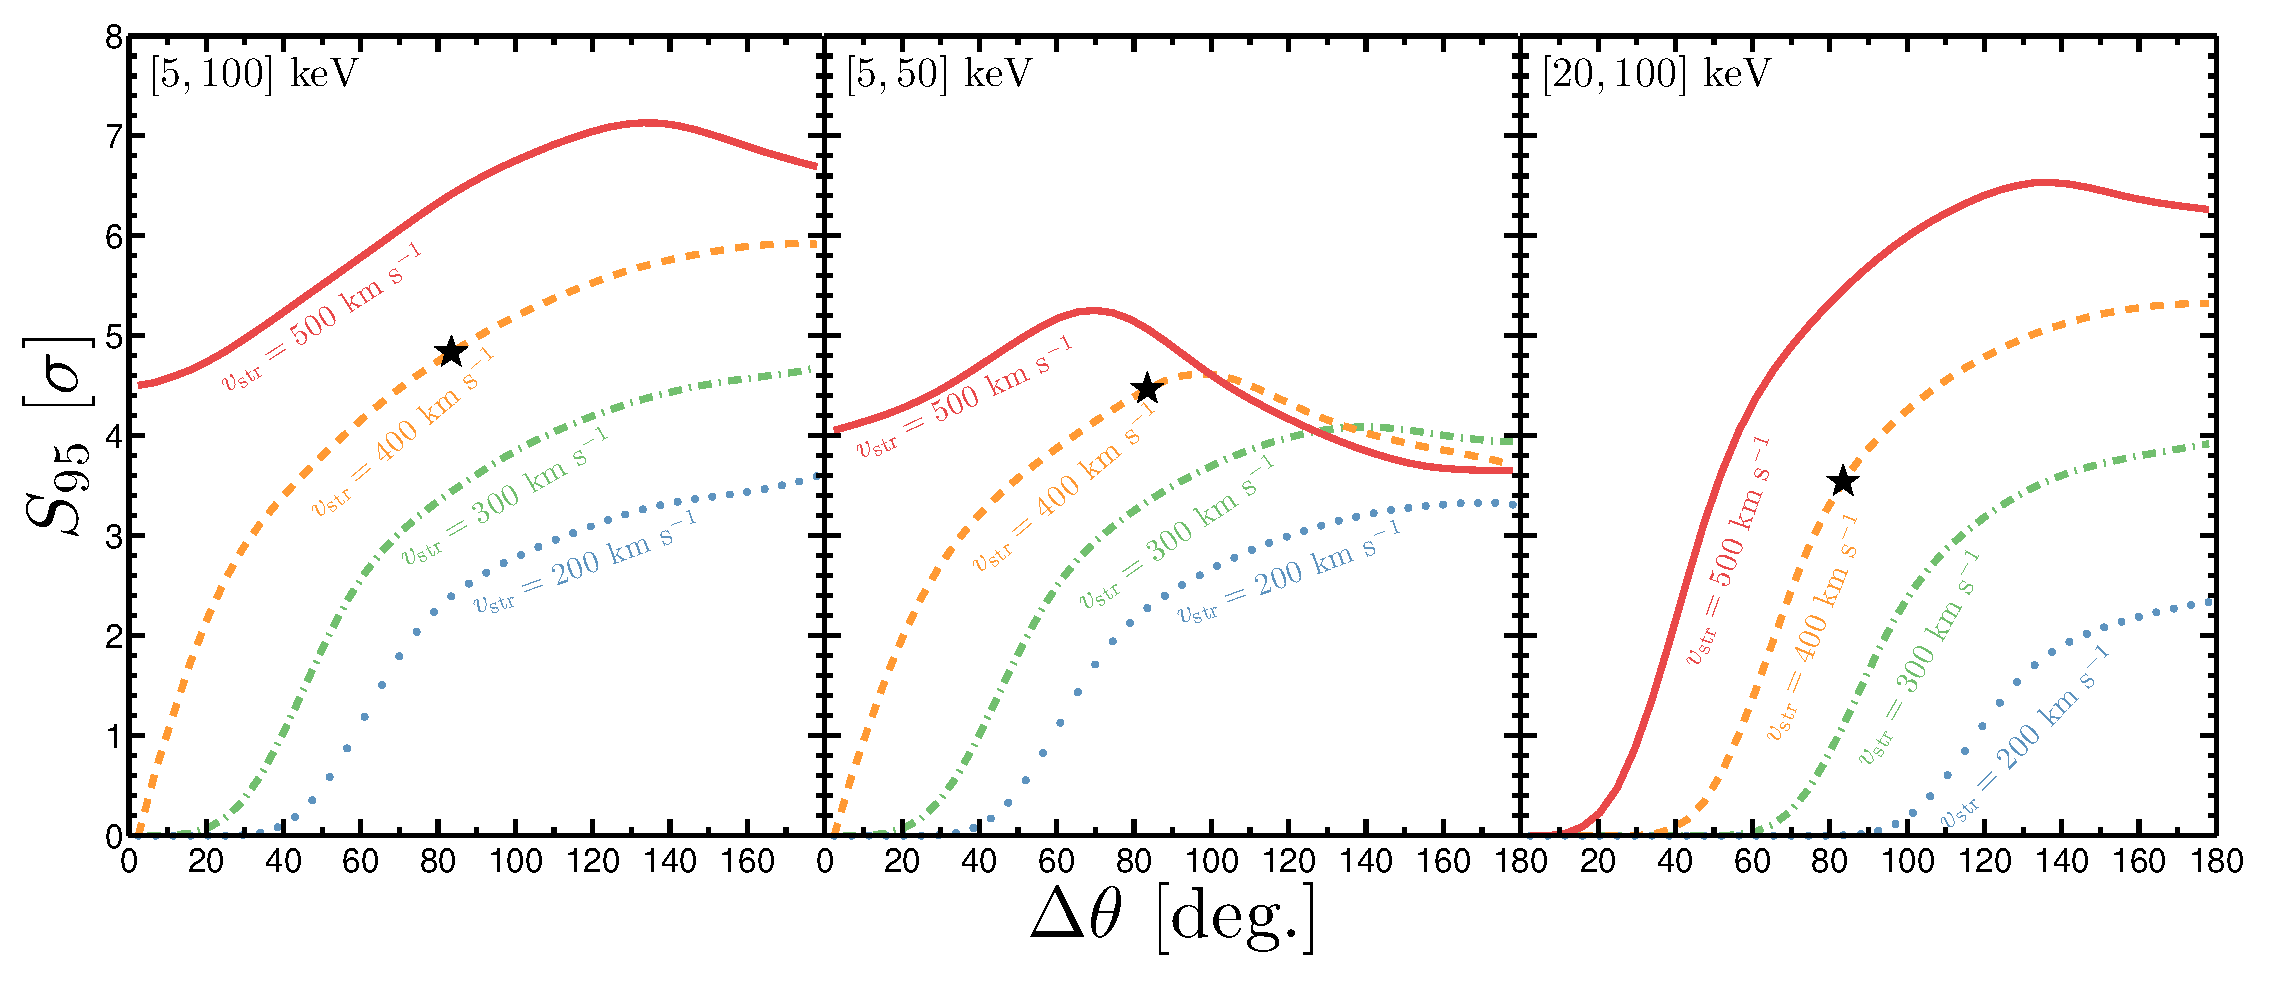
\includegraphics[trim = 0mm 0 0mm 0mm, clip, width=0.98\textwidth]{Figures/S95_DeltaTheta.eps}
  \caption[Profile likelihood test significance as a function of stream angle]{Significance achievable in 95\% of experiments in units of $\sigma$ using a profile likelihood ratio test. The test result is shown as a function of angle between lab and stream velocities. The curves correspond to, from top to bottom, $v_\textrm{str} = 500$ km s$^{-1}$ (red solid line), 400 km s$^{-1}$ (orange dashed), 300 km s$^{-1}$ (green dot-dashed), and 200 km s$^{-1}$ (blue dotted). The speed and direction of the Sagittarius stream example is indicated with a black star.}
  \label{fig:S95_DeltaTheta}
\end{figure}
\begin{figure}
  \centering
  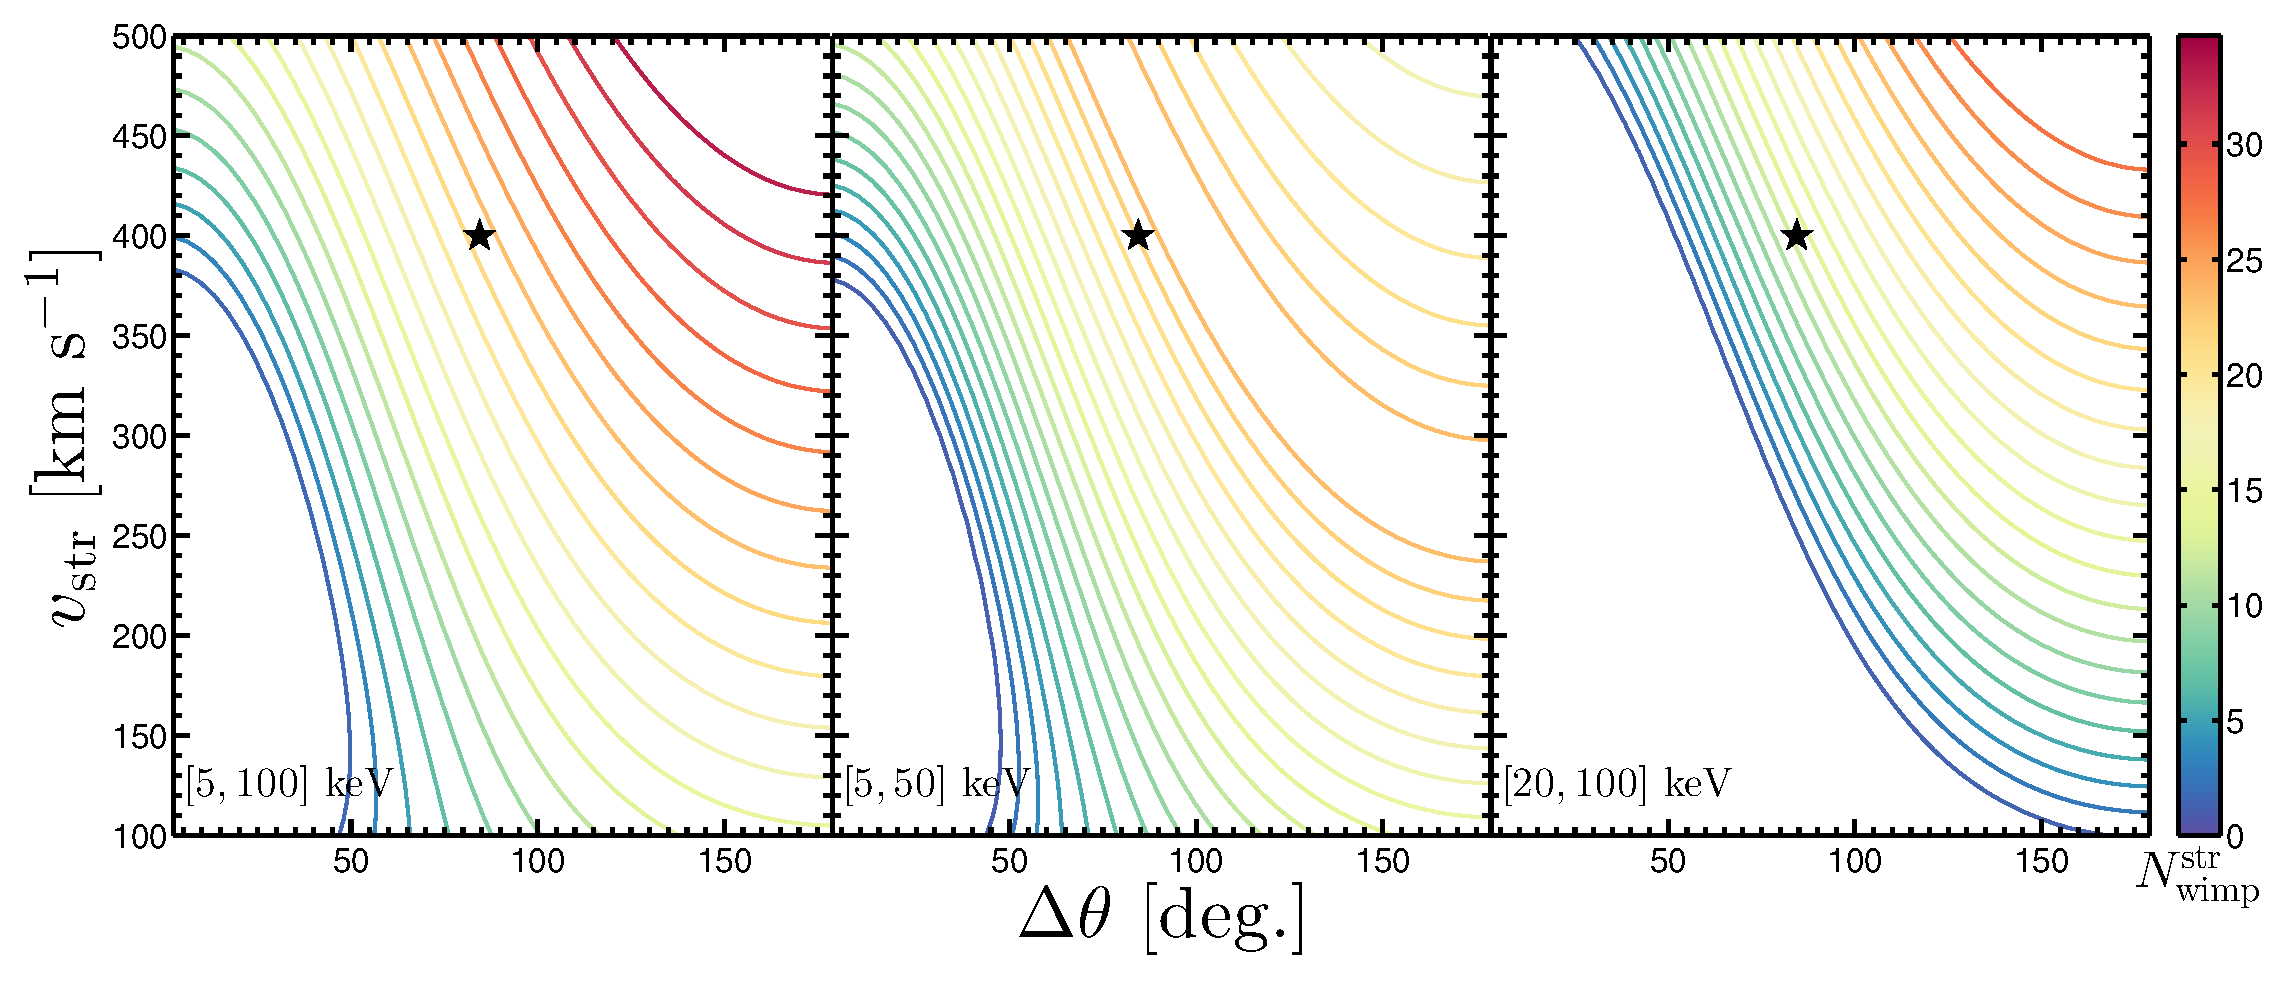
\includegraphics[trim = 0mm 0 0mm 0mm, clip, width=0.98\textwidth]{Figures/N_wimp_str_location_cont.eps}
  \caption[Number of stream recoils as a function of stream velocity]{Number of stream recoils as a function of stream speed, direction and for three energy sensitive windows (left to right panels). The speed and direction of the Sagittarius stream example is indicated with a black star.}
  \label{fig:N_wimp_str_location_cont}
\end{figure}
In Figs.~\ref{fig:S95_DeltaTheta} and \ref{fig:N_wimp_str_location_cont} the parameter values not displayed are fixed at the benchmark values used in Fig.~\ref{fig:testcompare_sagit}, with the exception of exposure which we now reduce to 5~kg~yr. The tests by virtue of being parametric perform much more powerfully than the non-parametric tests. The enhancement in performance can also be attributed to the use of the full energy and direction data whereas before only the direction information was used. Furthermore the tests achieve high significance over a wide range of stream velocities, with the limiting factor being the number of WIMPs coming from the stream, $N_\textrm{wimp}^{\textrm{str}}$, as can be seen by comparing the two Figures. For low values of $\Delta\theta$ when the number of stream WIMPs drops to 0, the significance can be seen to do likewise. There is similarly a dependence on the energy window of the detector which causes a reduction in the number of stream WIMPs when a portion of the stream recoils are excluded by the maximum of the energy window. This can be seen in the middle panels when the curves begin to decrease for large $\Delta \theta$. However the significance for faster stream speeds is enhanced over what might be expected simply from looking at $N_\textrm{wimp}^\textrm{str}$. This can be attributed to faster streams becoming more prominent in the signal due to the exponential drop off with energy of the event rate for the background halo.

\subsection{Discussion}
Using both non-parametric directional tests and a profile likelihood test, we have shown that there are reasonable prospects for the detection of a moderately high density tidal stream by a future directional detector. We began with the fixed example of a Sagittarius-like stream and then explored the dependence on the parameters of the stream, namely its speed, direction, dispersion and density. Using non-parametric directional statistics the detection of a Sagittarius-like stream would need a total of around 900 events, but with a likelihood fit good constraints can be placed on the stream parameters with around 300 events.

The advantage of using non-parametric tests is that one need not assume a model to describe the data, simply that the data satisfy either a null or alternative hypothesis. The advantage of the tests we exploit here is that they are constructed rather generally and the basic hypotheses are relatively simple. However non-parametric tests will always return a less significant result than parametric tests. The likelihood analyses also make use of both the energy and direction information of the recoils whereas the non-parametric tests are direction only. The disadvantage of the likelihood approach however is that we must pick a specific model to describe the substructure that one predicts to be present in the data. We now explore possible ways of making claims about the presence of non-Maxwellian structure in the halo in a parametric way that does not require particular choices for the functional form describing it.

\section{Reconstructing the velocity distribution}\label{sec:directional_reconstruction}
We now move to more model independent methods for measuring properties of the local velocity distribution. This will involve extending a general parameterisation of the {\it speed} distribution used in the analysis of standard direct detection data~\cite{Peter:2011eu,Kavanagh:2013wba}, to the fitting of the {\it velocity} distribution with directional data. There have been long-standing attempts to devise methodologies for handling astrophysical uncertainties in direct detection experiments, see e.g. Refs.~\cite{Fox:2010bz,Fox:2010bu,Frandsen:2011gi,Gondolo:2012rs,DelNobile:2013cta,Fox:2014kua,Feldstein:2014gza,Anderson:2015xaa,Gelmini:2016pei,Kahlhoefer:2016eds}. In the context of directional detection experiments the situation is more complicated as the angular recoil spectrum is much more sensitive to the values of the underlying astrophysical parameters. One must also consider the full 3-dimensional velocity distribution rather than the 1-d speed distribution and as such requires a suitable angular basis for the parameterisation. Past attempts to develop astrophysics independent methods for directional detection have involved decomposing the velocity distribution into integrals of motion~\cite{Alves:2012ay}, or spherical harmonics~\cite{Lee:2014cpa}.

Following the formalism introduced in Ref.~\cite{Kavanagh:2015aqa} we test a discretised approach for empirically parameterising the velocity distribution. The velocity distribution is divided into angular bins, each described by an empirical 1-d speed distribution which does not vary with angle over the bin. The goal now is to use mock data and likelihood fits to test the accuracy of the reconstructed WIMP signal using this empirical method compared with model-dependent fits. We also consider both energy only and directionally sensitive direct detection experiments to quantify the advantages of introducing angular information. We compare reconstructions of the WIMP mass, cross section and velocity distribution in three distinct cases: A) when the velocity distribution is known exactly; B) when the general functional form of the distribution is known (as in the previous Section); and C) when no assumptions are made about the velocity distribution. We test these three methods on the three benchmark velocity distributions defined in Chapter~\ref{chapter:direct}, the SHM, the SHM+Stream and the SHM+Debris Flow. 

As before we continue to fix our results at a single particle physics benchmark with a mass of $m_\chi = 50 \, \, \mathrm{GeV}$ and a solely SD cross section of $\sigma^{\rm SD}_p = 10^{-39} \, \, \mathrm{cm}^2$. We extend beyond the experimental setup introduced before to the combination of two experiments with xenon and fluorine targets. This allows us to explore the complementarity of multiple targets but also allows us finer control in the level of directional information used. We will consider cases in which neither experiment has directional sensitivity, in which only one of the experiments has directional sensitivity and in which both experiments are directionally sensitive. 

Our choice of a xenon target detector is inspired by projections for the next generation of ton-scale liquid xenon experiment such as LZ~\cite{Akerib:2015cja} and Xenon1T~\cite{Aprile:2015uzo}. Although these experiments are not designed with any directional sensitivity they represent a useful and realistic benchmark for an exposure and threshold ($\sim 5\,\textrm{keV}$) that can be expected in the next generation of direct detection experiments. Though as we discussed earlier there are tentative suggestions that it may be possible to extract directional information in liquid xenon experiments with columnar recombination~\cite{Nygren:2013nda,MuAaoz:2014uxa,Li:2015zga,Mohlabeng:2015efa}. The choice of a fluorine detector is the same as in the previous Section, inspired by existing low pressure gas TPCs with CF$_4$. For these results we set a modest threshold of 20 keV, in line with what is currently achievable~\cite{Leyton:2016nit}. A summary of the parameters used for each experiment and the number of events observed for each halo model are given in Table~\ref{tab:benchmarks}. 


\begin{table}[t]\centering
\ra{1.3}
\begin{tabularx}{\textwidth}{c|YYY|YYY}
\hline\hline
Target	& $E_\mathrm{th}$/keV	& $E_\mathrm{max}$/keV & $\mathcal{E}$/kg yr & $N_\mathrm{events}^{\mathrm{SHM}}$ & $N_\mathrm{events}^{\mathrm{SHM+Str}}$& $N_\mathrm{events}^{\mathrm{SHM+DF}}$ \\
\hline
Xe & 5 & 50 & 1000 & 878 & 922 & 893 \\
F   & 20 & 50 & 10 & 50 & 67 & 64 \\
\hline \hline
\end{tabularx}
\caption[Parameters for the two mock experiments]{Parameters for the two mock experiments considered in this Section: threshold energy $E_\mathrm{th}$, maximum analysis energy $E_\mathrm{max}$ and exposure $\mathcal{E}$. Also shown are the number of expected events in the both experiments for each of the three astrophysical benchmark models.}
\label{tab:benchmarks}
\end{table}

We compare the reconstruction of the WIMP and velocity distribution parameters made using three methods each with a different level of a priori knowledge assumed.
\begin{itemize}
\item{{\bf Method A: Perfect knowledge.} This is the best case scenario when both the functional form and parameter values of the velocity distribution are known exactly. The parameters that are reconstructed with this method are only $\{m_\chi,\sigma_p^{\textrm{SD}}\}$ for all three halo models.}

\item{{\bf Method B: Functional form known.} In this case the functional form of the velocity distribution (i.e. SHM, SHM+Str or SHM+DF) is known, however the parameter values are not. The number of parameters reconstructed with this method varies depending on the chosen halo model. In the case of the SHM there are 4 parameters: $\{m_\chi,\sigma_p^{\textrm{SD}},v_0,\sigma_v\}$. For the SHM+Str model (in a slight simplification from Sec.~\ref{sec:directional_nonparametric}) there are 9 parameters: $\{m_\chi,\sigma_p^{\textrm{SD}},v_0,\sigma_v,\sigma_{\rm str},\mathbf{v}_{\rm str},\xi_{\rm str}\}$, and for the SHM+DF model there are 6 parameters: $\{m_\chi,\sigma_p^{\textrm{SD}},v_0,\sigma_v,v_f,\xi_{\rm DF}\}$.}

\item{{\bf Method C: Empirical parameterisation.} With this method no knowledge is assumed about the form or parameters of the underlying velocity distribution. We fit the data using a discretised velocity distribution with three angular bins. This method is described in more detail below. Three parameters are used to describe the speed distribution within each angular bin, for a total of 11 parameters: $\{ m_\chi, \sigma_p^{\textrm{SD}}, a_0^{(k=1)}, a_1^{(k=1)}, \ldots, a_2^{(k=3)}, a_3^{(k=3)} \}$.} Each of the $a_m^{(k)}$ parameters (defined in the following subsection) is sampled linearly in the range $[-20, 20]$.
\end{itemize}


\subsection{Empirical parameterisation}\label{sec:directional_parameterisation}
To perform the model-independent reconstruction (Method C), we discretise the velocity distribution into $N$ angular bins, assuming that $f(\mathbf{v})$ has no angular dependence within each bin. As discussed in Ref.~\cite{Kavanagh:2015aqa}, using only $N=2$ angular components does not sufficiently capture the directionality of typical velocity distributions. We therefore use $N=3$ angular bins, such that the approximate velocity distribution can be written:
\begin{equation}\label{eq:discretisedf}
f(\textbf{v}) = f(v, \cos\theta, \phi) =
\begin{cases}
f^1(v) & \textrm{ for } \theta \in \left[ 0, \frac{\pi}{3}\right]\,, \\
f^2(v) & \textrm{ for } \theta \in \left[ \frac{\pi}{3}, \frac{2\pi}{3}\right]\,, \\
f^3(v) & \textrm{ for } \theta \in \left[ \frac{2\pi}{3}, \pi\right]\,. \\
\end{cases}
\end{equation}
We align the angular bins such that $\theta = 0$ (the `forward' direction) points along $\mathbf{v}_{\rm lab}$, anticipating that the greatest anisotropy in the velocity distribution will be generated by the motion of the Earth through the halo. The advantage of a discretised velocity distribution is that provided a suitable parameterisation for each $f^k(v)$ is chosen then the complete $f(\textbf{v})$ can be ensured to be everywhere positive, properly normalised and does not require any assumptions about the equilibrium conditions of the Milky Way halo. These issues are often not addressed by other attempts to describe $f(\mathbf{v})$~\cite{Alves:2012ay,Lee:2014cpa}.

Within each bin, we follow Ref.~\cite{Kavanagh:2013wba} and describe the 1-d (directionally averaged) velocity distributions using the following empirical parameterisation,
\begin{equation}\label{eq:polynomialparam}
f^k(v) = \exp \left[ - \sum_{m = 0}^3 a_m^{(k)} P_m(2v/v_\mathrm{max} - 1)\right]\,.
\end{equation}
Here, $P_m$ is the $m$th Chebyshev polynomial of the first kind. A value of $v_\mathrm{max} = 1000 \kms$ is chosen as a conservative cut-off for the velocity distribution. The shape of the velocity distribution within each bin is controlled by the parameters $\{a_m^{(k)}\}$. The values of $a_0^{(k)}$ are fixed by requiring that $f^k(0)$ is the same for all $k$ (i.e.~that the three distributions are consistent towards $\mathbf{v} = 0$). Finally, we rescale each of the $a_0^{(k)}$ to ensure that the full distribution is normalised to unity. This leaves us with three parameters in each of the $N=3$ angular bins.

When fitting the parameters of this empirical distribution, we do not keep all of the directional information for each event but instead bin the data into three angular bins (the same angular bins as defined in Eq.~(\ref{eq:discretisedf}), but with $\theta$ now referring to the \textit{recoil} angle with respect to $\mathbf{v}_{\rm lab}$). The expected recoil spectrum (as a function of $E_r$) is calculated by integrating the Radon Transform $\hat{f}(v_\mathrm{min}, \hat{\mathbf{q}})$ over the relevant angular range. For example, in the $j$th angular recoil bin, the differential rate of recoils (as a function of energy) is proportional to:
\begin{equation}
\label{eq:discreteRadon}
\hat{f}^j(v_\textrm{min}) = \int_{\phi = 0}^{2\pi} \int_{\cos(j\pi/N)}^{\cos((j-1)\pi/N)} \hat{f}(v_\textrm{min}, \hat{\textbf{q}})\, \mathrm{d}\cos\theta\,\mathrm{d}\phi\,,
\end{equation}
where $\theta$ and $\phi$ now refer to the direction of the recoil.

There are two reasons for this binning of the data. First, the full Radon Transform of this coarsely discretised distribution is unlikely to give a good fit to the distribution of recoil directions on an event-by-event basis. Instead, if we bin recoils on a similar angular scale, this should eliminate any spurious features in the directional spectrum and help mitigate the error induced by using a discretised approximation for the velocity distribution.

\subsection{WIMP mass and cross section}\label{sec:directional_mass}
We now present the reconstructed intervals for the particle physics parameters $m_\chi$ and $\sigma_p^\mathrm{SD}$. Firstly in the left panel of Fig.~\ref{fig:mx-recon}, we compare the reconstruction of the WIMP mass using each of the three approaches. In the best case scenario (Method A) when the velocity distribution is known exactly, the WIMP mass is reconstructed with high accuracy, obtaining best fit values with less than 2\% deviation from the input value of $m_\chi = 50 \,\,\mathrm{GeV}$. Generally with less assumed knowledge the error on the reconstructed mass is larger. However in the case of the SHM the constraints are wider in Method B than in Method C. This is likely due to the small (4-dimensional) parameter space used to reconstruct the SHM. The greater freedom in the (11-dimensional) empirical parameterisation (Method C) may allow for a better fit to the data in the presence of Poisson noise, leading to tighter constraints. For the SHM+Str and SHM+DF models, the underlying velocity distributions are more complex and the parameter space is much larger (9 and 6 dimensions respectively). In these models, the known functional form of Method B can fit the data closely. The empirical parameterisation instead explores a wide range of the parameter space, but cannot resolve the fine-grained features of these models, leading to wider uncertainties. We note that using each of the three methods, the true value of the WIMP mass lies within the 68\% confidence interval in all cases. The best fit masses reconstructed using Methods B and C are typically close in value, indicating that there is little bias induced in using the empirical parameterisation, despite the fact that we have assumed very little about the shape of the underlying distribution.

\begin{figure}
\centering
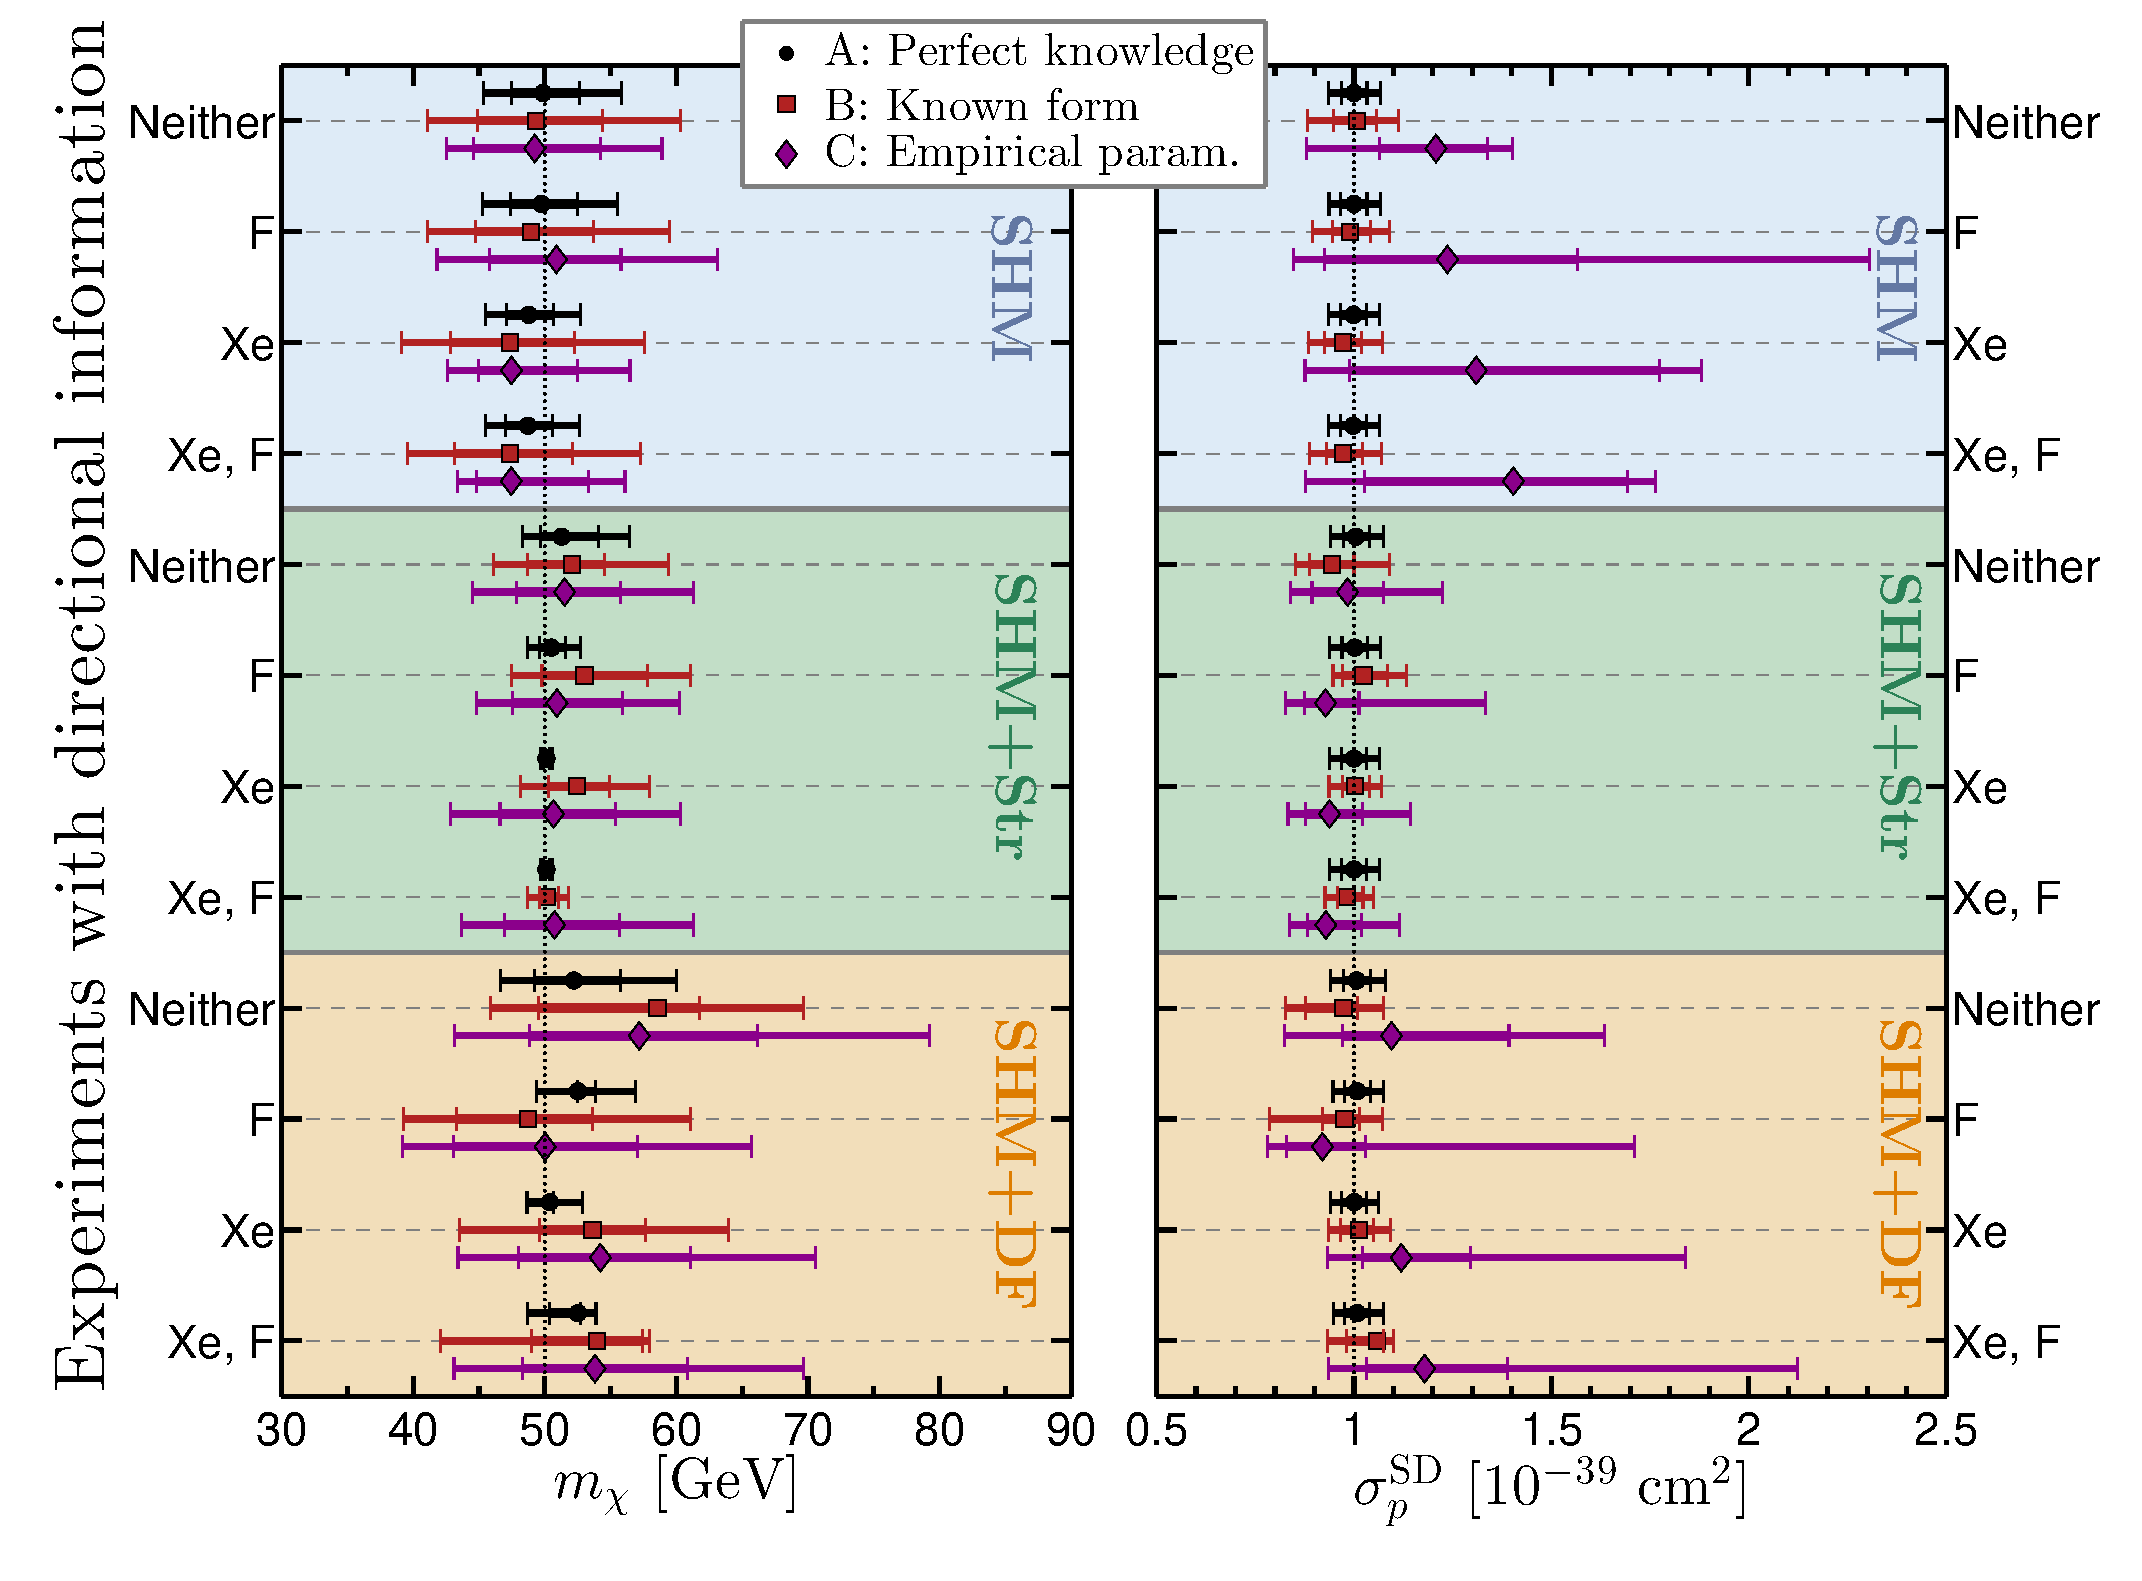
\includegraphics[width=0.95\textwidth]{Figures/mx-recon.eps}
\caption[Reconstructed confidence intervals for WIMP mass and cross section]{Reconstructed 68\% and 95\% confidence intervals for WIMP mass ({\bf left}) and SD cross section ({\bf right}) under each halo model (from top to bottom): the SHM (blue region), the SHM with stream (green) and SHM with debris flow (orange) models. The intervals are shown as a function of the amount of directional information included. The black points and error bars show the reconstruction using perfect knowledge of the DM distribution (Method A), red squares show reconstructions when the functional form is known (Method B), and purple diamonds when a general empirical form for the speed distribution is assumed (Method C). The input (i.e. correct) values are shown as vertical dotted lines.}\label{fig:mx-recon}
\end{figure}
In the right panel of Fig.~\ref{fig:mx-recon}, we show the corresponding limits on the WIMP-proton SD cross section. In this case, the contrast between Methods A \& B and Method C is more stark. Using the former two methods, reconstruction of $\sigma_p^\mathrm{SD}$ is relatively precise, with an uncertainty of less than 10\%. However, for Method C, the intervals are much wider, extending in most cases up to large values of the cross section. This results from a known degeneracy between the WIMP cross section and the shape of the speed distribution in halo-independent approaches~\cite{Kavanagh:2013wba}. An increase in the fraction of low-speed particles below the direct detection threshold has no effect on the event rate, provided the value of the cross section is increased to counteract the reduced fraction of high-speed particles.

For Method A and B we see that in most cases increasing the quantity of directional information (reading Fig.~\ref{fig:mx-recon} from top to bottom in each halo model) leads to better measurements of the WIMP mass. In contrast, the error on $\sigma_p^{\rm SD}$ found with Methods A and B is largely insensitive to the amount of directionality as the key information for reconstructing a cross section is the total number of events. For Method C, there is little increase in precision as the amount of directional information is increased; reconstruction of the WIMP mass in this case depends primarily on obtaining the correct distribution of recoil {\it energies} in each experiment. 

\subsection{Velocity distribution shape}\label{sec:directional_shape}
\begin{figure}
\centering     %%% not \center
\subfigure[{\bf SHM:} Directionality in F only.]{\label{fig:veldist-a}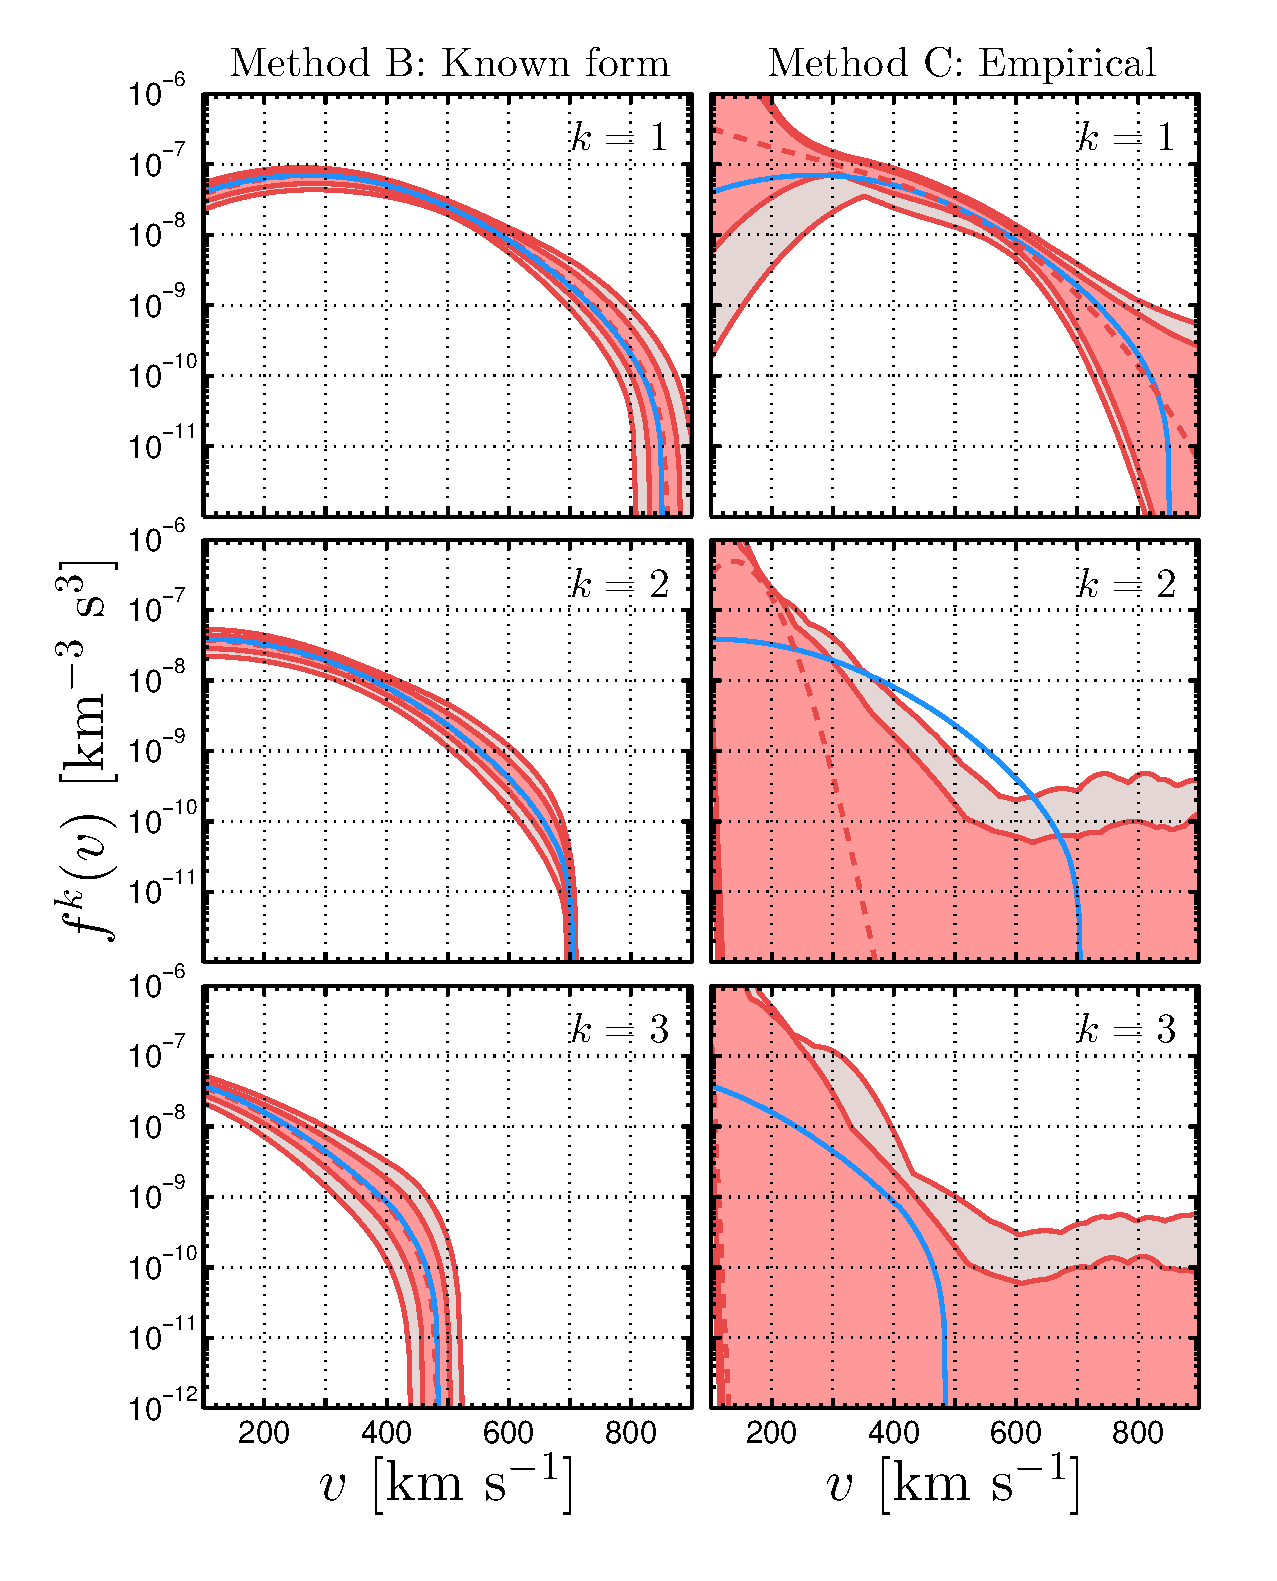
\includegraphics[width=0.49\textwidth]{Figures/veldist-SHM-Xe-N-F-D.eps}}
\subfigure[{\bf SHM:} Directionality in F and Xe.]{\label{fig:veldist-b}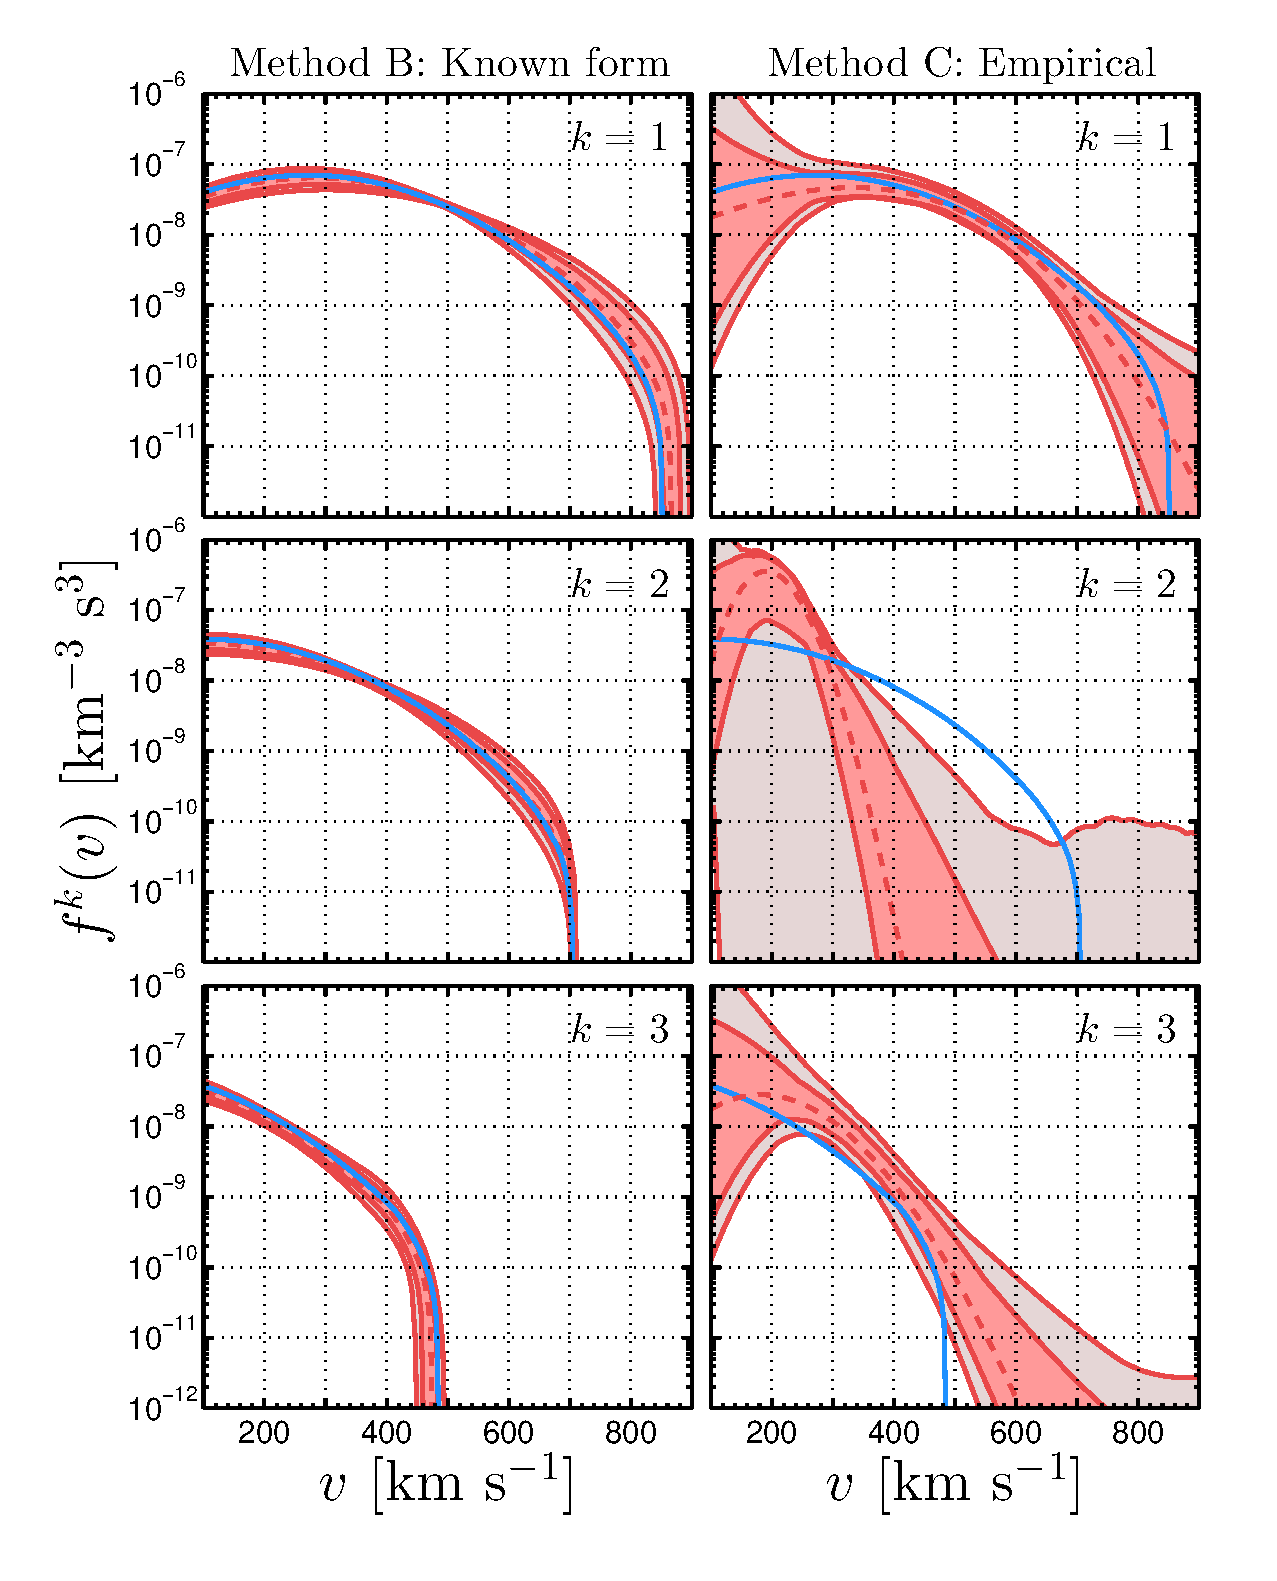
\includegraphics[width=0.49\textwidth]{Figures/veldist-SHM-Xe-D-F-D.eps}}

\subfigure[{\bf SHM+Str:} Directionality in F and Xe.]{\label{fig:veldist-c}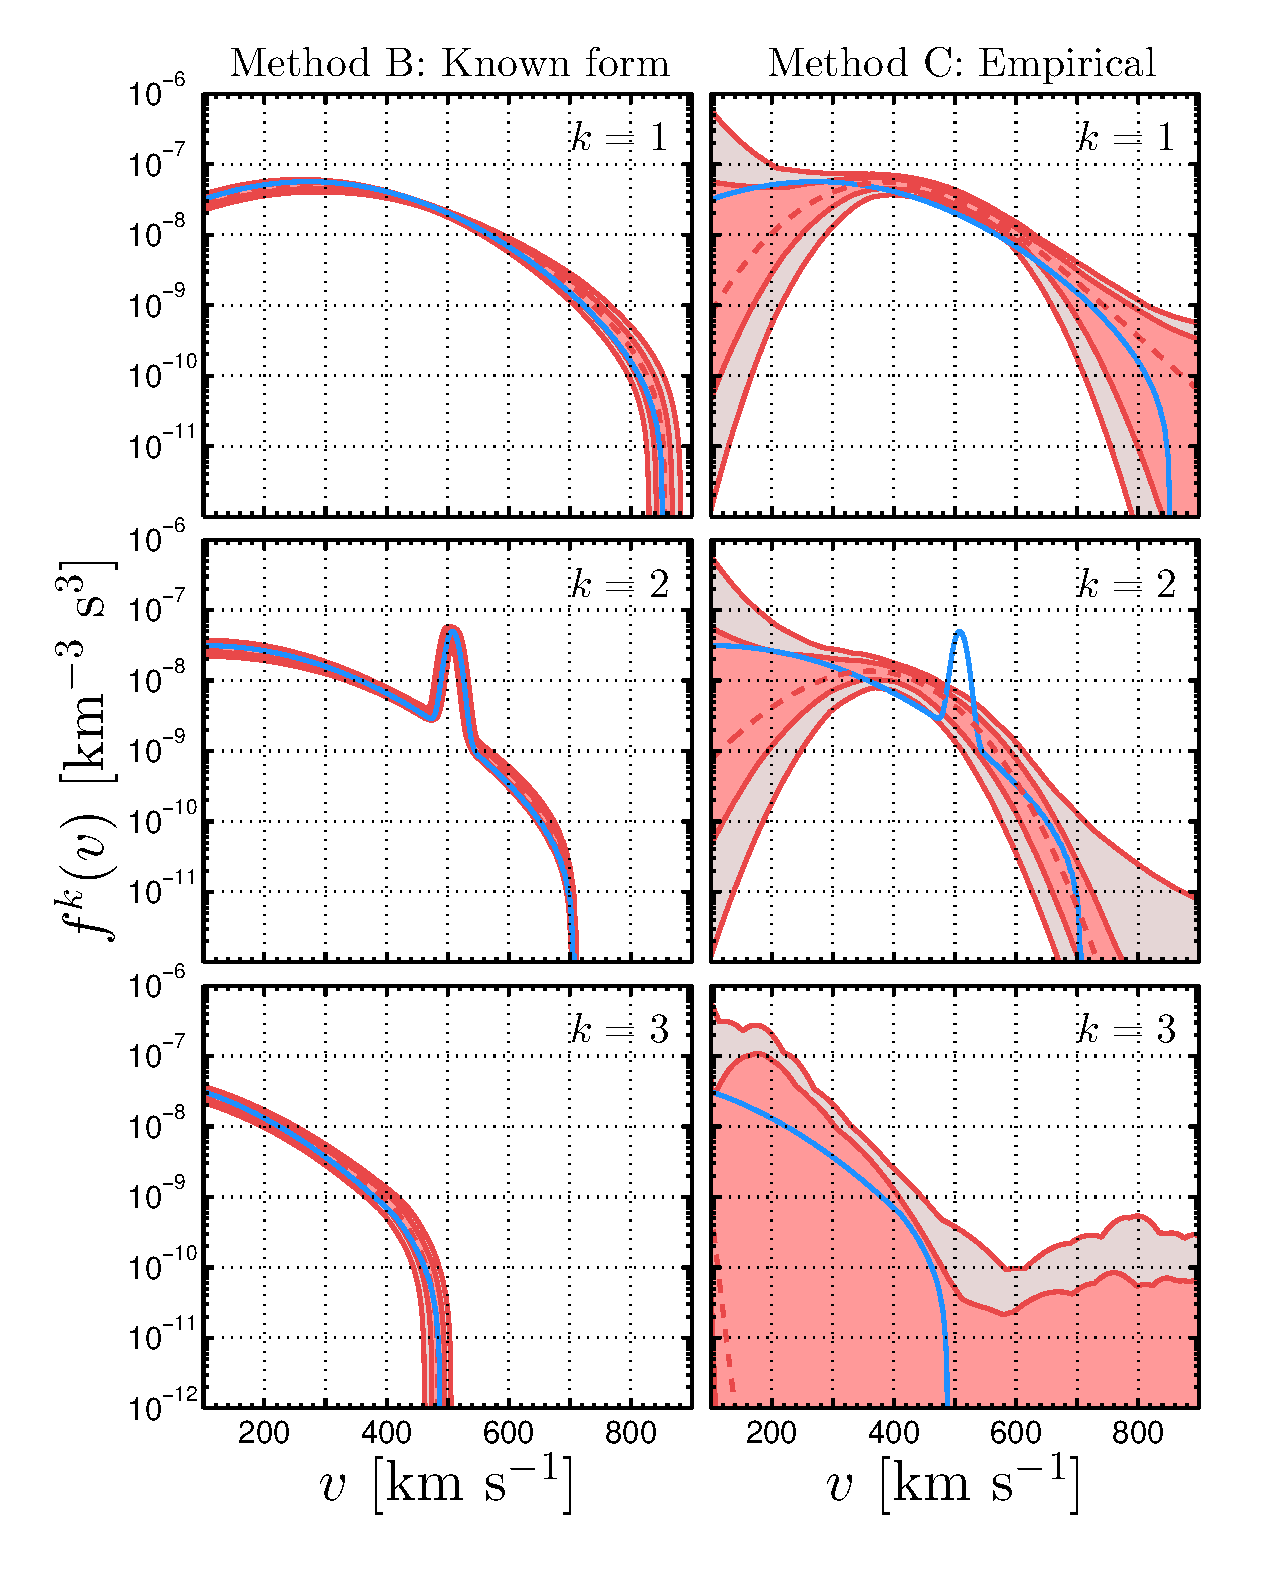
\includegraphics[width=0.49\textwidth]{Figures/veldist-STR-Xe-D-F-D.eps}}
\subfigure[{\bf SHM+DF:} Directionality in F and Xe.]{\label{fig:veldist-d}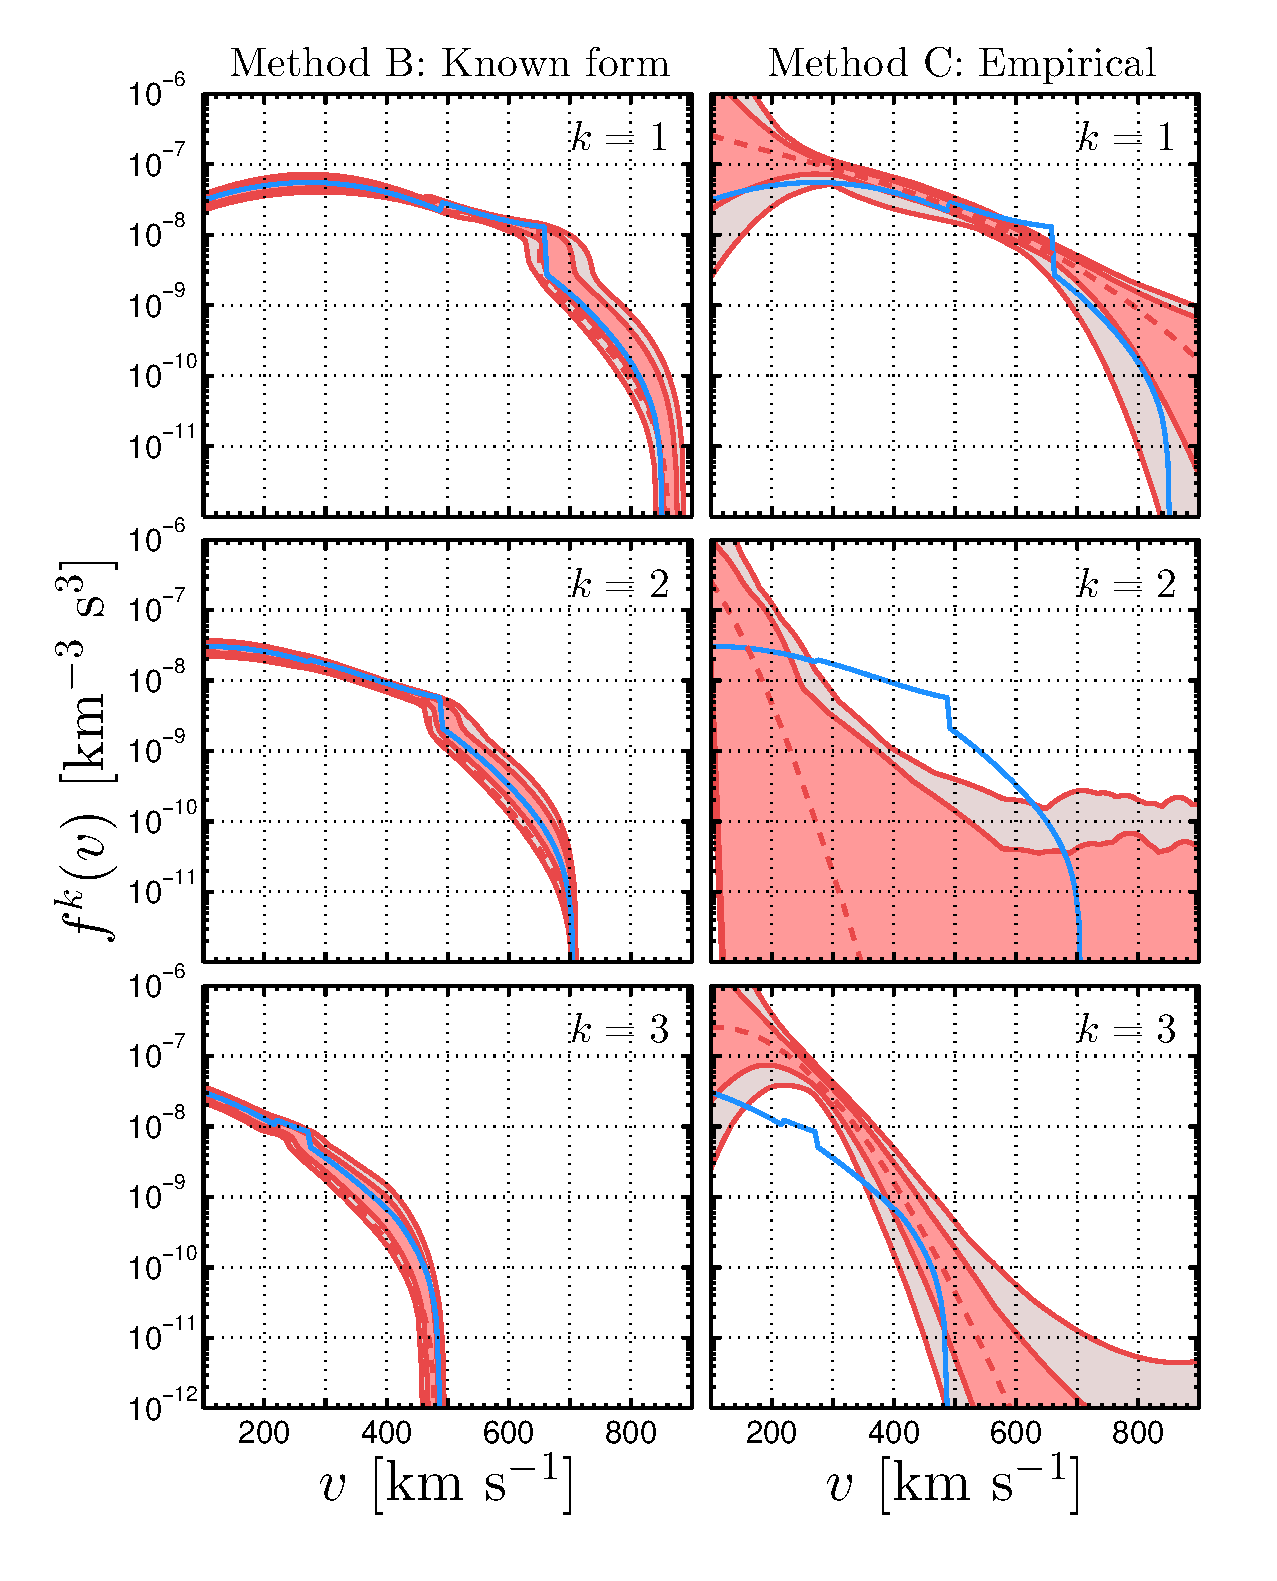
\includegraphics[width=0.49\textwidth]{Figures/veldist-DF-Xe-D-F-D.eps}}
\caption[Reconstructed binned velocity distributions]{Reconstructed velocity distribution averaged over each of the three angular bins ($k=1,2,3$) defined in Eq.~(\ref{eq:bins}). The left column in each subfigure shows the results for Method B (known functional form) while the right column shows results for Method C (empirical parameterisation). The correct underlying velocity distribution is shown with a solid blue line. The best fit reconstruction is shown as a red dashed line, while the 68\% and 95\% intervals are given by the inner and outer red shaded regions.}\label{fig:veldist}
\end{figure}

We now present results for the shape of the reconstructed velocity distribution in each of the three angular bins:
\begin{align}\label{eq:bins}
\begin{split}
{\rm `Forward\textrm{'}}\quad &k = 1: \qquad \theta \in \left[ 0, \pi/3\right]\,, \\
{\rm `Transverse\textrm{'}}\quad &k = 2: \qquad \theta \in \left[ \pi/3, 2\pi/3 \right]\,, \\
{\rm `Backward\textrm{'}}\quad &k = 3: \qquad \theta \in \left[ 2\pi/3, \pi\right]\,. \\
\end{split}
\end{align}
For the discretised velocity distribution of Method C, we simply construct the velocity distribution in the $k$th bin, $f^k(v)$, from the $\{a_m^{(k)}\}$ parameters according to Eq.~(\ref{eq:polynomialparam}). For Method B, we average the full velocity distribution (described by a given set of parameters) over each angular bin in $k$:
\begin{equation}\label{eq:fk}
f^{k}(v) = \frac{\int_{\cos(k\pi/N)}^{\cos((k-1)\pi/N)} f(\mathbf{v}) \, \mathrm{d}\cos\theta}{\cos((k-1)\pi/N) - \cos(k\pi/N)}\,.
\end{equation}
At each speed $v$, 68\% and 95\% confidence intervals are calculated from the distribution of values of $f^k(v)$ by profiling over the values at all other speeds (as well as the mass and cross section). Figure~\ref{fig:veldist} compares the reconstructed distributions $f^k(v)$ in the two Methods B and C (red curves) as well as `true' distributions obtained by applying Eq.~(\ref{eq:fk}) to the correct underlying distribution (solid blue curve). We describe each subfigure of Fig.~\ref{fig:veldist} in turn.

{\bf Figure~\ref{fig:veldist-a}} shows results for the SHM distribution with directional sensitivity in only the fluorine experiment. For Method B (left column), the best fit velocity distribution (dashed red) follows the underlying distribution closely. The strongest constraints are in the forward bin ($k=1$) in the range $v \sim 300~-~500 \kms$ where the distribution of recoils is most focused. Using Method C (right column), we also obtain a good fit to the velocity distribution in the forward bin. At high and low speeds, the confidence intervals widen as the recoil rate is insensitive to the shape of the speed distribution outside of the energy window $[E_\mathrm{th}, E_\mathrm{max}]$. In the transverse and backward bins, where very few of the fluorine events lie, the velocity distribution is also poorly constrained.

{\bf Figure~\ref{fig:veldist-b}} we now have both xenon and fluorine detectors with directional sensitivity. Comparing with the previous case, we see that the constraints are tightened. For Method B, this is perhaps most pronounced for the $k = 3$ bin due to the lower threshold of the xenon detector producing a distribution of nuclear recoils which is less strongly peaked in the forward direction. This means that more recoils are observed in the backward and transverse bins, improving the overall reconstruction. Similarly, constraints in the $k=3$ bin for Method C are also now stronger. However we note that the discretised velocity distribution in the $k=2$ bin is significantly lower than the true distribution. This is because $f(\mathbf{v})$ is in fact a strong function of angle across this bin. If we fixed $f^2(v)$ equal to the average of the true distribution across the entire bin, this would lead to an excess of recoils in the backwards direction and a deficit of recoils in the forward direction. Instead, the best fit form of $f^2(v)$ peaks at low speeds, with only a small contribution above the experimental thresholds. There is then still sufficient freedom in $f^1(v)$ and $f^3(v)$ to fit the observed distribution of recoils. 

{\bf Figure~\ref{fig:veldist-c}} shows results for the SHM+Str model when both experiments are directionally sensitive. As before, with Method B the velocity distribution is well reconstructed, and in fact achieves a slightly better reconstruction than under the SHM model due to the greater freedom in the larger parameter space. For Method C however the 4-parameter polynomial fit in each angular bin is not sufficient to pick out a feature as sharp as a stream. Nonetheless, the reconstruction does point towards an excess of particles in the $k=2$ bin in a wide range around the stream speed of $400 \kms$. To compensate, the best fit form of $f^3(v)$ is suppressed.

{\bf Figure~\ref{fig:veldist-d}} we show finally, the reconstructed SHM+DF model. For Method B, the confidence intervals are wider than before. This is because the debris flow is a much broader feature in the velocity distribution and therefore has a stronger degeneracy with the parameters of the SHM. For Method C, we see a slightly flatter reconstructed distribution in the $k=1$ bin than for previous benchmarks, as well as narrower uncertainty bands up to around $550 \kms$ caused by the enhancement in high energy recoils in the forward direction.

In this section, we have observed that a discretised parameterisation can approximate the shape of the bin-averaged velocity distribution when large numbers of events are observed in a particular direction. In other cases, there appears to be a discrepancy between the reconstructions and the underlying distribution. However, this is only a problem if we interpret the $f^k(v)$ distributions that are reconstructed as representing the average of the true speed distribution across the $k$th bin. This is a slightly unfair comparison as we should interpret the $f^k(v)$ functions as empirical fits to the full velocity distribution. As shown in the SHM+Str case, this comparison can be used to look for clear features in the distribution, but it is difficult to make statistically concrete statements about the underlying velocity distribution from the shapes of $f^k(v)$. In light of this, we now discuss some simple measures which can be used to extract information and compare different models in a more useful way.

\subsection{Velocity parameters}\label{sec:directional_parameters}
We now wish to find a model independent and simple way of discriminating between our three halo models. We can do this by mapping the reconstructions as presented in the previous section onto a set of physical parameters that can be extracted by both methods (B and C). We calculate mean values for the velocity parallel and transverse to the lab motion, $\langle v_y\rangle$ and $\langle v_T^2 \rangle$ respectively:
\begin{equation}\label{eq:vy}
\langle v_y \rangle = \int \mathrm{d}v \,\int_{0}^{2\pi} \mathrm{d}\phi \, \int_{-1}^1 \mathrm{d}\cos\theta \, (v\cos\theta)\, v^2 f(\mathbf{v}) \, ,
\end{equation}
and
\begin{equation}\label{eq:vT}
\langle v_T^2 \rangle = \int \mathrm{d}v \,\int_{0}^{2\pi} \mathrm{d}\phi \, \int_{-1}^1 \mathrm{d}\cos\theta \, (v^2(1-\cos^2\theta))\, v^2 f(\mathbf{v}) \, .
\end{equation}

\begin{figure}
\centering
	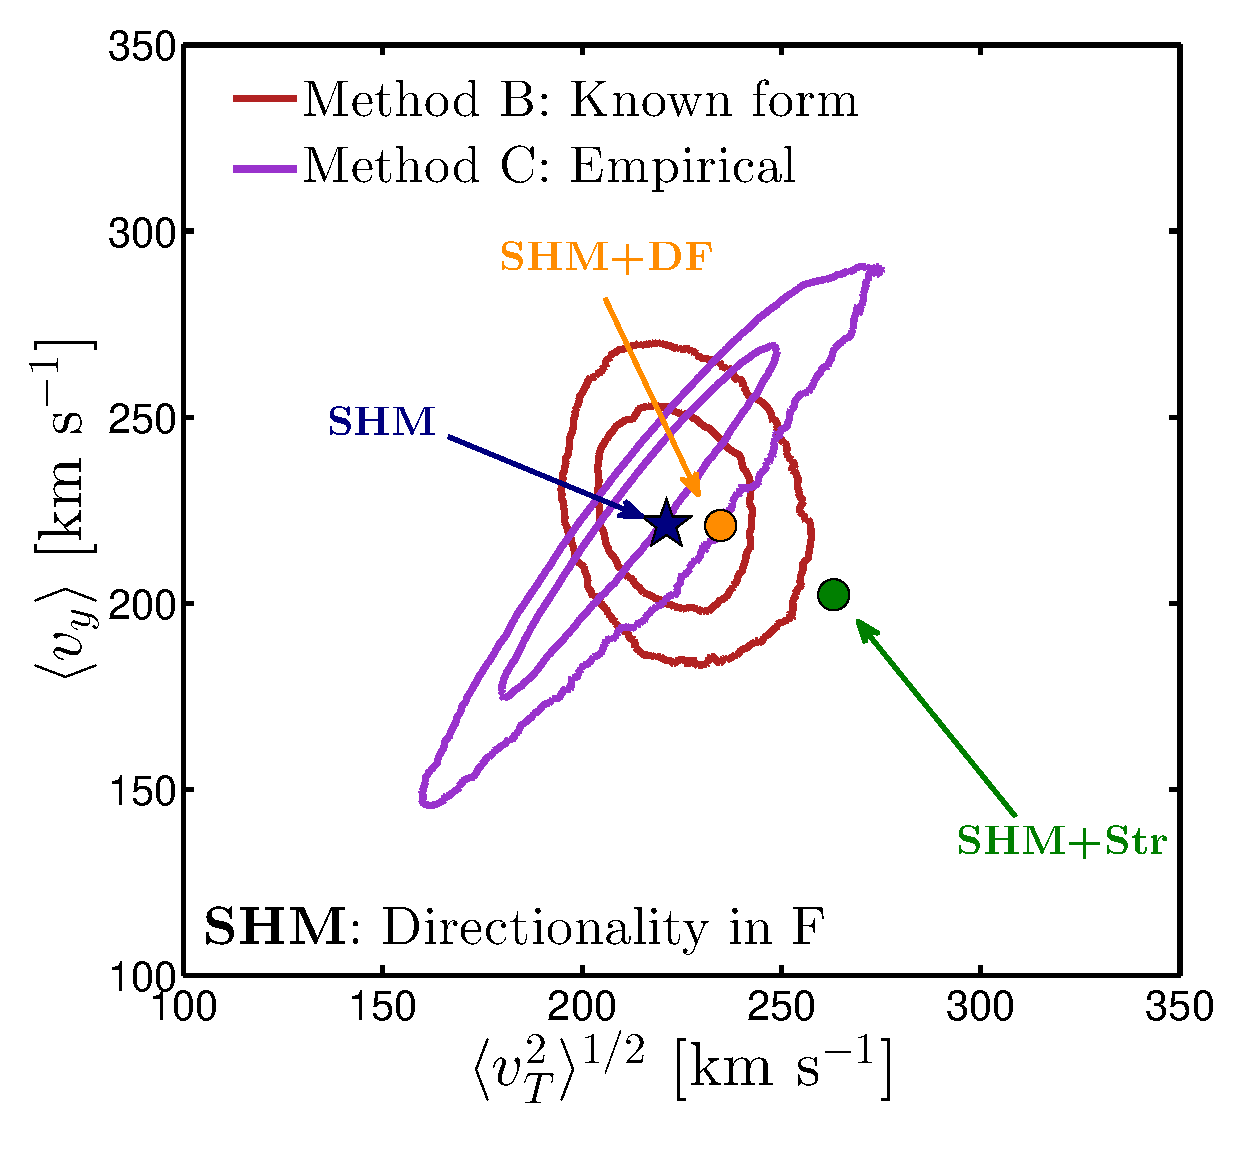
\includegraphics[width=0.32\textwidth]{Figures/vyvT-SHM-Xe-N-F-D.eps}
	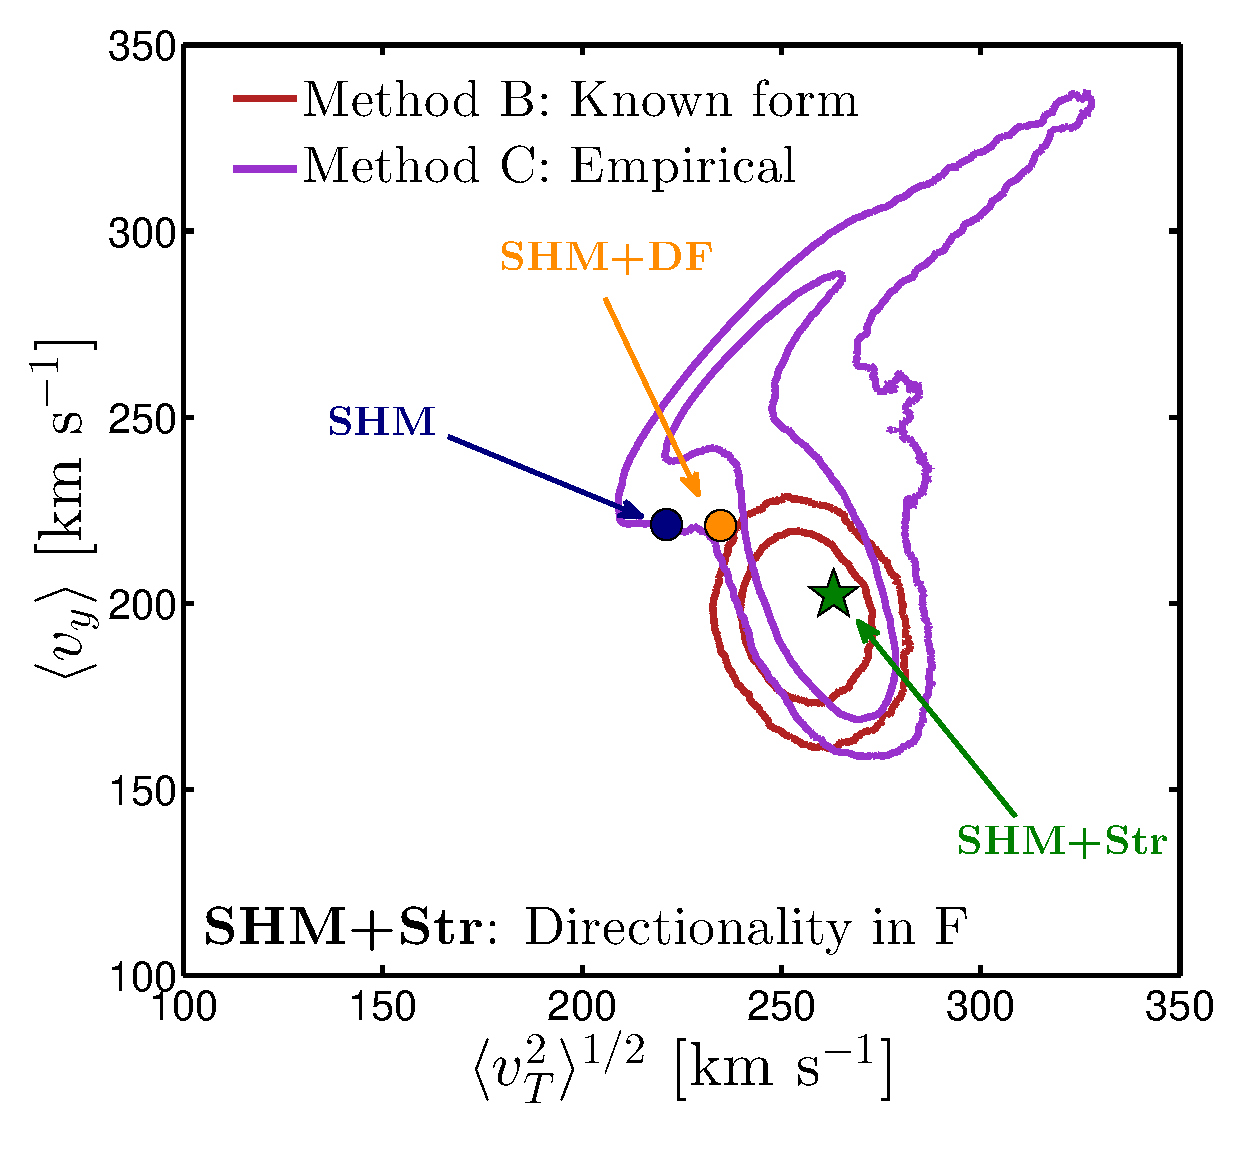
\includegraphics[width=0.32\textwidth]{Figures/vyvT-STR-Xe-N-F-D.eps}
	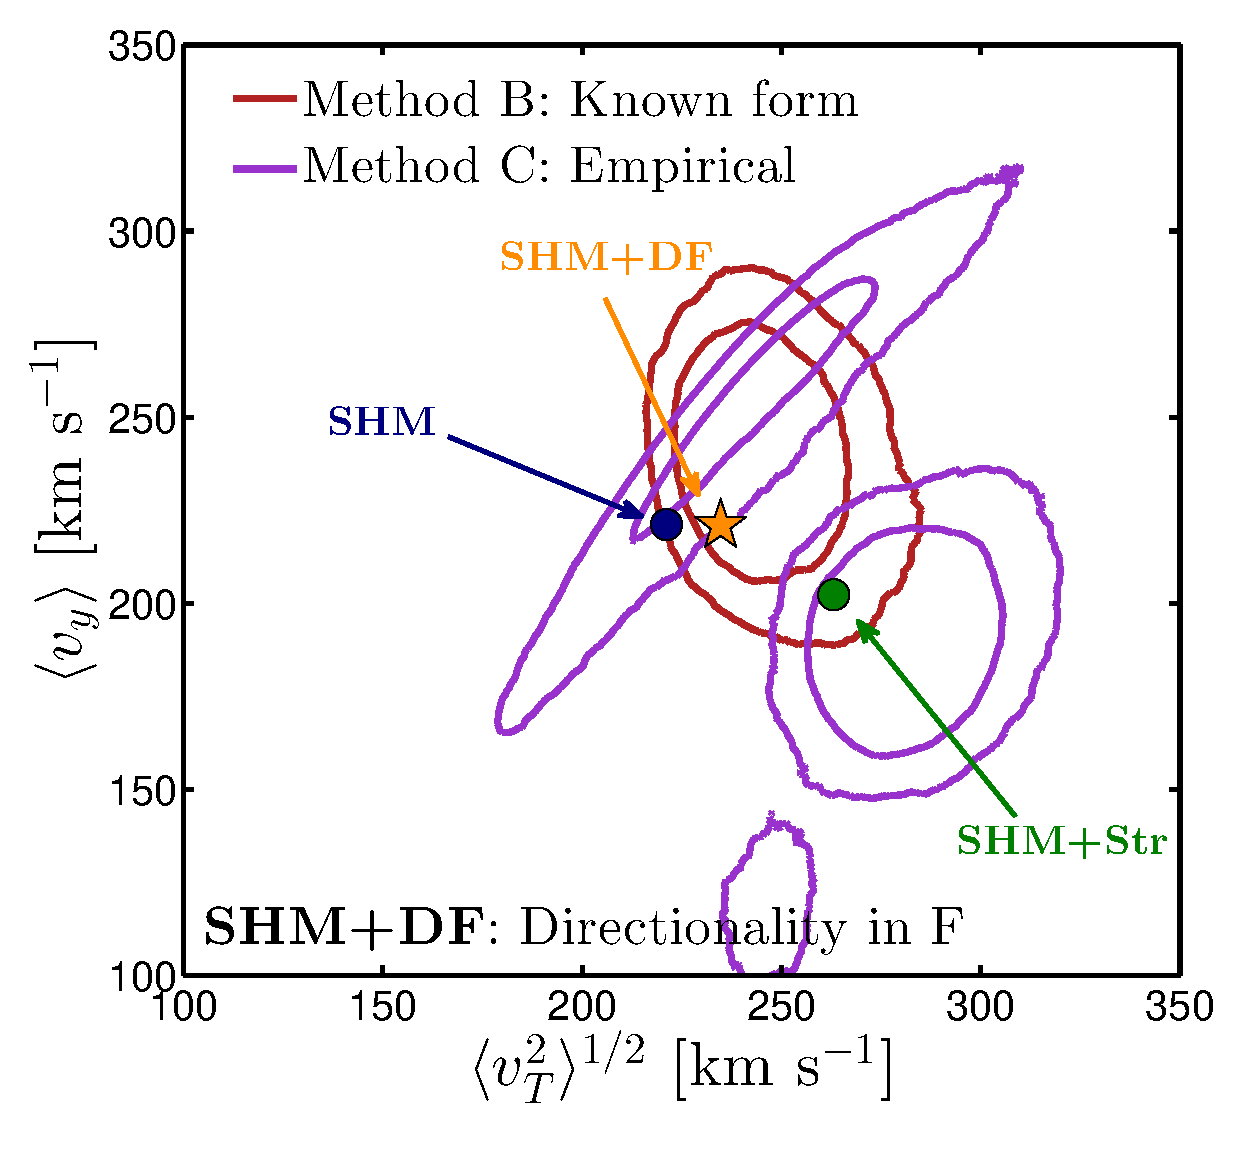
\includegraphics[width=0.32\textwidth]{Figures/vyvT-DF-Xe-N-F-D.eps}
	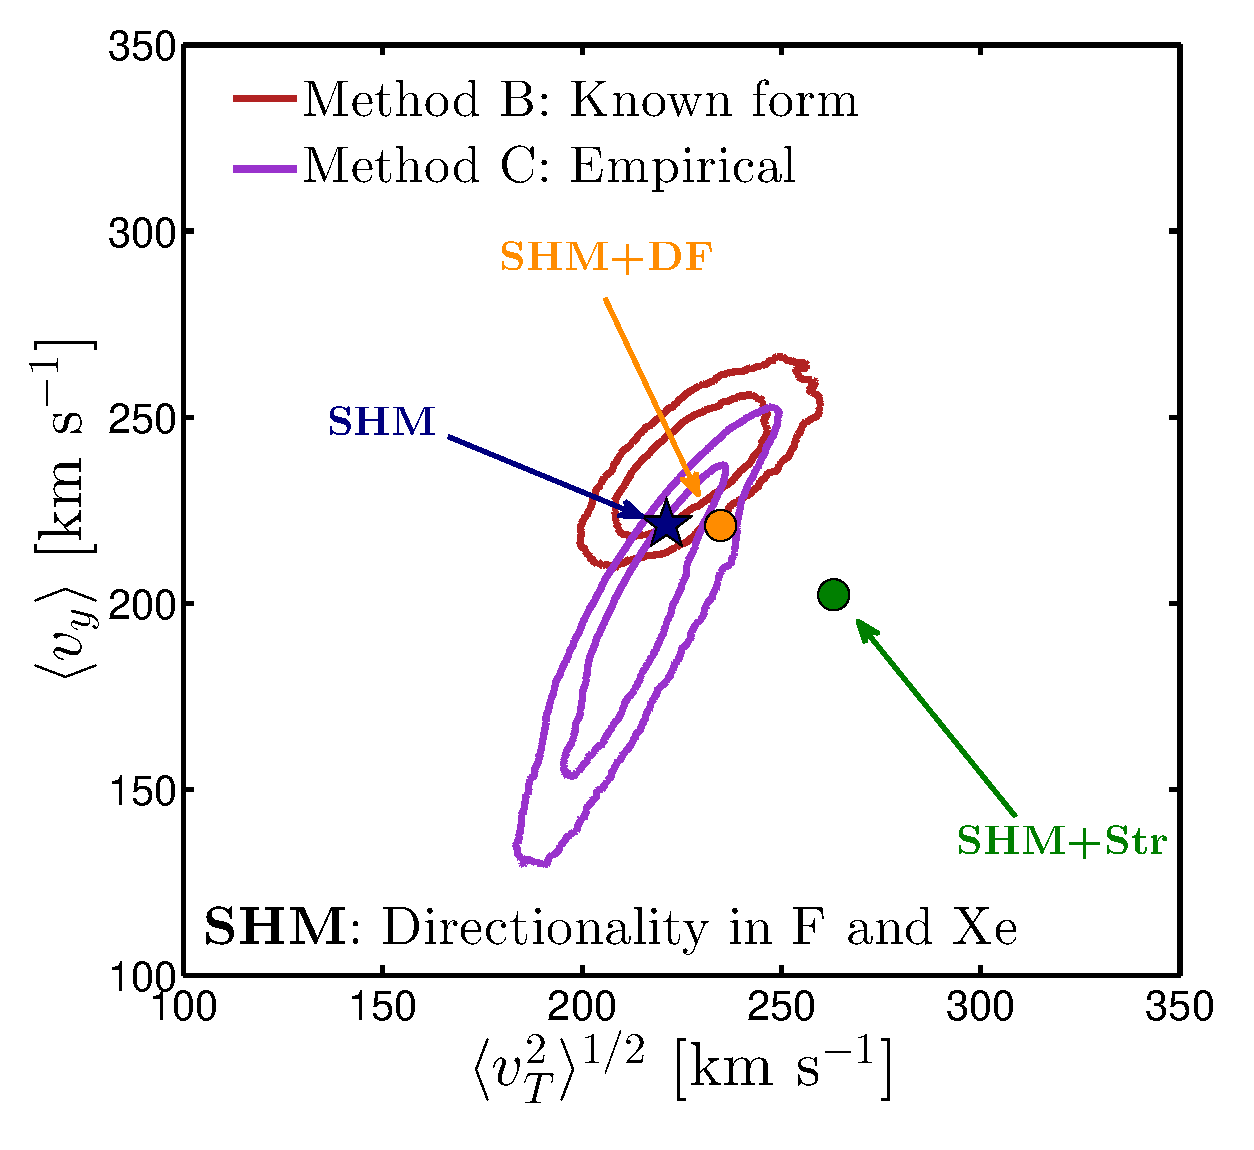
\includegraphics[width=0.32\textwidth]{Figures/vyvT-SHM-Xe-D-F-D.eps}
	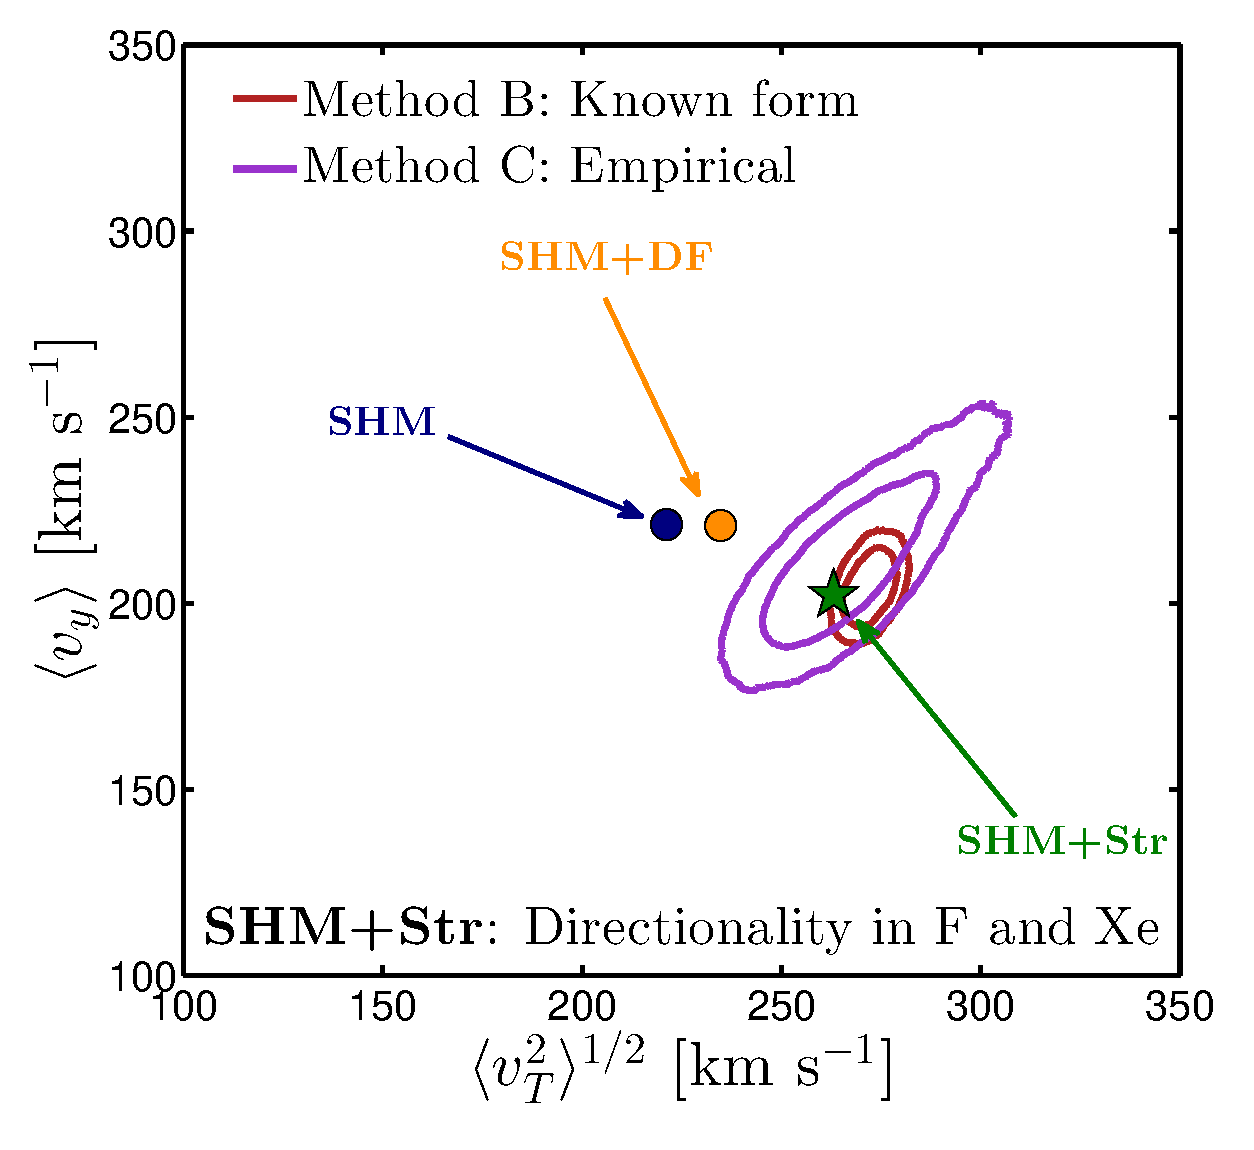
\includegraphics[width=0.32\textwidth]{Figures/vyvT-STR-Xe-D-F-D.eps}
	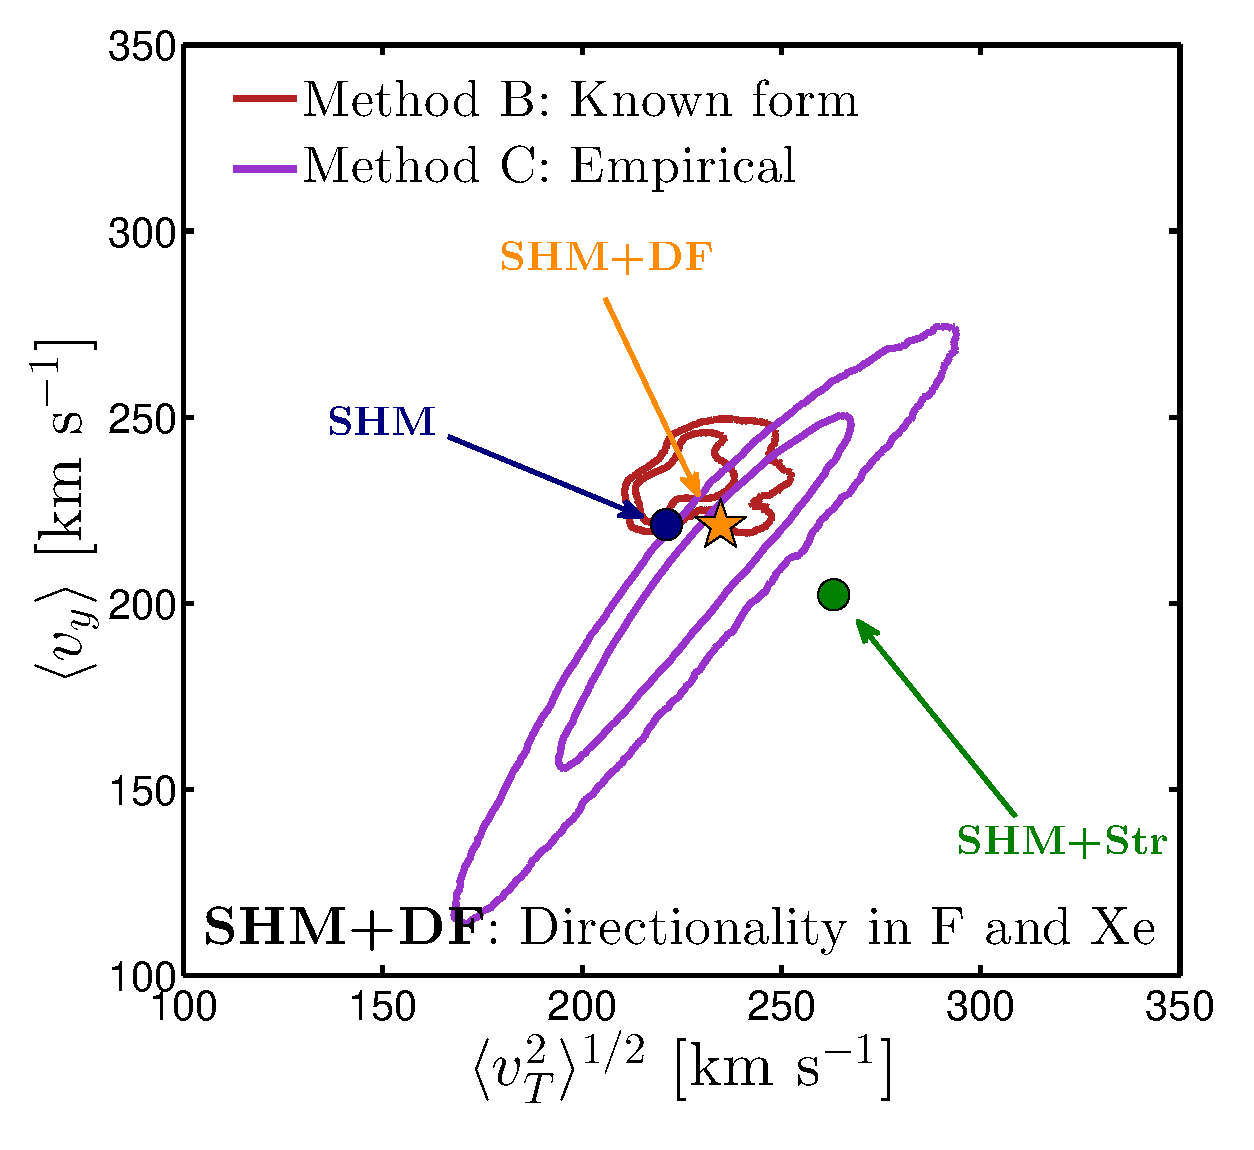
\includegraphics[width=0.32\textwidth]{Figures/vyvT-DF-Xe-D-F-D.eps}
    \caption[Reconstructed parallel and transverse velocities for each halo model]{Mean values for the DM velocity parallel and transverse to the lab velocity, $\langle v_y \rangle$, and $\langle v_T^2 \rangle^{1/2}$. The 68\% and 95\% confidence intervals obtained using reconstruction methods B and C are shown as pairs of red and purple contours respectively. We show results for all three halo models (SHM, SHM+Str and SHM+DF in each column from left to right) and for directionality in a single experiment (top row) and in both experiments (bottom). The correct values of $\langle v_y \rangle$ and $\langle v_T^2 \rangle^{1/2}$ for each halo model are shown as labelled markers (the input model is indicated with a star in each case).}\label{fig:vyvT}
\end{figure}
In Fig.~\ref{fig:vyvT} we show the reconstructed velocity distribution in each halo model mapped onto the $\langle v_y \rangle$-$\sqrt{\langle v_T^2 \rangle}$ plane. Here again we make the comparison between only fluorine having directional sensitivity (top row) and both experiments being directionally sensitive (bottom). For Method B, the values of the physical parameters ($v_0$, $\sigma_v$, $v_{\rm str}$, etc.) are typically well constrained, meaning that $\vy$ and $\vT$ are also well constrained, with roughly Gaussian error contours.  In contrast, the reconstructions using Method C exhibit a pronounced degeneracy along the direction of $\vy \propto \vT$ for many of the benchmarks. This is due to the fact that the $k=1$ and $k=3$ bins contribute to the mean values of both the forward \textit{and} transverse DM speeds. For example, increasing $f^1(v)$ leads to an increase in $\vy$ but also a proportional increase in $\vT$, because the particles are assumed to be distributed equally in $\theta$ across the bin. The position of the contours in $\vT$ is typically dominated by the $k=2$ bin, which contributes to $\vT$ and not to $\vy$. 

For both reconstruction methods and for directionality in either one or both experiments, the underlying benchmark values of $\vy$ and $\vT$ always lie within the 95\% confidence regions. The SHM and SHM+DF models are hardest to distinguish. The debris flow is isotropic in the Galactic frame, so the net velocity of the DM particles in the lab frame is due entirely to $\textbf{v}_\textrm{lab}$. Thus, we have $\vy \sim v_0$ as in the SHM. The debris flow is a rather broad feature leading only to a mild increase in $\vT$. Indeed, with the SHM benchmark dataset, the SHM+DF model cannot be rejected at the 95\% confidence level using either reconstruction method.  

The SHM+Str is much more easily distinguished from the other two benchmarks. The stream velocity is almost perpendicular to the Earth's velocity, leading to a decrease in $\vy$ and a marked increase in $\vT$. For the SHM mock dataset (left column), the SHM+Str is clearly excluded with both Methods, even when only the fluorine detector has directionality. Under the SHM+Str dataset the addition of the stream leads to a mild increase in the number of fluorine events in the transverse recoil direction, while still producing no events in the backward direction. This data can be well fit by adding a substantial population of particles in the $k=2$ bin (causing the lower round part of the contours in the upper middle panel of Fig.~\ref{fig:vyvT}) or alternatively by enhancing the forward $k=1$ population at low speeds (causing the upper straight part of the contours). Including xenon directionality (lower middle panel of Fig.~\ref{fig:vyvT}), adds roughly equal numbers of forward and transverse recoils, breaking the degeneracy and allowing the SHM+Str model to be unequivocally distinguished from the other benchmarks.

Using the SHM+DF dataset  with directionality in fluorine only (upper right panel of Fig.~\ref{fig:vyvT}), we notice there are three distinct regions fit by Method C. The three regions correspond to enhanced populations of DM particles in each bin. The Debris Flow contributes in all 3 angular bins and will typically produce higher energy recoils than the SHM alone (as $v_f > v_0$). An increased high-speed population in any of the velocity bins will then improve the fit to the data. Once again, adding xenon directions breaks the degeneracy between the three regions and in this case the SHM+Str benchmark can be rejected.

These results indicate that mapping the reconstructed velocity distributions onto the parameters $\vy$ and $\vT$ can be a reliable and unbiased way of trying to distinguish different underlying halo models. The SHM and SHM+DF models are typically difficult to distinguish, while the SHM+Str has sufficiently different properties (a large transverse velocity) that it can be clearly excluded in many cases.

\subsection{Folded reconstructions}
As discussed in Sec.~\ref{sec:directional_expts}, a major concern for current directional detection experiments is the ability to measure the forward or backward going sense of a reconstructed recoil track. We define the `folded' recoil spectrum that would be observed in experiments without any head-tail effect as,
\begin{equation}
 \frac{\mathrm{d}^2R_\mathrm{fold}}{\mathrm{d}E_r\mathrm{d}\Omega_r} = \frac{\mathrm{d}^2R}{\mathrm{d}E_r\mathrm{d}\Omega_r}\bigg|_{-\qhat}+\frac{\mathrm{d}^2R}{\mathrm{d}E_r\mathrm{d}\Omega_r}\bigg|_{+\qhat} \, .
\end{equation}
Following the results of Sec.~\ref{sec:directional_parameters} we show again the expectation values for the parallel and transverse velocities with respect to the direction of the Earth's motion. In this case for brevity we include only the result for the case in which both fluorine and xenon experiments have directional sensitivity, only now we remove their ability to tell the forward or backward going sense of their nuclear recoils. The results are shown for each halo model in Fig.~\ref{fig:vyvT-folded}.

\label{sec:folded}
\begin{figure*}[t]
	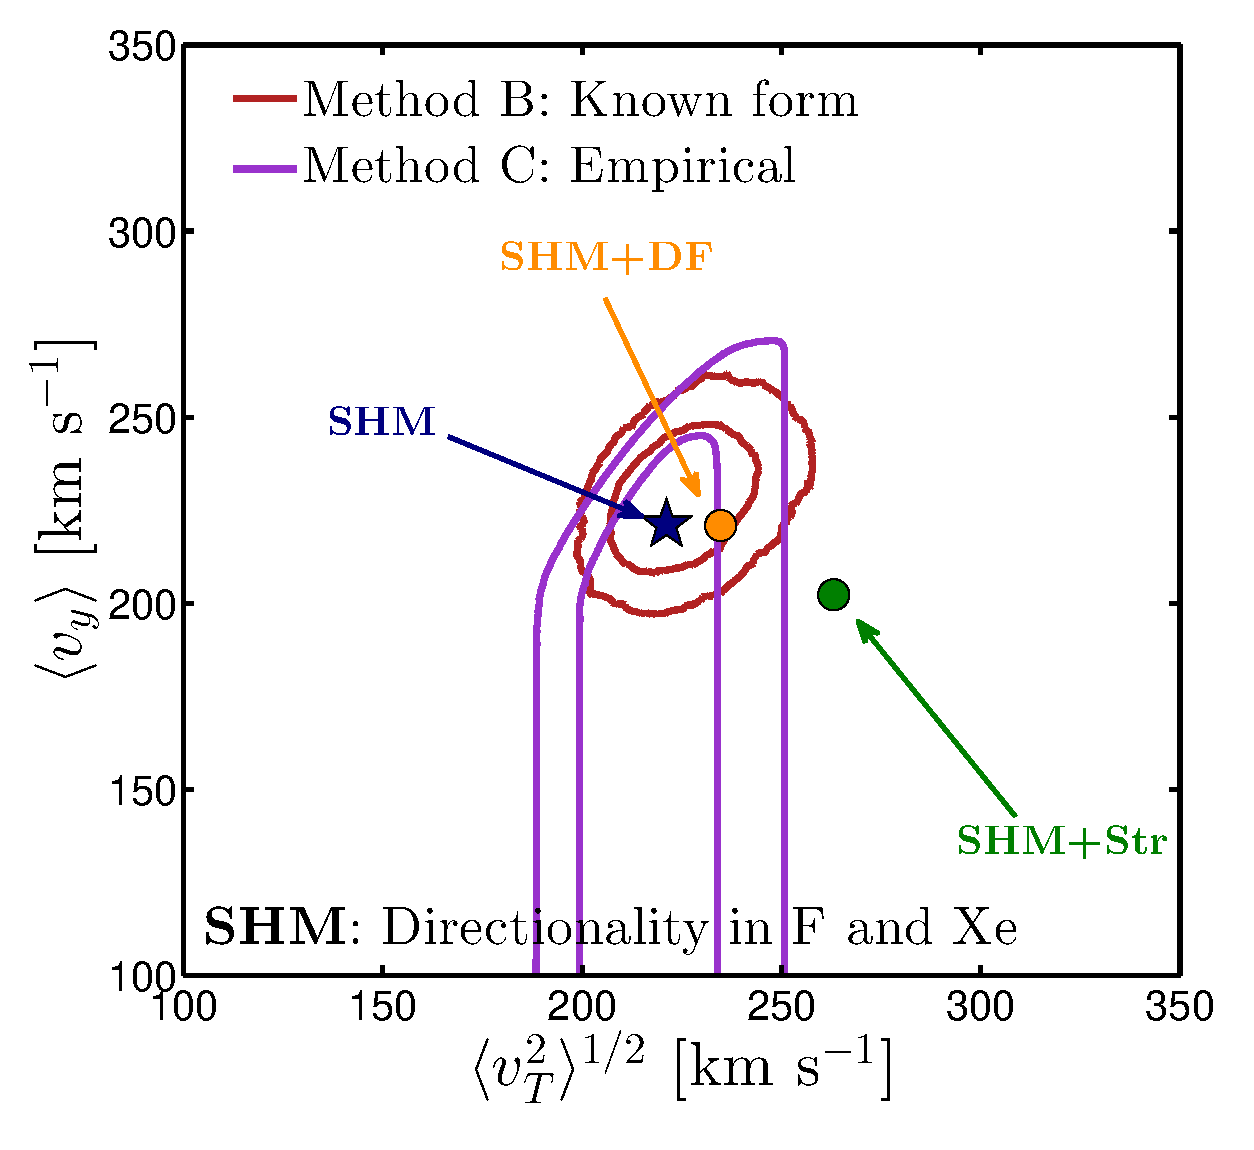
\includegraphics[width=0.32\textwidth]{Figures/vyvT-SHM-Xe-D-F-D-folded.eps}
	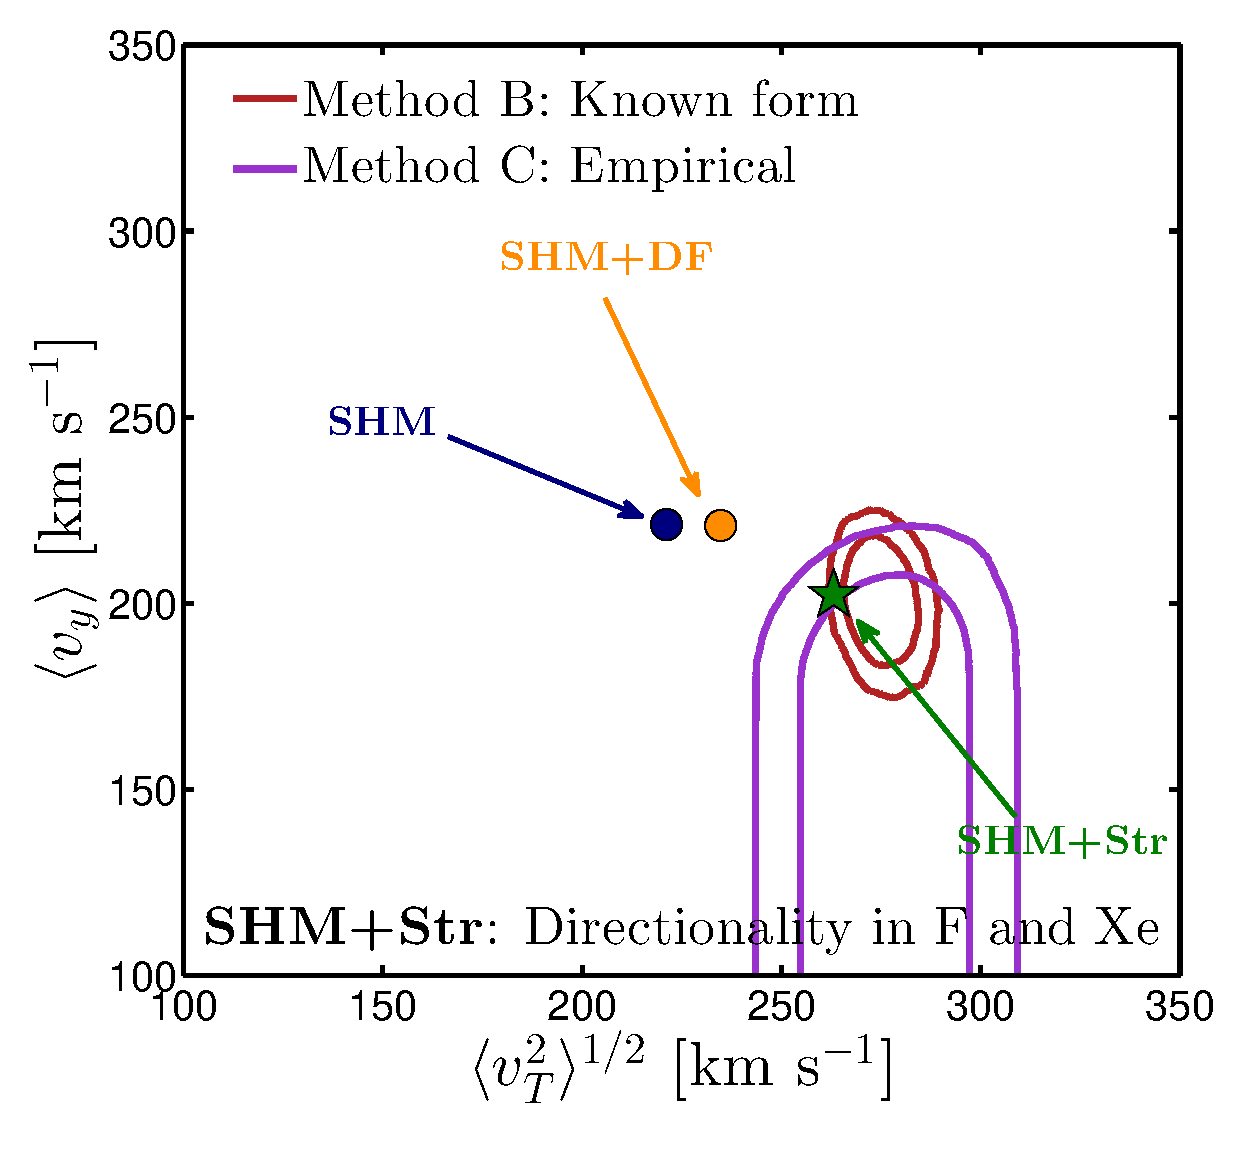
\includegraphics[width=0.32\textwidth]{Figures/vyvT-STR-Xe-D-F-D-folded.eps}
	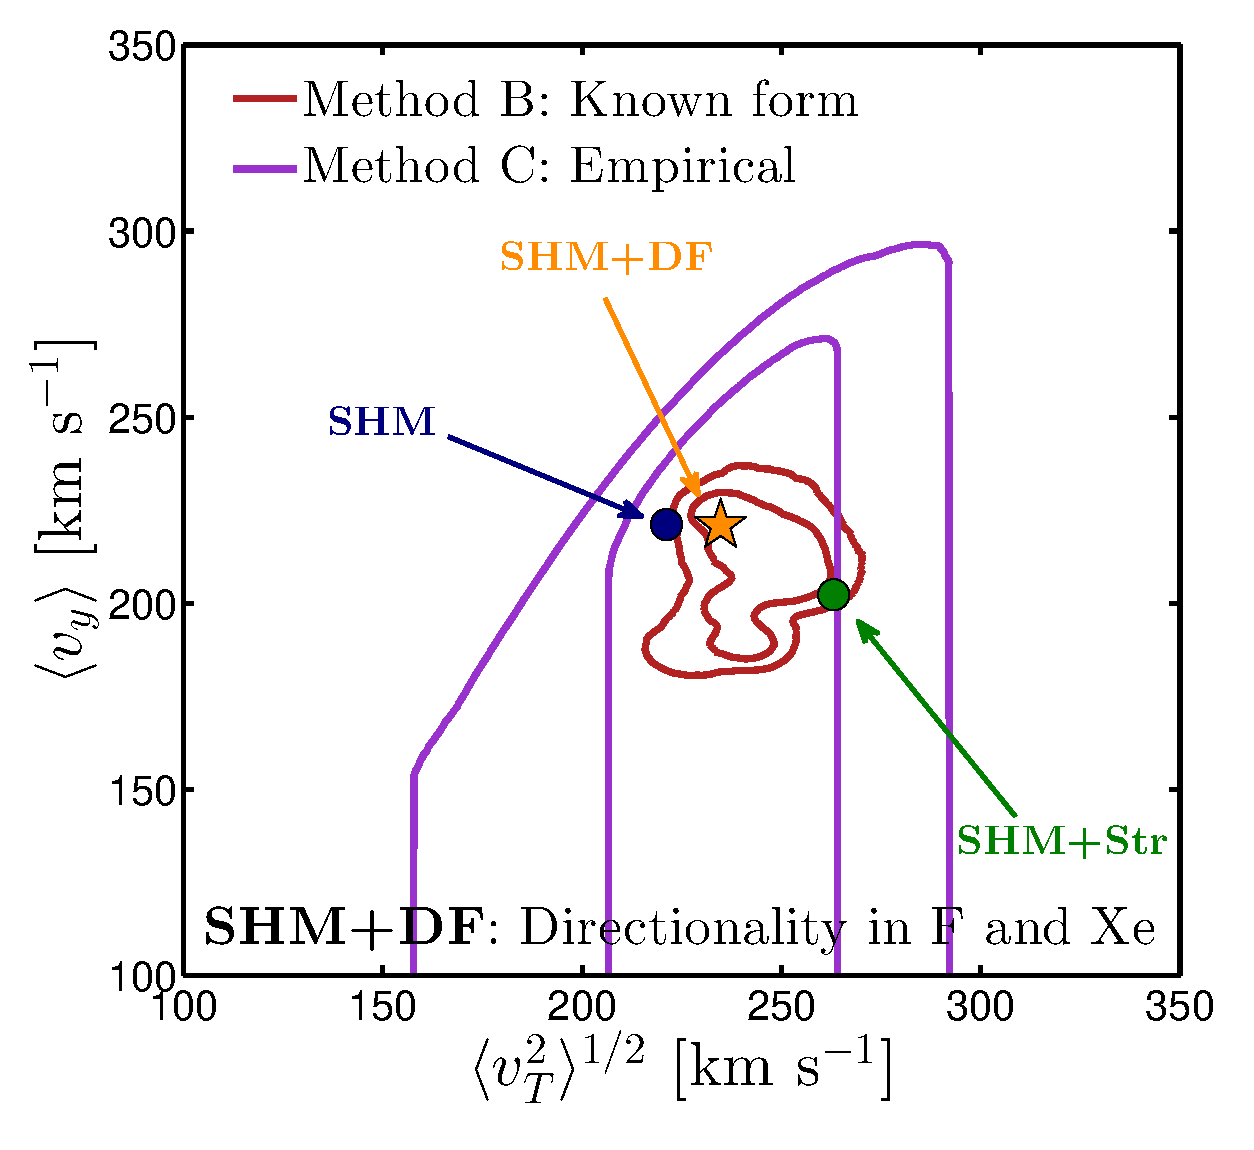
\includegraphics[width=0.32\textwidth]{Figures/vyvT-DF-Xe-D-F-D-folded.eps}
    \caption[Reconstructed parallel and transverse velocities with folded data]{Mean values for the DM velocity parallel and transverse to the lab velocity, $\langle v_y \rangle$, and $\langle v_T^2 \rangle^{1/2}$, reconstructed when both experiments have directional sensitivity but lack sense recognition. The 68\% and 95\% confidence intervals obtained using reconstruction methods B and C are shown as pairs of red and purple contours respectively. We show the results for each halo model (from left to right), the SHM, the SHM+Str and SHM+Debris flow models. For Method C (purple), the contours extend all the way down to negative values of $\vy$, but for clarity we show only the region of parameter space near the benchmark values.}\label{fig:vyvT-folded}
\end{figure*}
With the removal of sense recognition the pronounced dipole feature of the angular distribution of recoils is reduced. Hence our directional experiments can no longer extract information about the asymmetry between forward and backward going recoils. For Method B there is only a small increase in the size of the contours for the SHM and SHM+Str models as in these cases there are large populations of recoils transverse to the folding so there is not a large reduction in sensitivity to the parameters that are being reconstructed. Whilst there is a larger uncertainty in the full 3-dimensional stream velocity in Method B, this uncertainty is disguised by the mapping onto $\vy$ and $\vT$ and the SHM and SHM+Str benchmarks can still be distinguished. However in the case of the SHM+DF model there is a moderate increase in the size of the contours in $\vy-\vT$. This is because some of the information regarding the velocity of the debris flow is encoded in the forward-backward asymmetry of the recoils.

For Method C, however, we see a complete degeneracy appearing in the results for all three halo models between positive and negative values of $v_y$ (although for clarity we display only positive values of $v_y$ here). This is to be expected as the folded distribution measured by Method C has no distinction between $\vy$ running parallel or anti-parallel to the Earth's motion. However as we have not removed as much transverse information, the shape of the contours in the $\vT$ direction remain relatively unchanged for the SHM and SHM+Str models. In particular, for data under the SHM+Str benchmark, the SHM and SHM+DF benchmarks can still be rejected at the 95\% confidence level. However, this is not the case for the SHM+DF model; the debris flow component has populations in both transverse and parallel directions so there is a major increase in the size of the contours in both $\vy$ and $\vT$. In this case all three benchmarks lie within the 68\% region.

\subsection{Summary}
In this Chapter we have explored a number of methods for reconstructing the velocity distribution from future directional experiments. We have focused in particular on using a general, empirical parameterisation to fit the velocity distribution and compared this with the case where the underlying form of the velocity distribution is known. This allows us to understand whether the two methods lead to different reconstructed parameter values (which may be indicative of biased reconstructions) and how much the constraining power of the experiments changes as we open up the parameter space with a more general fit.

Previous works have demonstrated that the WIMP mass can be recovered from non-directional direct detection experiments without making assumptions about the form of the speed distribution \cite{Peter:2011eu,Kavanagh:2013wba}. As we show in Fig.~\ref{fig:mx-recon}, such astrophysics-independent approaches can be successfully extended to directional experiments. In particular, the use of an approximate, discretised velocity distribution does not spoil the accurate reconstruction of the WIMP mass. Our empirical parameterisation typically leads to larger uncertainties than when the underlying form of the distribution is known, but we see no evidence of bias.

For reconstructing the velocity distribution, as demonstrated in Sec.~\ref{sec:directional_shape}, looking at the binned form may allow us to pick out key features but it is generally difficult to make comparisons or draw meaningful conclusions. Instead, we construct confidence intervals for the velocity averages $\vy$ and $\vT$. These measures of the shape of the distribution allow us to distinguish robustly between different underlying halo models. We find that with directionality only in a fluorine experiment, it may be possible to detect or reject the presence of a substantial stream with 95\% confidence. This is an improvement upon the results of Sec.~\ref{sec:directional_streams} as in this case we have assumed no knowledge about the underlying distribution and relies on fewer directional events. However, more isotropic features such as a debris flow are more difficult to distinguish from the SHM. Adding directionality in a xenon experiment allows us to break degeneracies in the shape of the velocity distribution and leads to good discrimination between models with and without a stream. The SHM and SHM+DF models remain harder to distinguish using this method, whether the underlying functional form is known or not.

In experiments without the ability to determine the sense of the nuclear recoils we see that the discretised approach suffers. This is because the $N=3$ binning is effectively reduced to 2 as the forward and backward bins are folded. The result of this is that it becomes impossible to precisely measure the average speed in the direction of the folding due to a degeneracy between positive and negative values. This is in line with the results of previous studies~\cite{Green:2007at,Billard:2014ewa} finding that the lack of sense recognition greatly reduces the power of directional experiments.

The benchmark examples we have chosen in this work enable us to broadly compare the success of a discretised parameterisation of the velocity distribution under a range of scenarios. However the parameter space that describes different classes of substructure, for instance streams, is large. It is unlikely that the conclusions drawn from our benchmark (which includes a rather large stream component) can be extended generally over the range of possible stream speeds and directions. However, we have demonstrated that an empirical parameterisation can accommodate a wide range of underlying velocity distributions without a large loss in sensitivity compared to when the functional form is fixed and known.

In this Chapter we have considered only ideal direct detection experiments. Experimental complications such as finite energy and angular resolution, as well as the possibility of lower-dimensional readouts, will of course affect the reconstruction of the DM parameters in real experiments. We note, however, that the angular binning procedure we have used in the empirical reconstructions may be a natural way to account for finite angular resolution. If the angular resolution (typically in the range 20$\,^{\circ}$~-~80$\,^{\circ}$ \cite{Billard:2012bk}) is smaller than the binning angle (here, $60^\circ$), the inclusion of these effects should have little impact on the results.

\section{Final remarks}\label{sec:directional_finalremarks}
In spite of the open questions that still remain, the studies we have presented here show that for exploring the full three-dimensional local velocity distribution, which is a primary motivation for directional experiments, one can make significant progress without assumptions about the underlying astrophysics. The methods we have presented allow one to combine directional and non-directional experiments in a general way in order to accurately reconstruct the WIMP mass, identify broad features in the DM velocity distribution and perhaps even distinguish different underlying models for the DM halo. If with some future data, the use of model independent or non-parametric methods points towards the existence of a velocity distribution that departs from a simple isotropic assumption, then this would allow an unbiased transition to model dependent fits to particular types of substructure, for instance the case study of tidal streams we explored in Sec.~\ref{sec:directional_streams}. In any case we conclude by remarking that directional detectors represent an exciting prospect for uncovering the structure of the local dark matter halo. In the future this may lead the way to development of WIMP `astronomy' and the archaeology of the Milky Way.